\documentclass[10pt,a4paper]{article}
\usepackage[utf8]{inputenc}
\usepackage[T1]{fontenc}
\usepackage[spanish,es-tabla,es-nodecimaldot,es-lcroman]{babel}

% =========================================================================
% TIPOGRAFÍA Y MICROTIPOGRAFÍA
% =========================================================================
\usepackage{lmodern}
\AtBeginDocument{\DeclareFontShape{T1}{lmr}{bx}{sc}{<->ssub*lmr/bx/n}{}}
\usepackage{microtype}
\usepackage{amsmath,mathtools}
\usepackage[top=2.1cm, bottom=2.1cm, left=2.1cm, right=2.1cm]{geometry}
\usepackage{xcolor}
\usepackage{graphicx,booktabs,longtable,array,tabularx,makecell}
\usepackage{enumitem}
\usepackage{float,placeins,setspace}
\usepackage[font=small,labelfont={bf},skip=6pt]{caption}
\usepackage{titlesec}
\usepackage[titles]{tocloft}
\usepackage{tcolorbox}
\tcbuselibrary{skins,breakable}
\usepackage{listings}
\usepackage{fancyhdr}
\usepackage[hidelinks]{hyperref}

% =========================================================================
% ESTILO EDITORIAL MONOCROMÁTICO SOBRIO (NEGRO, BLANCO Y GRISES NEUTROS)
% =========================================================================
\setstretch{1.15}
\setlength{\emergencystretch}{2em}
\setlength{\parskip}{5pt}
\setlength{\headheight}{23pt}
\renewcommand{\arraystretch}{1.3}
\setlength{\tabcolsep}{7pt}
\graphicspath{{img/}}

\hypersetup{
  hidelinks,
  colorlinks=false,
  pdfauthor={Grupo 9 - UNSAAC},
  pdftitle={Evaluación Comparativa de Tres Arquitecturas CNN para Clasificación de Lesiones Cutáneas Pigmentadas mediante Dermatoscopia (HAM10000)}
}

% =========================================================================
% ENCABEZADO Y PIE DE PÁGINA
% =========================================================================
\pagestyle{fancy}
\fancyhf{}
\fancyhead[L]{\small\textbf{UNSAAC} \textcolor{black!75}{-- Visión por Computador (2026-II)}}
\fancyhead[R]{\small\textcolor{black!75}{Grupo N.\ 9 $\cdot$ Clasificación Dermatoscópica (HAM10000)}}
\fancyfoot[L]{\footnotesize\textcolor{black!75}{Informe Técnico Científico}}
\fancyfoot[R]{\small\textbf{\thepage}}
\renewcommand{\headrulewidth}{0.5pt}
\renewcommand{\footrulewidth}{0.4pt}
\renewcommand{\headrule}{\hbox to\headwidth{\color{black}\leaders\hrule height \headrulewidth\hfill}}
\renewcommand{\footrule}{\hbox to\headwidth{\color{black!25}\leaders\hrule height \footrulewidth\hfill}}

% =========================================================================
% JERARQUÍA DE TÍTULOS
% =========================================================================
\titleformat{\section}
  {\Large\bfseries\color{black}}
  {\thesection.}{0.55em}{}[\vspace{3pt}{\color{black}\titlerule[0.8pt]}]
\titleformat{\subsection}
  {\large\bfseries\color{black}}
  {\thesubsection}{0.55em}{}
\titleformat{\subsubsection}
  {\normalsize\bfseries\color{black!75}}
  {\thesubsubsection}{0.55em}{}
\titlespacing*{\section}{0pt}{16pt}{7pt}
\titlespacing*{\subsection}{0pt}{11pt}{4pt}
\titlespacing*{\subsubsection}{0pt}{8pt}{3pt}

% =========================================================================
% ÍNDICES COMPACTOS Y LEGIBLES (CORRIGE SOLAPE EN SECCIONES >= 10)
% =========================================================================
\setlength{\cftbeforesecskip}{2.2pt}
\setlength{\cftbeforesubsecskip}{0pt}
\setlength{\cftsecnumwidth}{2.2em}
\setlength{\cftsubsecindent}{2.0em}
\setlength{\cftsubsecnumwidth}{2.8em}
\renewcommand{\cftsecfont}{\bfseries\small\color{black}}
\renewcommand{\cftsecpagefont}{\bfseries\small\color{black}}
\renewcommand{\cftsubsecfont}{\footnotesize\color{black}}
\renewcommand{\cftsubsecpagefont}{\footnotesize\color{black!75}}
\renewcommand{\cftsecleader}{\cftdotfill{\cftdotsep}}
\renewcommand{\cftsubsecleader}{\cftdotfill{\cftdotsep}}

\setlength{\cftbeforefigskip}{5pt}
\setlength{\cftbeforetabskip}{3pt}
\setlength{\cftfignumwidth}{2.4em}
\setlength{\cfttabnumwidth}{2.4em}
\renewcommand{\cftfigfont}{\small}
\renewcommand{\cfttabfont}{\small}
\renewcommand{\cftfigpagefont}{\small\bfseries\color{black}}
\renewcommand{\cfttabpagefont}{\small\bfseries\color{black}}

% =========================================================================
% CAJAS ACADÉMICAS Y LISTADOS DE CÓDIGO
% =========================================================================
\tcbset{
  teoriaBox/.style={
    enhanced, colback=black!5, colframe=black, colbacktitle=black!10, coltitle=black,
    fonttitle=\bfseries\small, arc=2pt, boxrule=0.5pt, leftrule=2.5pt,
    breakable, top=6pt, bottom=6pt, left=8pt, right=8pt
  },
  notaBox/.style={
    enhanced, colback=black!5, colframe=black, colbacktitle=black!75, coltitle=white,
    fonttitle=\bfseries\small, arc=2pt, boxrule=0.5pt, leftrule=2.5pt,
    breakable, top=6pt, bottom=6pt, left=8pt, right=8pt
  },
  resBox/.style={
    enhanced, colback=white, colframe=black!75, colbacktitle=black!10, coltitle=black,
    fonttitle=\bfseries\small, arc=2pt, boxrule=0.5pt, leftrule=2.5pt,
    breakable, top=6pt, bottom=6pt, left=8pt, right=8pt
  }
}

\lstset{
  backgroundcolor=\color{black!5},
  basicstyle=\ttfamily\footnotesize,
  breaklines=true,
  columns=fullflexible,
  frame=single,
  rulecolor=\color{black!25},
  numbers=left,
  numberstyle=\tiny\color{black!75},
  numbersep=7pt,
  commentstyle=\itshape\color{black!75},
  keywordstyle=\bfseries\color{black},
  stringstyle=\color{black},
  showstringspaces=false,
  keepspaces=true,
  extendedchars=true,
  xleftmargin=1.5em,
  framexleftmargin=1.2em,
  literate={á}{{\'a}}1 {é}{{\'e}}1 {í}{{\'i}}1 {ó}{{\'o}}1 {ú}{{\'u}}1 {ñ}{{\~n}}1
}

\newcommand{\pendiente}{\textbf{\textcolor{black!75}{Pendiente}}}
\newcommand{\figura}[3]{%
  \begin{figure}[htbp]%
    \centering%
    \includegraphics[width=#2\textwidth]{#1}%
    \caption{#3}%
  \end{figure}%
}
\newcommand{\estado}{%
\begin{tcolorbox}[notaBox,title={Estado verificado de la investigación}]
\textbf{Completado y comprobado:} auditoría integral de 10\,015 imágenes (7\,470 lesiones), partición fija sin fuga entre lesiones ni duplicados (\texttt{split\_sha256: 583779fb...}), exportación \texttt{train/val/test}, entorno GPU GTX~1650 (PyTorch 2.11.0+cu128, FP32, \texttt{batch=8}, \texttt{num\_workers=4}, semilla 42), \textbf{3 entrenamientos completos}, \textbf{3 validaciones} y \textbf{21 pruebas en \texttt{test}} (5 condiciones más 2 mitigaciones por CNN), consolidación comparativa y artículo IEEE. La revisión incluye \textbf{22/22 pruebas automáticas} del pipeline/cuaderno (más 4 de descarga), cuaderno integrado local/Colab ejecutado localmente en modo de inspección y rama de nube simulada, \textbf{sin ejecución real acreditada en Colab}.\\[4pt]
\textbf{Síntesis académica:} Bajo este protocolo y hardware (GTX~1650, FP32, semilla 42), \textbf{ResNet-18} ofrece el mejor compromiso observado desempeño--latencia (\textbf{Macro F1 = 0.6786}, Macro Prec.\ = 0.6591, \textit{Balanced Accuracy} = 0.7174, $\mathrm{AUC}_{\mathrm{OVR}}=0.9596$, latencia mediana \texttt{forward()} de \textbf{7.22~ms}, 434.2~MiB VRAM). Su diferencia de 0.00084 en Macro~F1 frente a EfficientNet-B0 (0.6778, Macro Prec.\ = 0.6741, mayor sensibilidad limpia en melanoma con 0.6607 pero 24.60~ms y mayor caída bajo ruido) no demuestra superioridad estadística ni equivalencia (bootstrap pareado por 1\,118 \texttt{group\_id}: IC95\% $[-0.0429, +0.0464]$). MobileNetV3-Small minimiza VRAM (211.8~MiB) con menor Macro~F1 (0.5700). Este informe es estrictamente académico y \textbf{no constituye diagnóstico clínico}.
\end{tcolorbox}}

\begin{document}

% ==============================================================================
% PORTADA INSTITUCIONAL UNSAAC
% ==============================================================================
\hypersetup{pageanchor=false}
\begin{titlepage}
\centering
\vspace*{-0.8cm}

{\large\bfseries UNIVERSIDAD NACIONAL DE SAN ANTONIO ABAD DEL CUSCO\par}
\vspace{0.14cm}
{\normalsize\bfseries FACULTAD DE INGENIERÍA ELÉCTRICA, ELECTRÓNICA, INFORMÁTICA Y MECÁNICA\par}
\vspace{0.10cm}
{\normalsize\bfseries ESCUELA PROFESIONAL DE INGENIERÍA INFORMÁTICA Y DE SISTEMAS\par}

\vspace{0.35cm}

\includegraphics[height=4.2cm]{escudo.png}\par
\vspace{0.35cm}

{\footnotesize\bfseries\color{black!70} INFORME DE INVESTIGACIÓN CIENTÍFICA $\cdot$ REDES NEURONALES CONVOLUCIONALES (CNN)\par}
\vspace{0.16cm}

\begin{tcolorbox}[enhanced,colback=black!4,colframe=black,arc=3pt,boxrule=1pt,top=7pt,bottom=7pt,left=10pt,right=10pt]
\centering
{\Large\bfseries\color{black} EVALUACIÓN COMPARATIVA DE TRES ARQUITECTURAS CNN PARA CLASIFICACIÓN DE LESIONES CUTÁNEAS PIGMENTADAS MEDIANTE DERMATOSCOPIA (HAM10000)\par}
\vspace{0.16cm}
{\small\color{black!75} Evaluación Multimétrica, Robustez ante Perturbaciones de Imagen y Eficiencia Computacional en GPU\par}
\end{tcolorbox}

\vspace{0.32cm}
\begin{flushleft}
\small
\renewcommand{\arraystretch}{1.18}
\begin{tabularx}{\textwidth}{@{}p{4.3cm}>{\raggedright\arraybackslash}X@{}}
\toprule
\multicolumn{2}{l}{\textbf{Datos Académicos del Proyecto}} \\ \midrule
\textbf{Asignatura:} & Visión por Computador (Semestre Académico 2026-II) \\
\textbf{Docente evaluador:} & Mg.\ Hans Harley Ccacyahuillca Bejar \\
\textbf{Equipo de trabajo:} & Grupo N.\ 9 \\
\textbf{Presentado por:} & Choquenaira Quispe, Noe Franklin \hfill \texttt{Código: 133962} \\
                         & Porroa Sivana, Yeni Ruth \hfill \texttt{Código: 120893} \\
                         & Colque Galindo, Jean Franco \hfill \texttt{Código: 193109} \\
\midrule
\multicolumn{2}{l}{\textbf{Ficha Técnica de la Investigación}} \\ \midrule
\textbf{Dataset y modalidad:} & HAM10000 (10\,015 imágenes dermatoscópicas, 7 categorías diagnósticas) \\
\textbf{Arquitecturas evaluadas:} & ResNet-18, EfficientNet-B0 y MobileNetV3-Small (\texttt{IMAGENET1K\_V1}) \\
\textbf{Protocolo y partición:} & Partición fija por lesión y SHA-256 (\texttt{StratifiedGroupKFold}, $K=20$, 0 fugas) \\
\bottomrule
\end{tabularx}
\end{flushleft}

\vfill
{\normalsize\bfseries Cusco -- Perú\par}
\vspace{0.06cm}
{\normalsize\bfseries 2026\par}
\end{titlepage}
\hypersetup{pageanchor=true}

% ==============================================================================
% RESUMEN EJECUTIVO Y MAPA DEL INFORME
% ==============================================================================
\pagenumbering{roman}
\section*{Resumen Ejecutivo y Alcance del Informe}
\addcontentsline{toc}{section}{Resumen Ejecutivo y Alcance del Informe}

Se formula e implementa un protocolo experimental reproducible para comparar tres arquitecturas convolucionales compactas---\textbf{ResNet-18}, \textbf{EfficientNet-B0} y \textbf{MobileNetV3-Small}---mediante transferencia de aprendizaje en la clasificación multiclase de siete categorías dermatoscópicas del conjunto \textbf{HAM10000}. La comparación estudia el equilibrio entre desempeño por clase (priorizando Macro F1 y sensibilidad de melanoma), estabilidad frente a perturbaciones predefinidas y eficiencia computacional en GPU de recursos limitados (NVIDIA GTX 1650 de 4~GiB) junto a respaldo portátil en Google Colab.

La auditoría local verifica 10\,015 registros e imágenes correspondientes a 7\,470 lesiones únicas. Se identifican dos pares con huella SHA-256 idéntica y, en comprobación puntual de sesión sin reporte independiente persistido, se descartaron casi-duplicados directos entre lesiones distintas ($\mathrm{RMSE}<4.5$ en miniaturas $16\times 12$). Mediante \texttt{StratifiedGroupKFold} ($K=20$) se obtiene una partición fija libre de fuga con 7\,009 imágenes en \texttt{train}, 1\,503 en \texttt{val} y 1\,503 en \texttt{test}, exportada también por carpetas de clase junto a \texttt{estadisticas.json} y \texttt{dataset\_procesado.csv}.

\estado

\noindent\textbf{Palabras clave:} HAM10000, CNN, ResNet-18, EfficientNet-B0, MobileNetV3-Small, transferencia de aprendizaje, partición por lesión, reproducibilidad.

\subsection*{Estructura del Informe y Correspondencia con el Artículo IEEE}
Para satisfacer simultáneamente el artículo IEEE exigido y la documentación técnica ampliada del curso, el proyecto mantiene dos documentos sincronizados: \textbf{\texttt{paper\_ieee.pdf}} (8 páginas en doble columna \texttt{IEEEtran}) y \textbf{\texttt{main.pdf}} (este informe ampliado). La Tabla siguiente resume la organización de capítulos de este documento:

\begin{center}
\small
\begin{tabularx}{\textwidth}{@{}>{\raggedright\arraybackslash}p{2.9cm}>{\raggedright\arraybackslash}p{4.8cm}>{\raggedright\arraybackslash}X@{}}
\toprule
\textbf{Bloque} & \textbf{Secciones incluidas} & \textbf{Propósito principal} \\ \midrule
I. Marco y Datos & Secciones 1, 2 y 3 & Formulación del problema, trabajos relacionados y análisis descriptivo de HAM10000. \\
II. Diseño y Auditoría & Secciones 4, 5, 6 y 7 & Fundamentos CNN, arquitecturas, control de fugas (\texttt{split.csv}) y preprocesamiento. \\
III. Protocolo GPU & Secciones 8, 9, 10, 11 y 12 & Entorno CUDA, entrenamiento reanudable, métricas, robustez y respaldo en Google Colab. \\
IV. Resultados y Cierre & Secciones 13, 14, 15 y 16 & 13: Resultados verificados; 14: Discusión y limitaciones; 15: Conclusiones; 16: Recomendaciones y trabajo futuro. \\
V. Referencias y Anexos & Referencias bibliográficas y Apéndices A--B & Referencias bibliográficas en hoja aparte; Apéndice A (reproducción y contratos) y Apéndice B (trazabilidad y glosario). \\
\bottomrule
\end{tabularx}
\end{center}

% ==============================================================================
% HOJA DEDICADA AL ÍNDICE GENERAL (COMPACTO)
% ==============================================================================
\clearpage
{\setlength{\parskip}{0pt}%
\tableofcontents}

% ==============================================================================
% HOJAS DEDICADAS A ÍNDICE DE FIGURAS E ÍNDICE DE TABLAS
% ==============================================================================
\clearpage
{\setlength{\parskip}{0pt}%
\listoffigures}

\clearpage
{\setlength{\parskip}{0pt}%
\listoftables}

\clearpage
\pagenumbering{arabic}

\FloatBarrier\section{Problema, objetivos y diseño del estudio}

\subsection{Motivación}
La clasificación automática de lesiones cutáneas constituye un problema de reconocimiento de patrones donde el color, la textura, la geometría y el contexto de adquisición pueden aportar información. La dermatoscopia permite observar estructuras que no se presentan del mismo modo en una fotografía convencional. Por ello, un modelo entrenado con imágenes dermatoscópicas no debe describirse como una solución general para cualquier fotografía de piel ni utilizarse como sustituto de evaluación profesional.

El interés académico de HAM10000 reside tanto en su tamaño como en sus dificultades: categorías visualmente próximas, desbalance entre diagnósticos, diversidad de dispositivos y varias tomas de una misma lesión. Estas características permiten estudiar por qué una cifra elevada de exactitud global no basta para valorar un clasificador médico. También permiten mostrar cómo una división incorrecta de los datos puede producir conclusiones demasiado optimistas \cite{tschandl2018}.

El problema del proyecto se formula como una clasificación multiclase de etiqueta única: dada una imagen, asignar una de las siete categorías presentes en los metadatos. No se pretende localizar una lesión con una caja ni delinear su contorno. Por tanto, la selección de modelos debe corresponder a clasificación y no a detección o segmentación. Compartir el término general de visión computacional no vuelve intercambiables las anotaciones ni los objetivos de esas tareas.

\subsection{Objetivo general}
Desarrollar y documentar una evaluación comparativa reproducible de ResNet-18, EfficientNet-B0 y MobileNetV3-Small para la clasificación de lesiones cutáneas pigmentadas mediante dermatoscopia (HAM10000), evaluando calidad predictiva, robustez y eficiencia bajo un protocolo común, compatible con recursos limitados y con ejecución complementaria en Colab.

\subsection{Objetivos específicos}
\begin{enumerate}[leftmargin=1.6em,itemsep=3pt]
\item Auditar imágenes y etiquetas; identificar dependencias entre muestras y preservar los originales.
\item Construir una partición fija agrupada por lesión y duplicados binarios, con presencia de las siete clases en los tres subconjuntos.
\item Implementar transformaciones RGB y entrenamiento con transferencia de aprendizaje, evitando usar validación o prueba para calcular ajustes de entrenamiento.
\item Obtener métricas globales y por clase, además de mediciones de costo e inferencia en condiciones comparables.
\item Estudiar degradación por ruido y desenfoque mediante condiciones definidas antes de la prueba final.
\item Mantener artefactos que permitan reconstruir el experimento: configuración, split, pesos, versiones, predicciones e historiales.
\end{enumerate}

\subsection{Pregunta de investigación, hipótesis y formulación del problema}
La pregunta central es si una arquitectura compacta puede mantener un desempeño por clase competitivo frente a una referencia residual, reduciendo costo en el equipo disponible. La expectativa de que EfficientNet-B0 o MobileNetV3-Small puedan ofrecer ventajas de eficiencia es una hipótesis de trabajo, no un resultado. Los artículos originales motivan el diseño de los modelos, pero sus mediciones sobre ImageNet o procesadores móviles no predicen automáticamente el resultado en esta laptop \cite{he2016,tan2019,howard2019}.

\begin{table}[htbp]\centering\small
\caption{Ficha técnica de formulación y alcance experimental del estudio.}
\begin{tabularx}{\textwidth}{@{}>{\bfseries\raggedright\arraybackslash}p{4.3cm}>{\raggedright\arraybackslash}X@{}}
\toprule
\textbf{Componente del estudio} & \textbf{Especificación adoptada} \\ \midrule
Formulación de la tarea & Clasificación supervisada multiclase de etiqueta única (7 diagnósticos). \\
Entrada al modelo & Imagen dermatoscópica RGB adaptada isotrópicamente a $224\times224$ px. \\
Salida del modelo & Vector de 7 logits transformado a probabilidades vía \textit{softmax}. \\
Métrica primaria de decisión & Macro F1 en \texttt{val}, acompañada de \texttt{Recall mel}, Bal.\ Acc.\ y $\mathrm{AUC}_{\mathrm{OVR}}$. \\
Control antifuga & Agrupamiento por \texttt{lesion\_id} + huella SHA-256 mediante \texttt{StratifiedGroupKFold(20)}. \\
Presupuesto común & Misma configuración (\texttt{configs/base.json}), semilla 42 y hasta 20 épocas. \\
Restricción de hardware & GPU local GTX 1650 (4~GiB VRAM) con respaldo en Google Colab GPU. \\
Alcance excluido del proyecto & Despliegue web/móvil (excluido por indicación docente) y diagnóstico clínico real. \\
\bottomrule
\end{tabularx}
\end{table}

\subsection{Relación con los requerimientos docentes}
La transcripción del curso solicita comparar al menos tres algoritmos, calcular métricas, elaborar un informe y exponer durante diez minutos. La guía escrita enfatiza modelos de aprendizaje profundo y un flujo reproducible. Seleccionar exactamente tres CNN distintas satisface el núcleo común de ambos materiales. Las capturas sobre SLIC, Watershed o cortes de grafos describen segmentación clásica y no se convierten aquí en una exigencia de mezclar tareas. El despliegue interactivo quedó explícitamente excluido del alcance por indicación docente; únicamente resta confirmar con el docente la fecha de la exposición final.

\figura{10_pipeline.png}{1.0}{Flujo experimental unificado del estudio. El split se fija antes del entrenamiento y es común a las tres arquitecturas. Elaboración propia.}

\FloatBarrier\section{Marco referencial y trabajos relacionados}

\subsection{El estándar HAM10000 y el desafío ISIC}
La publicación de HAM10000 (\textit{Human Against Machine with 10000 training images}) por Tschandl, Rosendahl y Kittler \cite{tschandl2018} y su integración posterior en el desafío ISIC~2018 \cite{codella2019} consolidaron un referente abierto para evaluar clasificadores dermatoscópicos en siete categorías pigmentadas y no pigmentadas. Una característica crítica documentada desde el artículo original es la multiplicidad de tomas por lesión física: distintas magnificaciones, ángulos o dispositivos registran la misma lesión clínica.

Por esta razón, la literatura metodológica advierte que dividir aleatoriamente por imagen produce filtración de información entre entrenamiento y prueba (\textit{data leakage}), generando métricas artificialmente altas que no se sostienen sobre lesiones nuevas. En este proyecto se adopta la agrupación estricta por \texttt{lesion\_id} y huella criptográfica SHA-256 antes de realizar la partición estratificada.

\subsection{Evolución hacia arquitecturas CNN compactas y transferencia}
En el desarrollo de redes convolucionales \cite{goodfellow2016}, ResNet introdujo conexiones residuales para facilitar la optimización de arquitecturas profundas mediante atajos aditivos de identidad \cite{he2016}. Posteriormente, EfficientNet propuso el escalado compuesto coordinado de profundidad, ancho y resolución de entrada a partir de bloques invertidos \textit{MBConv} con módulos de atención de canales (\textit{Squeeze-and-Excitation}, SE) \cite{tan2019}. En la línea de eficiencia en dispositivos con restricciones de memoria y latencia, MobileNetV3 integró búsqueda neuronal orientada a hardware, convoluciones separables en profundidad, módulos SE y la función de activación \textit{hard-swish} \cite{howard2019}.

Cuando la colección objetivo posee alrededor de $10^4$ imágenes, inicializar desde pesos preentrenados en ImageNet y transferir representaciones visuales acelera la convergencia frente al entrenamiento desde cero, aunque exige adaptar la capa clasificadora y controlar tasas de aprendizaje durante el ajuste fino \cite{pan2010}.

\subsection{Evaluación bajo desbalance extremo y controles del estudio}
Como demostraron Saito y Rehmsmeier \cite{saito2015}, en colecciones fuertemente desbalanceadas las métricas agregadas tradicionales pueden ocultar fallos graves en categorías minoritarias. En HAM10000, la clase \texttt{nv} concentra dos tercios de los registros mientras que \texttt{df} apenas supera el 1\%. Por ello, el diseño experimental del Grupo N.\ 9 evita depender exclusivamente de \textit{Accuracy} y fija un conjunto de controles explícitos frente a sesgos frecuentes en la literatura académica (Tabla~\ref{tab:estado_arte}).

\begin{table}[htbp]\centering\small
\caption{Riesgos metodológicos documentados en la literatura y controles adoptados en este proyecto.}
\label{tab:estado_arte}
\begin{tabularx}{\textwidth}{@{}>{\bfseries\raggedright\arraybackslash}p{3.6cm}>{\raggedright\arraybackslash}p{5.5cm}>{\raggedright\arraybackslash}X@{}}
\toprule
\textbf{Riesgo en literatura} & \textbf{Impacto si no se controla} & \textbf{Control implementado en el estudio} \\ \midrule
Partición por imagen & Múltiples tomas de una lesión aparecen en train y test, inflando métricas. & \texttt{StratifiedGroupKFold(20)} agrupado por \texttt{lesion\_id} + SHA-256. \\
Evaluación por Accuracy & Un predictor trivial de \texttt{nv} logra $\approx 67\%$ ignorando clases críticas. & Selección por Macro F1 en \texttt{val} junto a \texttt{Recall mel}, Bal.\ Acc.\ y $\mathrm{AUC}_{\mathrm{OVR}}$. \\
Aumento antes del split & Copias aumentadas se reparten entre entrenamiento y evaluación. & Aumento determinista en línea aplicado únicamente sobre \texttt{train}. \\
Deformación por \textit{resize} & El estiramiento $600\times450 \to 224\times224$ distorsiona morfología de bordes. & Adaptación isotrópica \textit{letterbox} bilineal con relleno media ImageNet. \\
Comparación desigual & Diferente resolución, hardware o split impiden atribuir mejoras a la red. & Receta única en \texttt{configs/base.json}, \texttt{split.csv} fijo y latencia en la misma GPU. \\
\bottomrule
\end{tabularx}
\end{table}

Siguiendo el principio de rigor bibliográfico, en este informe los antecedentes publicados orientan las decisiones metodológicas, pero sus cifras reportadas en otros esquemas de partición o hardware no se trasladan ni se mezclan como resultados propios del equipo.

\FloatBarrier\section{Dataset, categorías y análisis descriptivo}

\subsection{Origen y naturaleza de HAM10000}
HAM10000 significa \textit{Human Against Machine with 10000 training images}. Su publicación describe 10\,015 imágenes dermatoscópicas procedentes de series austríacas y australianas, obtenidas bajo condiciones de adquisición distintas \cite{tschandl2018,codella2019}. Los diagnósticos se agrupan en siete categorías y su verificación no utiliza una única vía para todas las muestras: incluye histopatología (\texttt{histo}: 5\,340 registros, 53.32\%), seguimiento digital (\texttt{follow\_up}: 3\,704, 36.98\%), consenso experto (\texttt{consensus}: 902, 9.01\%) y microscopía confocal (\texttt{confocal}: 69, 0.69\%).

Esta heterogeneidad exige dos cuidados. Primero, no debe afirmarse que todas las etiquetas proceden de biopsia. Segundo, una red podría aprender correlaciones con dispositivo, iluminación o localización además de características de la lesión. Un resultado interno favorable no demuestra que el comportamiento se mantenga en otras poblaciones, hospitales o cámaras.

\subsection{Taxonomía utilizada}
\begin{table}[htbp]\centering\small
\caption{Categorías diagnósticas del experimento y perfil clínico resumido en HAM10000.}
\begin{tabularx}{\textwidth}{@{}ll>{\raggedright\arraybackslash}Xrr@{}}
\toprule
\textbf{Código} & \textbf{Naturaleza} & \textbf{Interpretación clínica resumida} & \textbf{Imágenes} & \textbf{\% Total} \\ \midrule
\texttt{akiec} & Premaligna / in situ & Queratosis actínicas y carcinoma intraepitelial / enfermedad de Bowen. & 327 & 3.27\% \\
\texttt{bcc} & Maligna & Carcinoma basocelular. & 514 & 5.13\% \\
\texttt{bkl} & Benigna & Lesiones de tipo queratosis benigna; agrupación clínica heterogénea. & 1\,099 & 10.97\% \\
\texttt{df} & Benigna & Dermatofibroma benigno. & 115 & 1.15\% \\
\texttt{mel} & Maligna & Melanoma; incluye variantes presentes en la colección. & 1\,113 & 11.11\% \\
\texttt{nv} & Benigna & Nevus melanocítico benigno. & 6\,705 & 66.95\% \\
\texttt{vasc} & Benigna / vascular & Lesiones vasculares incluidas en el conjunto. & 142 & 1.42\% \\
\bottomrule
\end{tabularx}
\end{table}

Aunque la distribución de Kaggle se denomina \textit{Skin Cancer MNIST}, no contiene únicamente lesiones malignas y no es el MNIST de dígitos. Los CSV de $8\times 8$ y $28\times 28$ píxeles son derivados de baja resolución. El proyecto utiliza los JPEG originales ($600\times 450$ píxeles) y sus etiquetas oficiales, no esas matrices reducidas, porque las estructuras dermatoscópicas finas se pierden al reducir drásticamente la resolución.

\subsection{Archivos y relación con las etiquetas}
Las carpetas \texttt{HAM10000\_images\_part\_1} y \texttt{HAM10000\_images\_part\_2} contienen 5\,000 y 5\,015 imágenes, respectivamente. Son lotes de distribución de un único dataset, no dos clases ni una separación \texttt{train/test}. Las etiquetas se obtienen uniendo el nombre del archivo con la columna \texttt{image\_id} de \texttt{HAM10000\_metadata.csv}. La columna objetivo es \texttt{dx}, mientras que \texttt{lesion\_id} identifica una lesión física y permite agrupar sus distintas tomas.

La versión del ZIP inicialmente descargada repetía ambos lotes con diferencias de mayúsculas en el nombre de las carpetas. Esa duplicación de empaquetado se eliminó al generar el archivo limpio (\texttt{2770.8~MiB}). Es un problema distinto de los registros binarios duplicados encontrados dentro de las 10\,015 muestras legítimamente indexadas por el metadata. No deben confundirse ambos fenómenos.

\subsection{Distribución, desbalance e inspección visual}
\begin{table}[htbp]\centering\normalsize
\setlength{\tabcolsep}{8pt}
\caption{Distribución verificada del conjunto HAM10000 por clase y lesión única.}
\begin{tabularx}{0.92\textwidth}{>{\raggedright\arraybackslash}Xrrr}\toprule
\textbf{Clase} & \textbf{Imágenes} & \textbf{Lesiones únicas} & \textbf{Porcentaje} \\ \midrule
\texttt{akiec} & 327 & 228 & 3.27\% \\
\texttt{bcc} & 514 & 327 & 5.13\% \\
\texttt{bkl} & 1\,099 & 727 & 10.97\% \\
\texttt{df} & 115 & 73 & 1.15\% \\
\texttt{mel} & 1\,113 & 614 & 11.11\% \\
\texttt{nv} & 6\,705 & 5\,403 & 66.95\% \\
\texttt{vasc} & 142 & 98 & 1.42\% \\
\midrule
\textbf{Total} & \textbf{10\,015} & \textbf{7\,470} & \textbf{100.00\%} \\
\bottomrule\end{tabularx}\end{table}


La categoría \texttt{nv} representa aproximadamente dos tercios del conjunto (66.95\%), mientras que \texttt{df} contiene apenas 115 imágenes (razón $58.3:1$). Un predictor trivial que siempre entregue \texttt{nv} alcanzaría una exactitud cercana al 67\% sin resolver ninguna de las demás categorías. Esta referencia explica por qué se elige Macro F1 como métrica principal y se exige analizar \textit{recall} y errores por clase. Las Figuras~\ref{fig:clases} y~\ref{fig:lesiones} muestran la distribución absoluta por imagen y su comparación frente a los conteos por lesión única.

\begin{figure}[htbp]
\centering
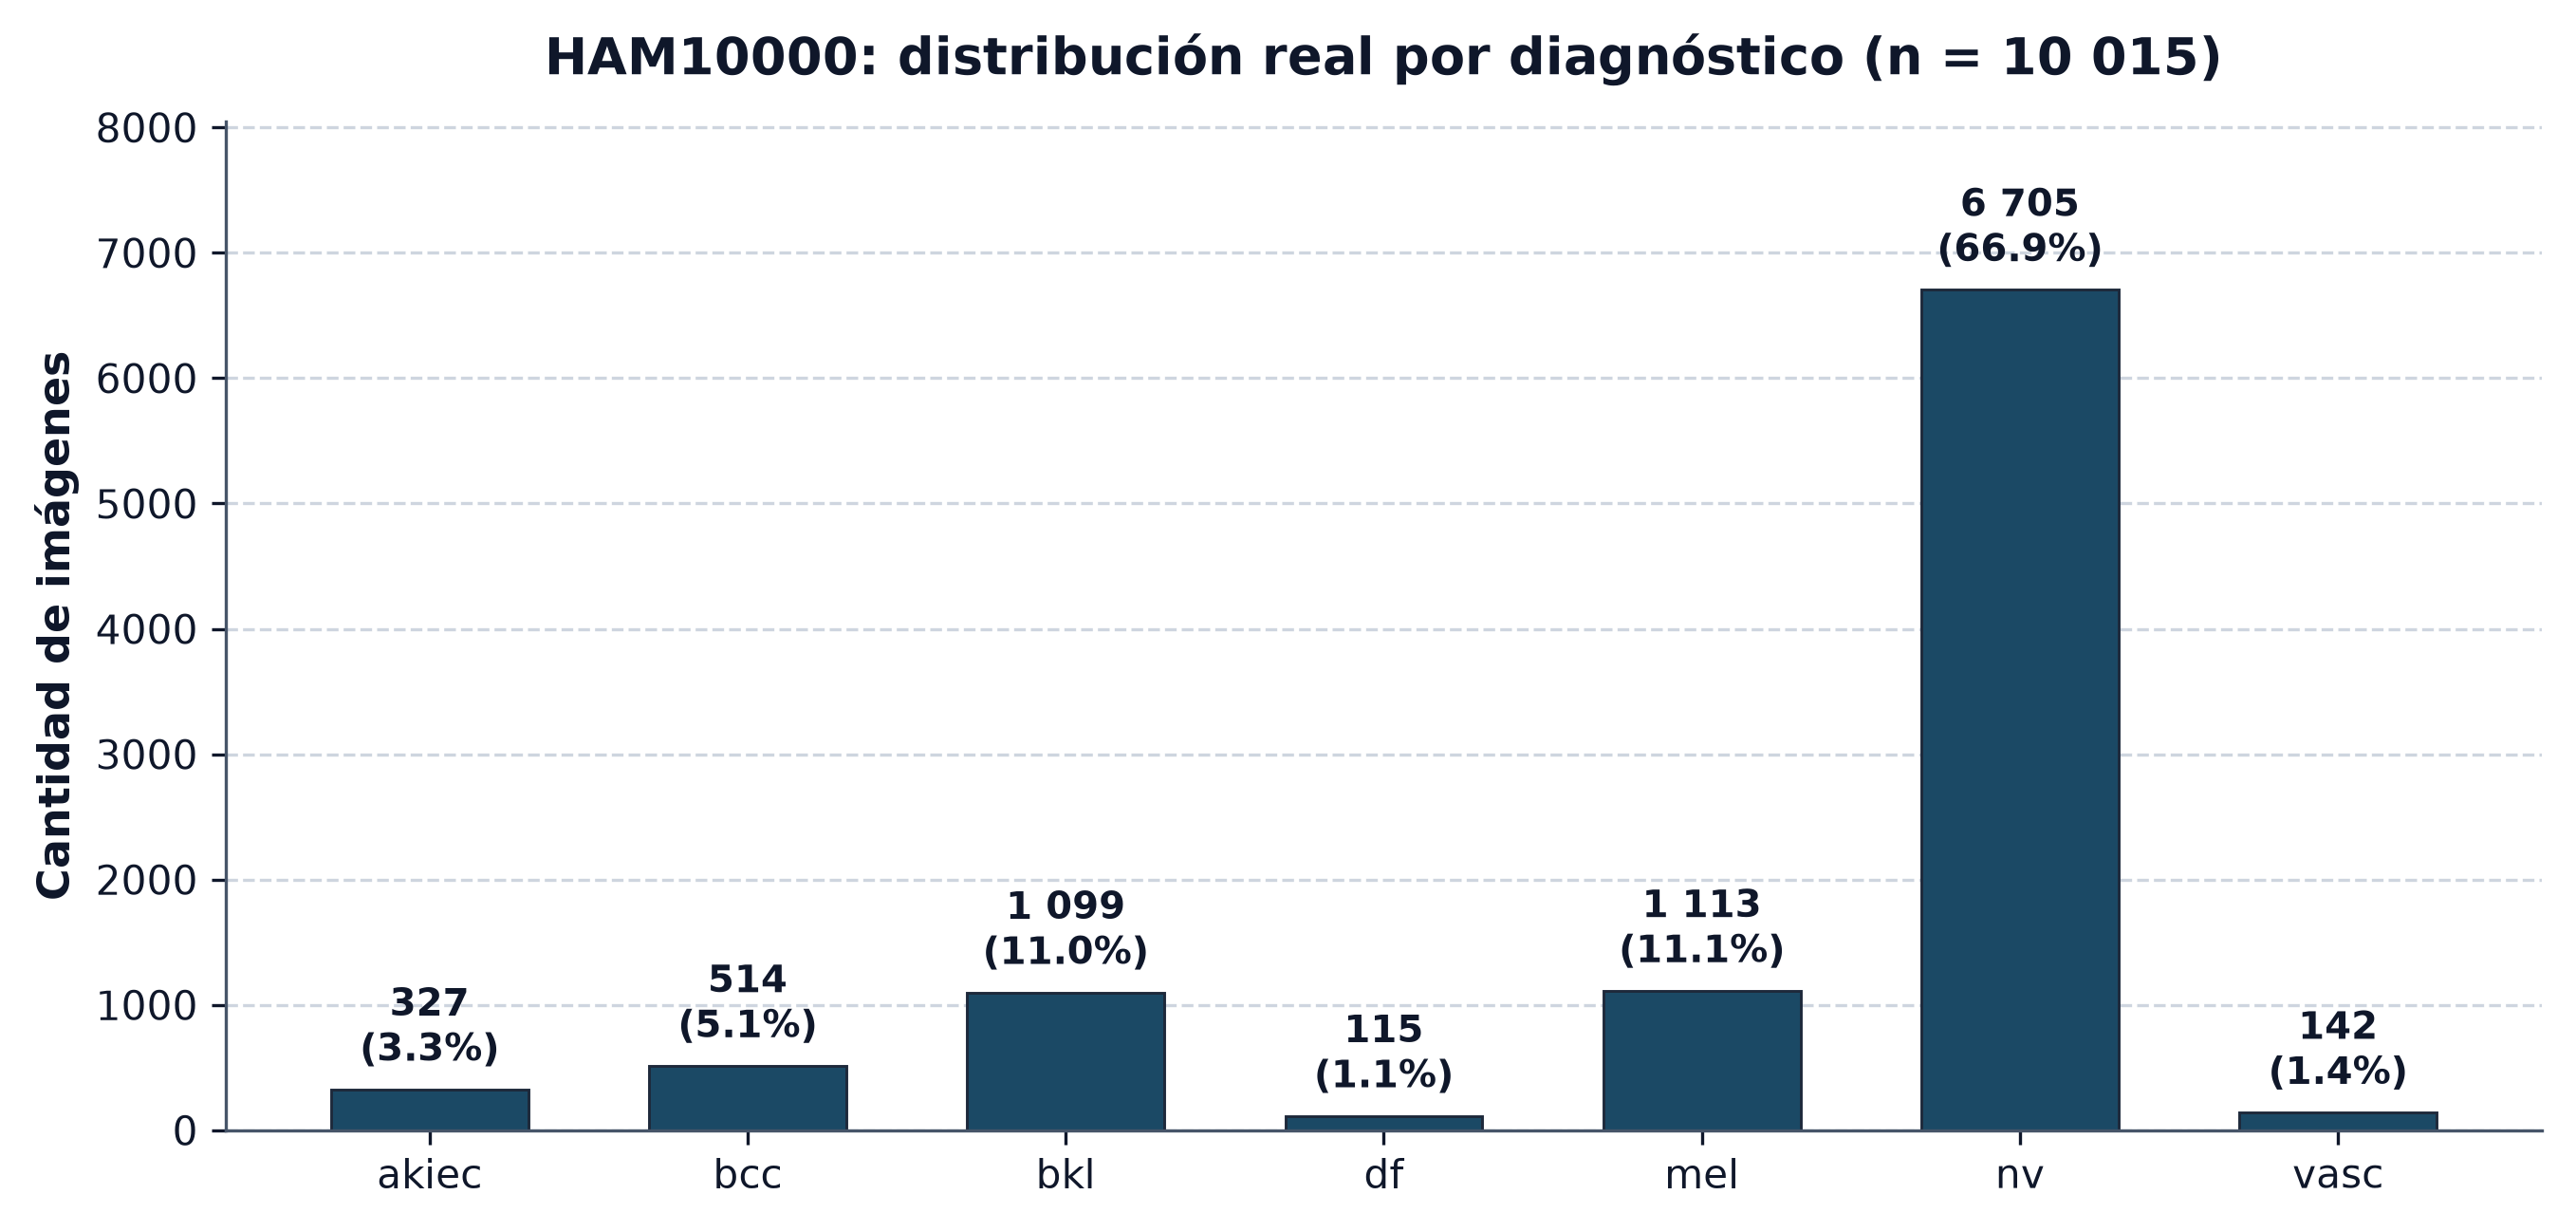
\includegraphics[width=0.92\textwidth]{01_clases.png}
\caption{Conteos y porcentajes reales por clase sobre el metadata local de HAM10000 ($n=10\,015$ imágenes). No representan métricas de desempeño de una CNN.}
\label{fig:clases}
\end{figure}

\begin{figure}[htbp]
\centering
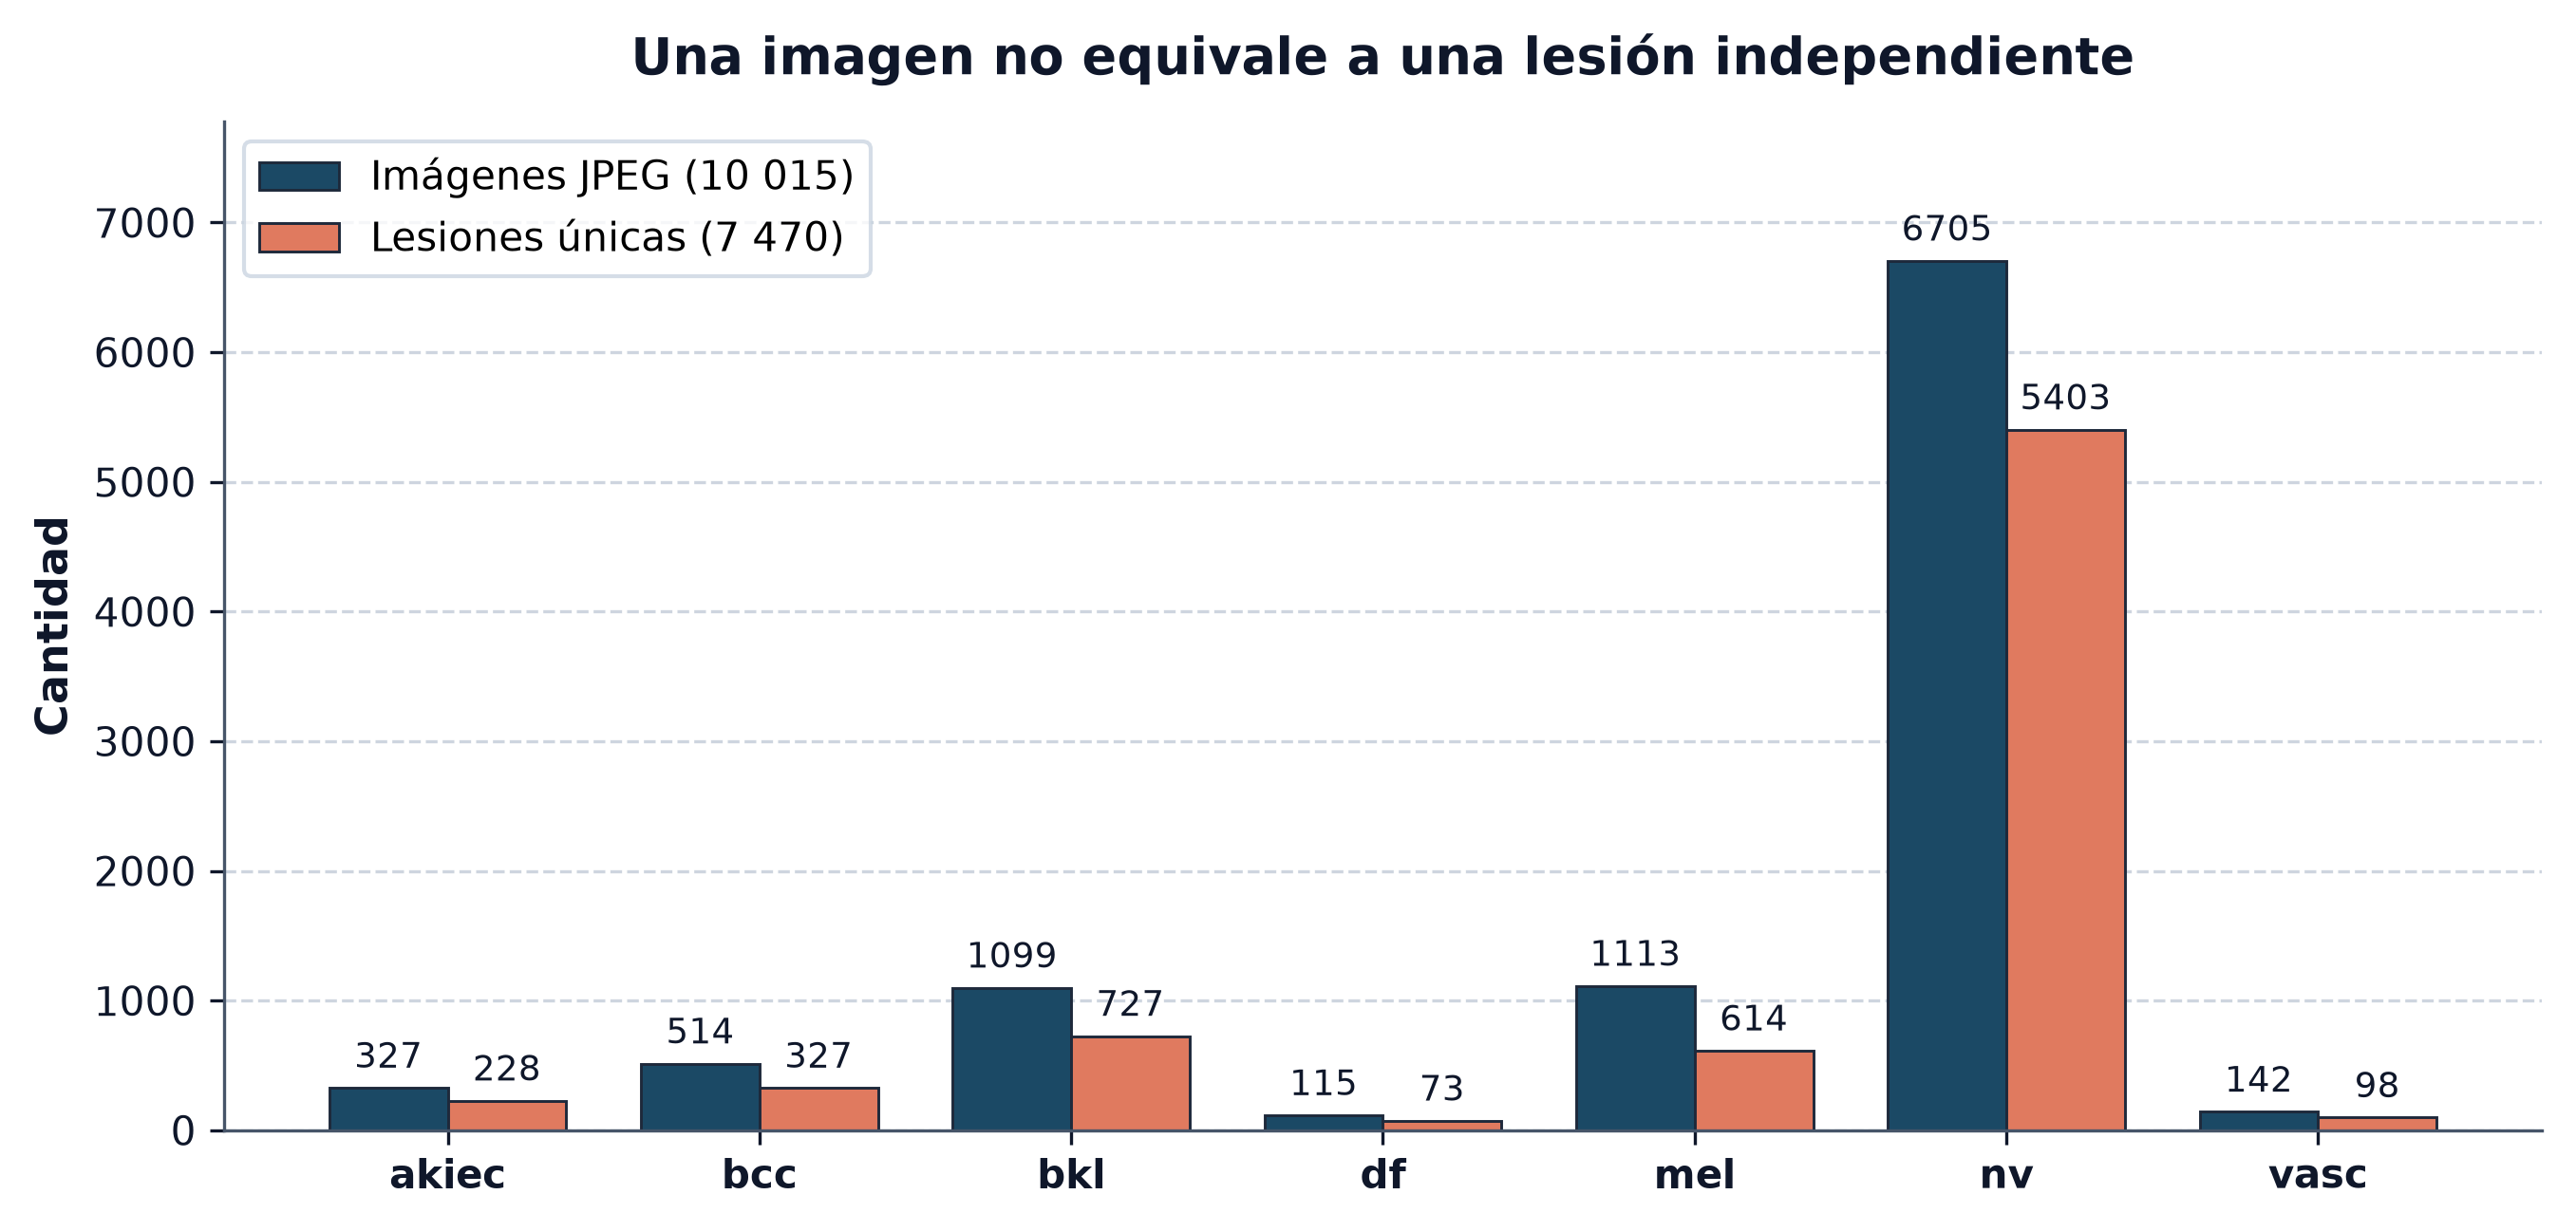
\includegraphics[width=0.92\textwidth]{02_lesiones.png}
\caption{Comparación entre número de imágenes y número de lesiones únicas (\texttt{lesion\_id}, $7\,470$ en total) por categoría diagnóstica en HAM10000.}
\label{fig:lesiones}
\end{figure}

Para ilustrar la variabilidad morfológica de entrada sin exponer muestras de validación ni prueba, la Figura~\ref{fig:muestras} presenta dos ejemplos por categoría pertenecientes exclusivamente al subconjunto de entrenamiento. Se observan diferencias en coloración, bordes, vello y marcas ópticas que justifican un preprocesamiento conservador y evaluación robusta.

\begin{figure}[p]
\centering
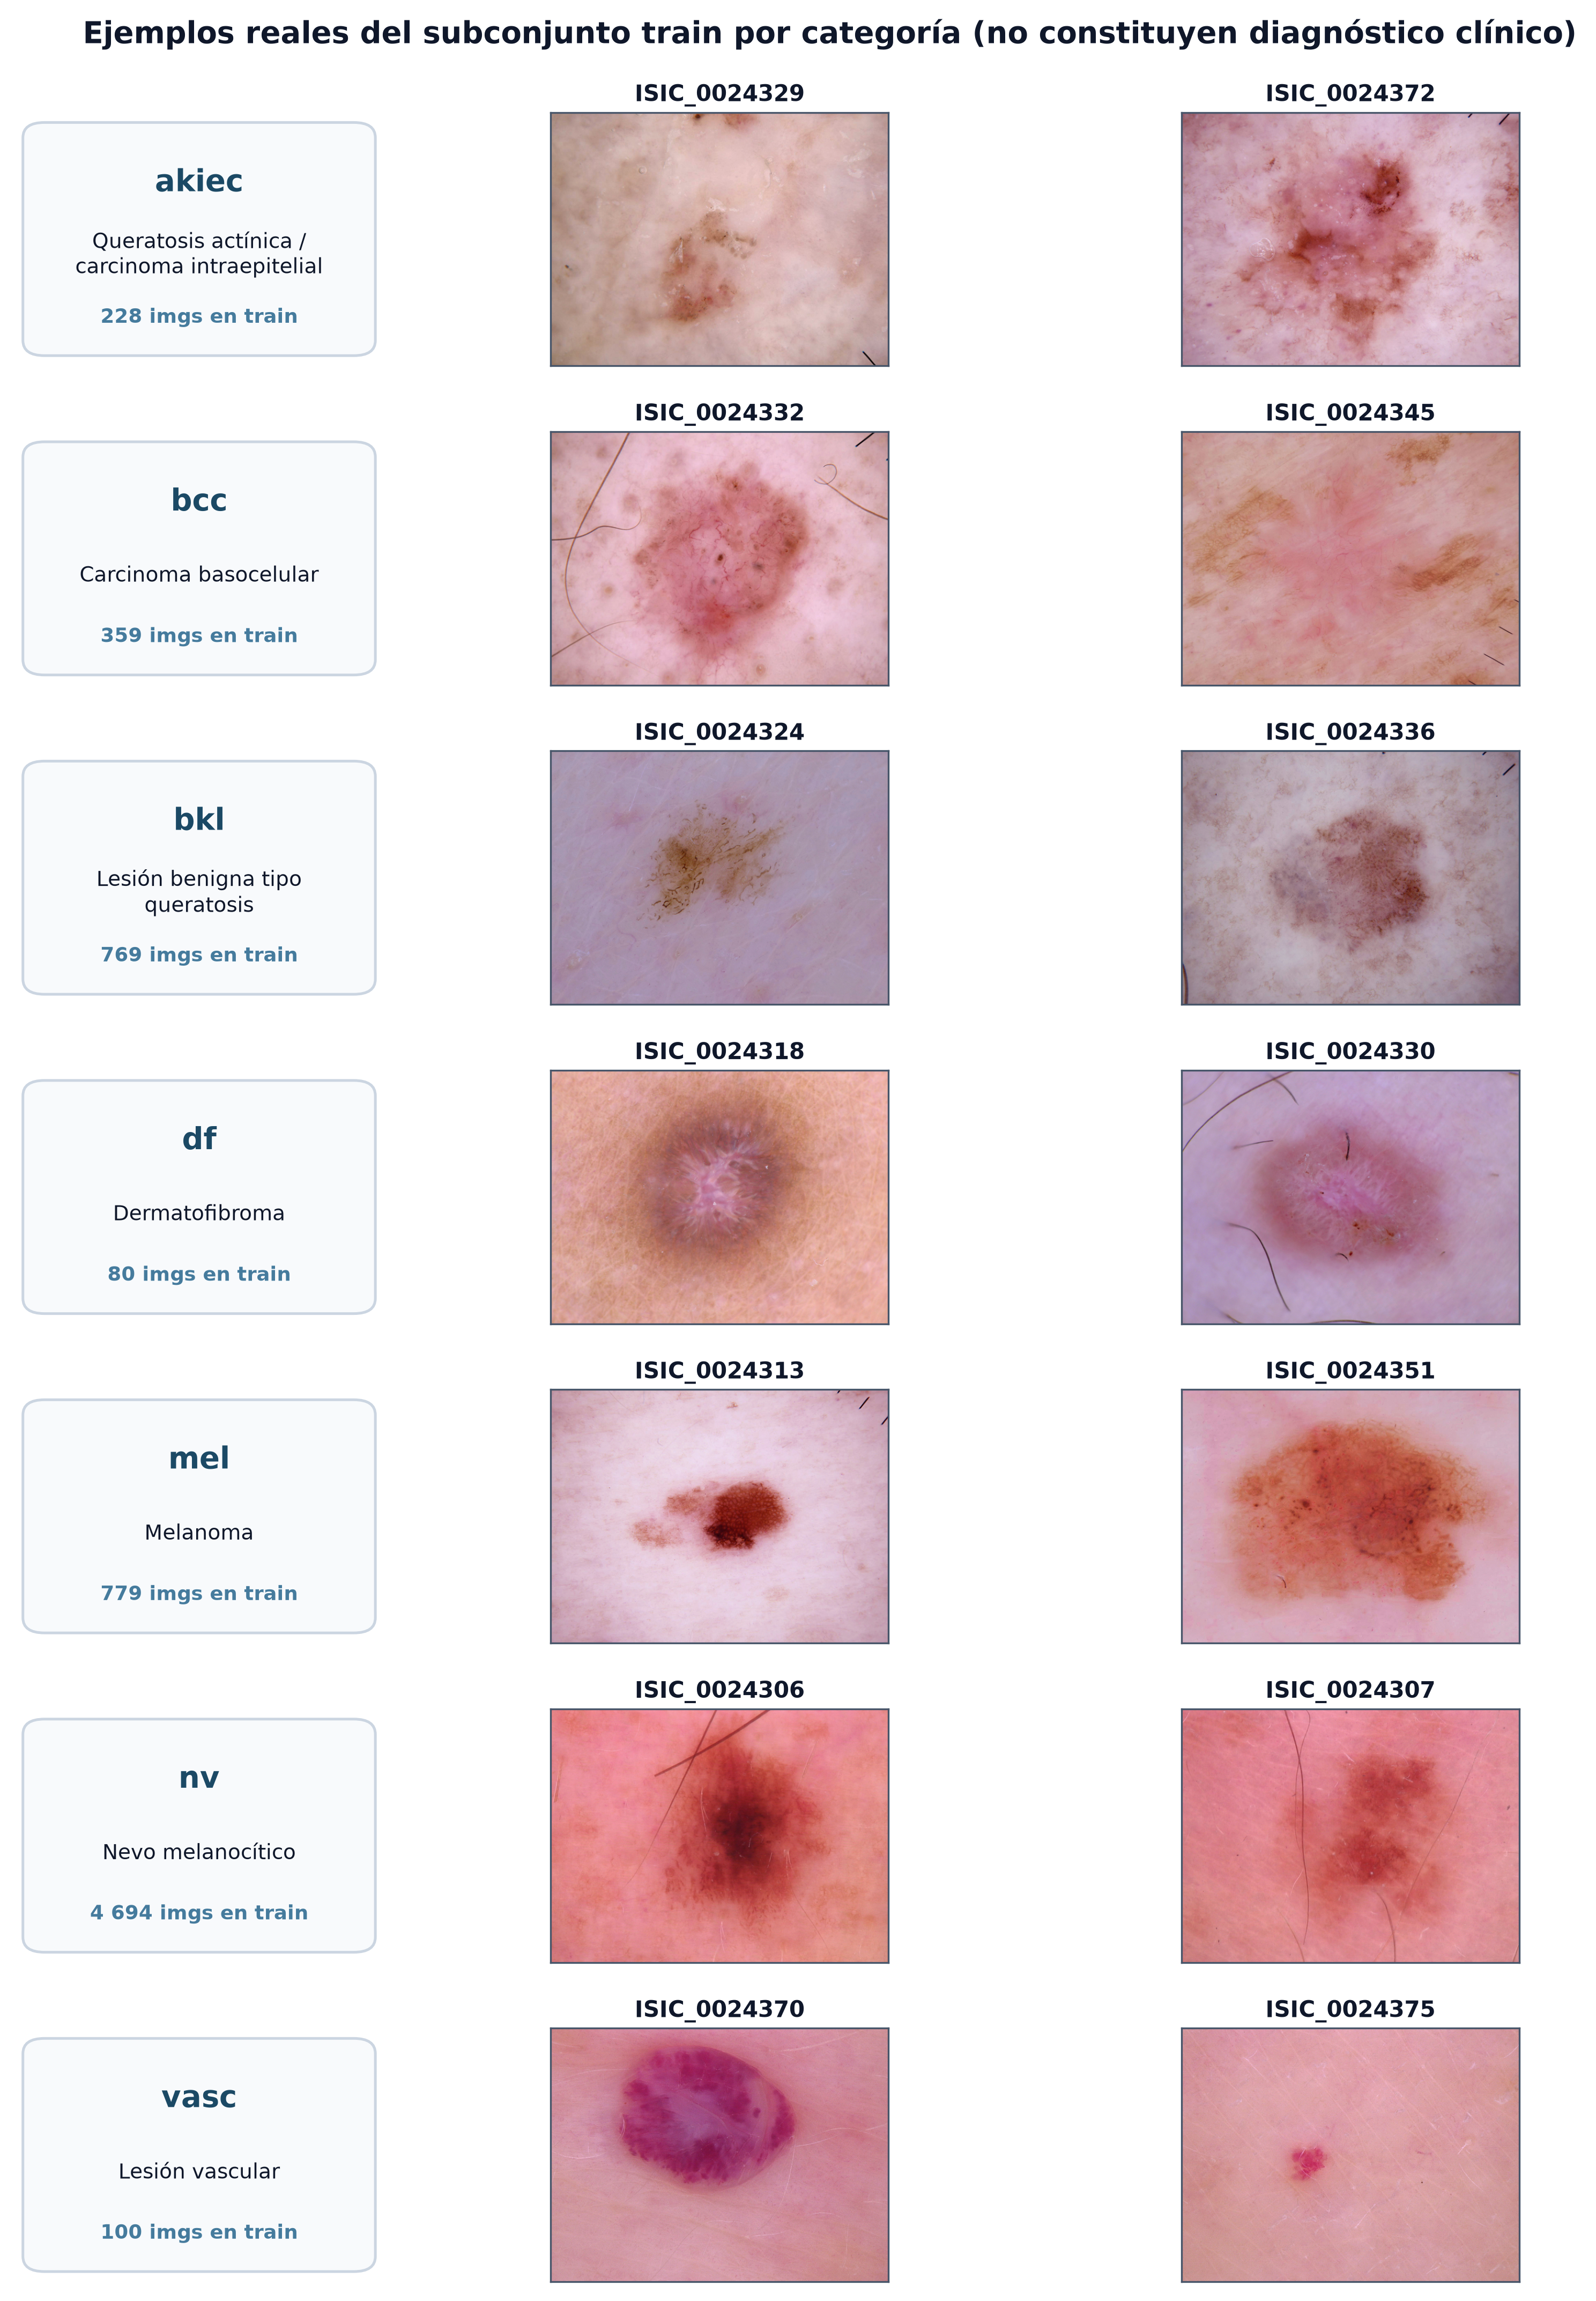
\includegraphics[width=0.94\textwidth,height=0.82\textheight,keepaspectratio]{03_muestras.png}
\caption{Dos ejemplos reales por categoría tomados únicamente de \texttt{train}. La apariencia de una imagen aislada no autoriza un diagnóstico clínico.}
\label{fig:muestras}
\end{figure}

\FloatBarrier
\subsection{Metadatos clínicos y sesgos observables}
Edad, sexo registrado y localización anatómica permiten describir la colección, pero no se utilizan como entradas en la comparación principal. Así se evita introducir una variante multimodal adicional que dificultaría atribuir diferencias de desempeño a la arquitectura visual. Los valores desconocidos o ausentes no se convierten en valores clínicos inventados.

\begin{table}[htbp]\centering\small
\caption{Resumen descriptivo de los metadatos observados en los 10\,015 registros.}
\begin{tabularx}{\textwidth}{@{}>{\bfseries\raggedright\arraybackslash}p{4.0cm}>{\raggedright\arraybackslash}p{5.0cm}>{\raggedright\arraybackslash}X@{}}
\toprule
\textbf{Atributo de metadata} & \textbf{Valores observados} & \textbf{Implicación metodológica} \\ \midrule
Edad (\texttt{age}) & Rango $[0, 85]$ años; media 51.9; 57 ausentes & Contabilizada por imagen; excluye valores faltantes sin imputación clínica. \\
Sexo (\texttt{sex}) & 5\,406 \texttt{male}, 4\,552 \texttt{female}, 57 \texttt{unknown} & Desequilibrio moderado; refleja imágenes registradas, no pacientes únicos. \\
Localización & 15 zonas (\texttt{back}: 2\,192, \texttt{lower ext.}: 2\,077, \texttt{trunk}: 1\,404) & Posible correlación de contexto visual; no se usa como variable auxiliar. \\
Verificación (\texttt{dx\_type}) & \texttt{histo} (5\,340), \texttt{follow\_up} (3\,704), \texttt{consensus} (902), \texttt{confocal} (69) & Las etiquetas no proceden únicamente de biopsia histopatológica. \\
\bottomrule
\end{tabularx}
\end{table}

Los histogramas de las Figuras~\ref{fig:metadata} y~\ref{fig:localizacion} contabilizan imágenes, no sujetos independientes. Una lesión puede contribuir varias veces y el archivo no proporciona un identificador de paciente ni una etiqueta explícita de fototipo cutáneo. La procedencia de la colección y su selección clínica limitan la generalización externa; esa limitación se debe declarar incluso si las métricas internas resultaran altas.

\begin{figure}[htbp]
\centering
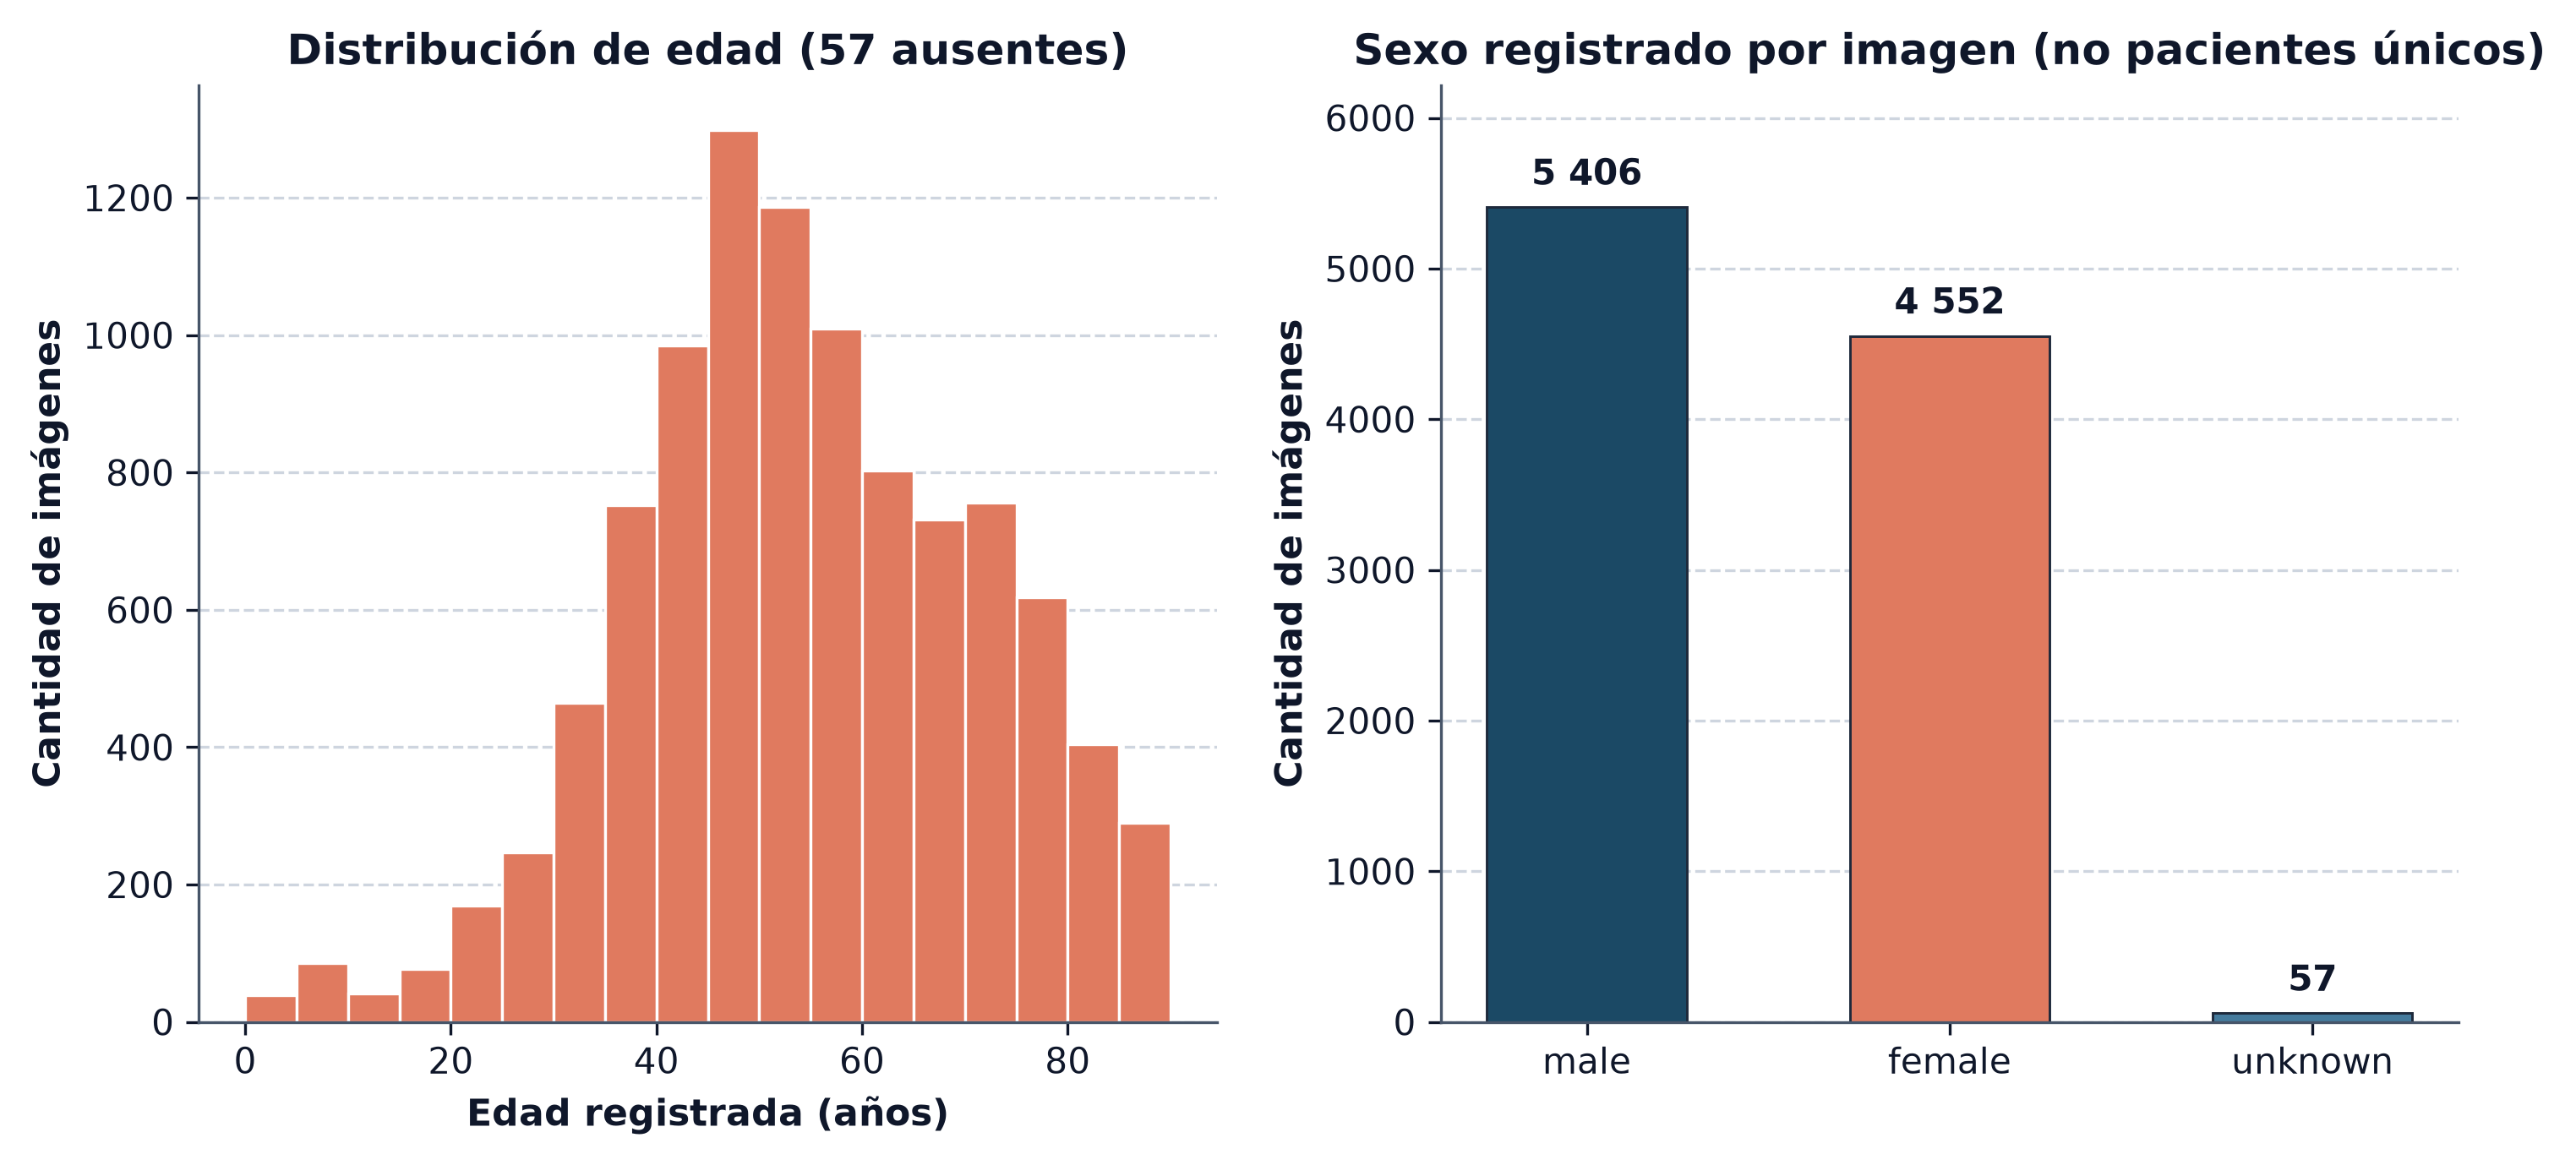
\includegraphics[width=0.92\textwidth]{06_metadata.png}
\caption{Distribución de edad y sexo registrados por imagen en HAM10000, con los 57 datos ausentes señalados explícitamente. Estas variables se describen pero no se añaden al clasificador principal.}
\label{fig:metadata}
\end{figure}

\begin{figure}[htbp]
\centering
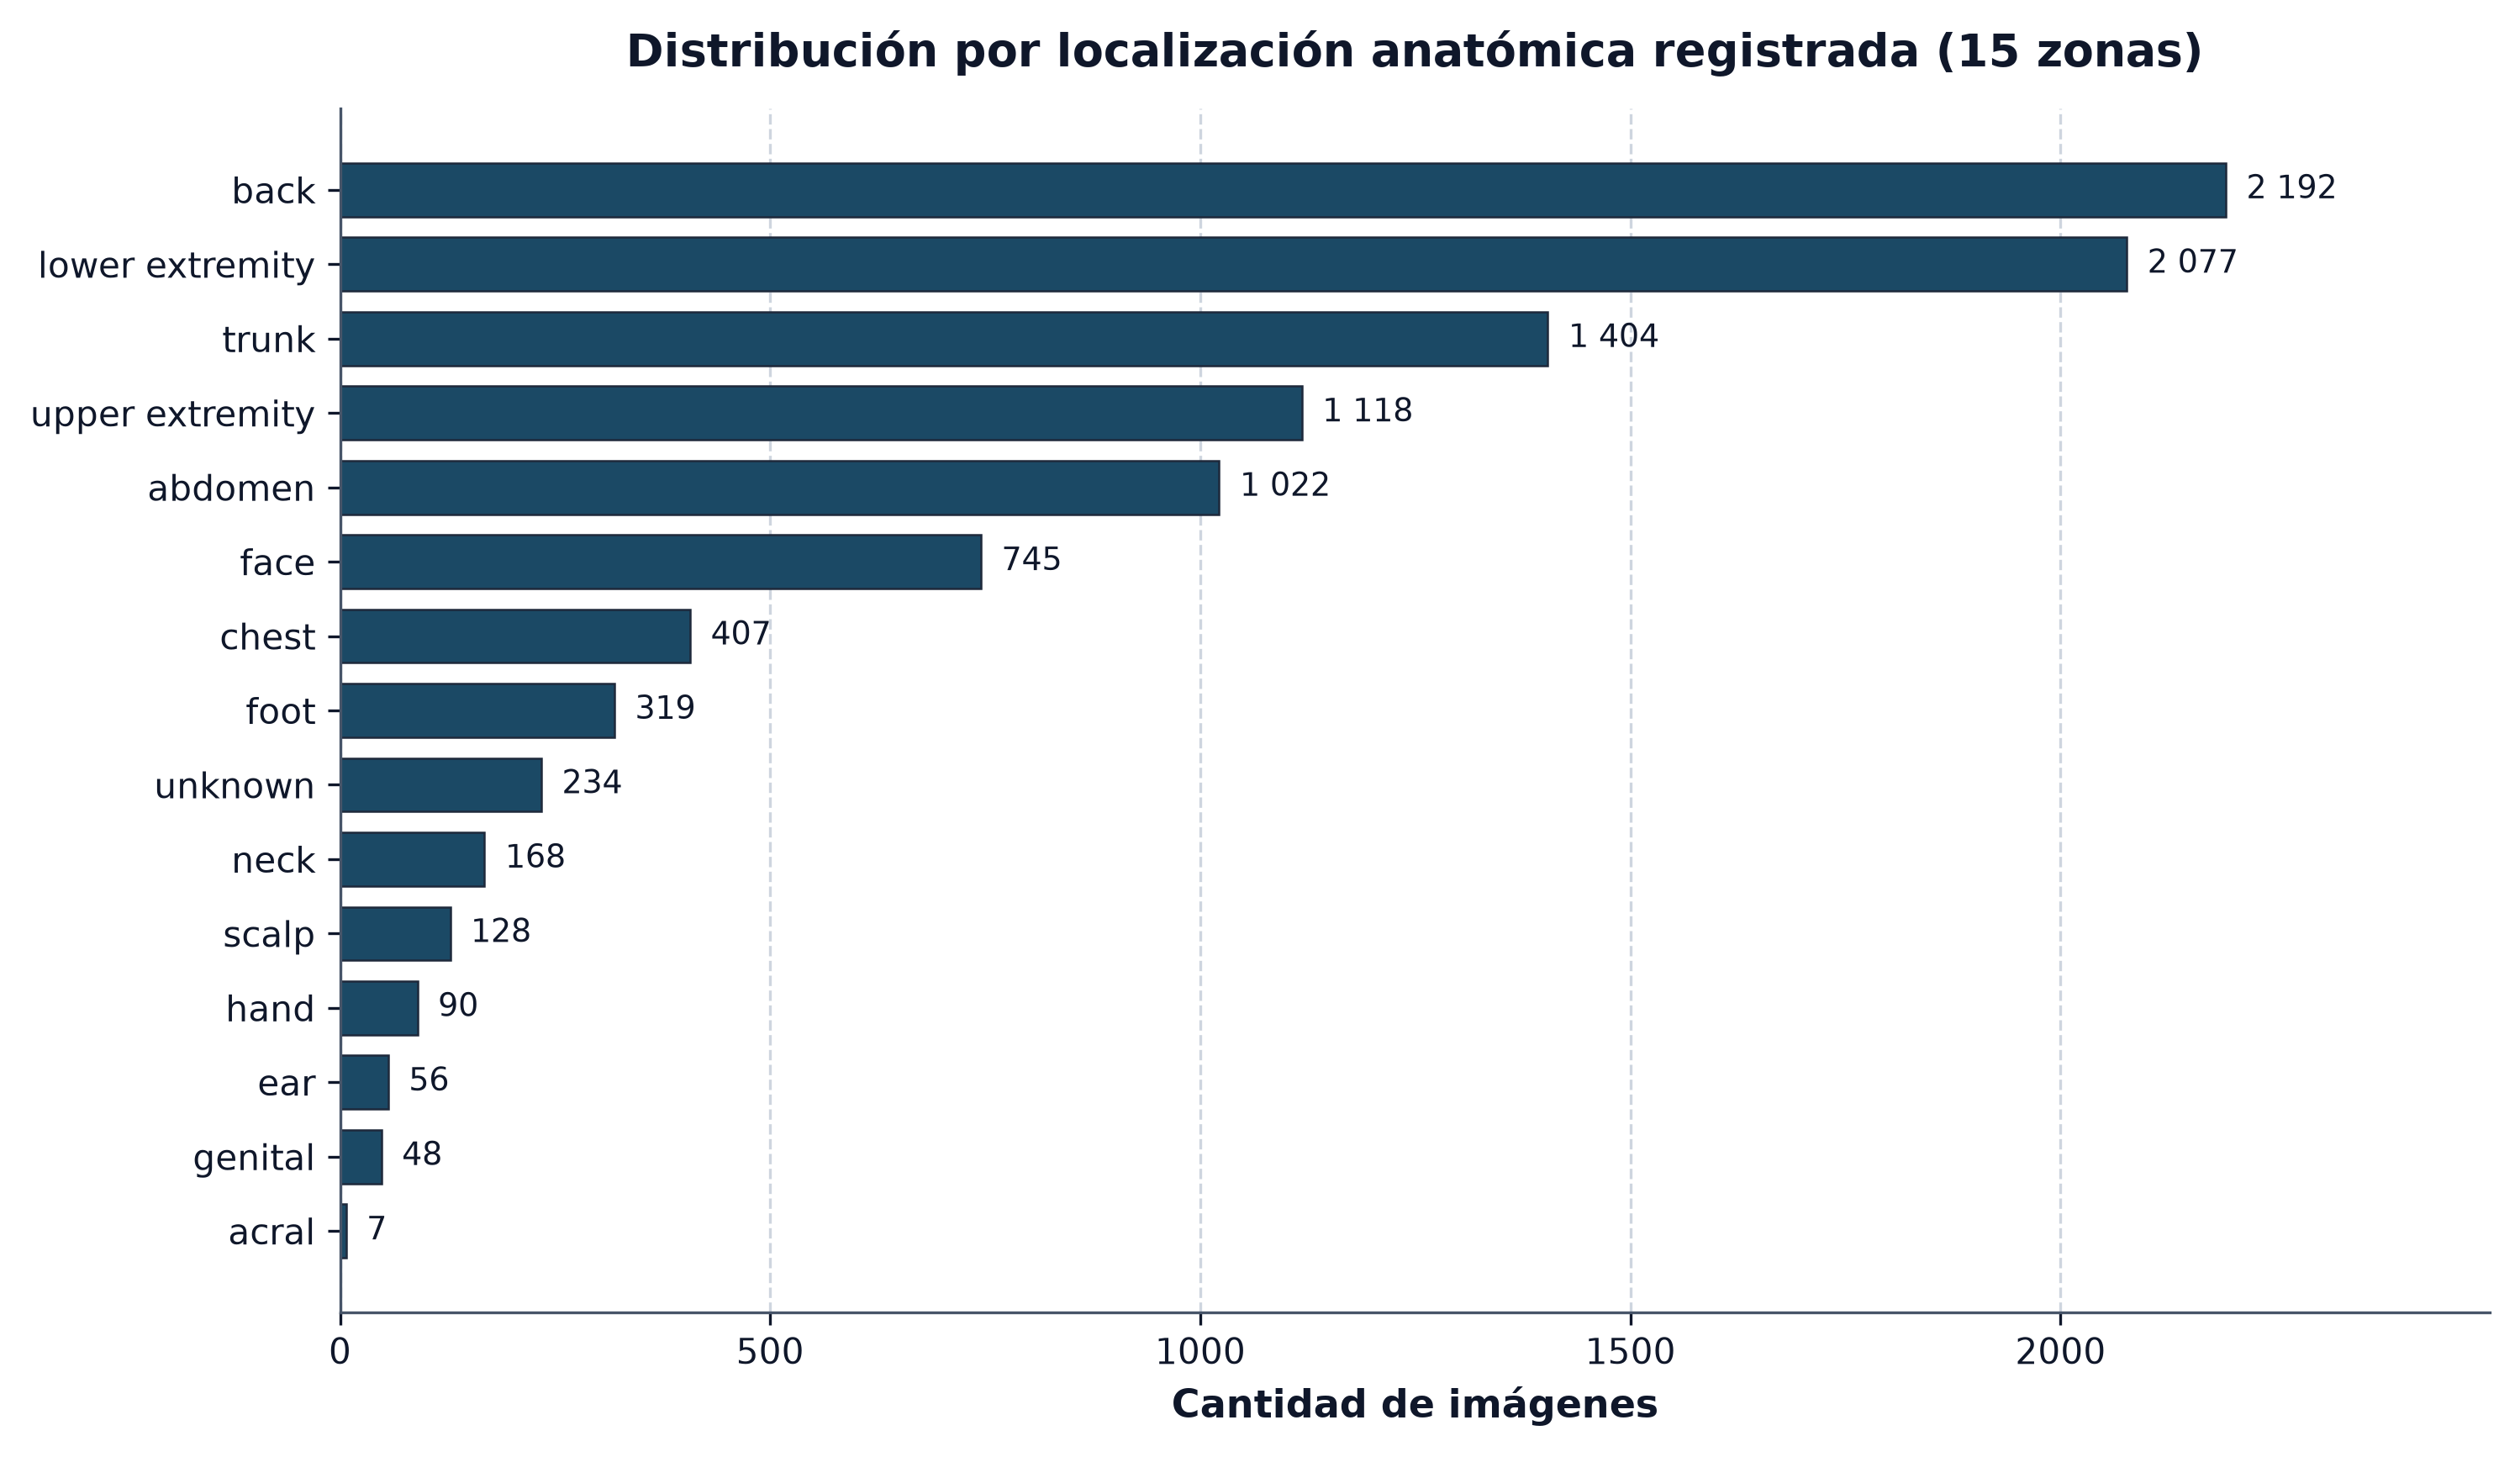
\includegraphics[width=0.92\textwidth]{07_localizacion.png}
\caption{Distribución de localización anatómica en 15 categorías registrada en el metadata de HAM10000 ($n=10\,015$ imágenes). Variable descriptiva no empleada como entrada del clasificador principal.}
\label{fig:localizacion}
\end{figure}
\FloatBarrier

\FloatBarrier\section{Fundamentos de CNN y transferencia de aprendizaje}

\subsection{Qué aprende una red convolucional}
Una CNN es una red neuronal diseñada para procesar datos con estructura espacial. Sus filtros se aplican sobre regiones locales y comparten parámetros a lo largo de la imagen. Esta operación permite detectar patrones sin asignar un conjunto independiente de pesos a cada posición. En capas iniciales pueden aparecer respuestas a bordes, contrastes y texturas; las capas posteriores combinan esas respuestas. Esa descripción es una interpretación funcional, no una garantía de que cada filtro aprenda una característica clínica identificable \cite{goodfellow2016}.

\begin{tcolorbox}[teoriaBox,title={Operación de convolución discreta y proyección multiclase}]
Una convolución espacial bidimensional sobre canales de entrada se formula como:
\begin{equation}
z_{i,j,k}=b_k+\sum_{u,v,c}W_{u,v,c,k}\,x_{i+u,j+v,c}.
\end{equation}
Tras la agregación global espacial, la cabeza lineal produce siete logits $(z_1,\dots,z_7)$ convertidos mediante \textit{softmax}:
\begin{equation}
p_k=\frac{\exp(z_k)}{\sum_{j=1}^{7}\exp(z_j)},\qquad k \in \{1,\dots,7\}.
\end{equation}
\end{tcolorbox}

Los pesos $W$ y sesgos $b$ se ajustan mediante aprendizaje. No se programan manualmente reglas como ``si el borde es irregular entonces melanoma''. Una red puede descubrir correlaciones útiles, pero también atajos espurios. Por eso son esenciales la separación de datos, la revisión de errores y la evaluación fuera de las condiciones de entrenamiento.

\subsection{Del tensor a una distribución de clases}
Cada imagen RGB se representa con tres canales y resolución $224\times224$. La clase predicha se obtiene mediante el argumento máximo de las salidas normalizadas por \textit{softmax}. Estos valores no deben denominarse automáticamente probabilidades clínicas calibradas: una red puede ser demasiado confiada y su calibración requiere una evaluación específica. El reporte guardará las siete salidas por imagen en \texttt{predictions.csv} para permitir auditoría posterior, no solo una etiqueta ganadora.

\subsection{Pérdida, gradiente y actualización}
La entropía cruzada penaliza asignar baja probabilidad a la etiqueta observada. La retropropagación calcula derivadas de la pérdida respecto a los parámetros y el optimizador actualiza los pesos. Una época recorre los lotes del conjunto de entrenamiento; no equivale a una única imagen ni a una ejecución completa del proyecto. El tamaño de lote afecta consumo de memoria y comportamiento de optimización, por lo que debe registrarse.

La pérdida de entrenamiento no es la métrica de prueba. Puede bajar mientras el error en datos no vistos aumenta, fenómeno asociado a sobreajuste. La validación permite detectar ese comportamiento sin utilizar el test como guía. Mirar \texttt{test} repetidamente para escoger una arquitectura o un hiperparámetro transforma indirectamente \texttt{test} en parte del ajuste.

\subsection{Por qué transferencia de aprendizaje}
En lugar de iniciar todos los pesos al azar, se parte de modelos entrenados con ImageNet (\texttt{IMAGENET1K\_V1}). Se sustituye la cabeza original por una salida de siete clases y después se adaptan las representaciones al dominio dermatoscópico. Esta estrategia reduce la necesidad de aprender toda la estructura visual desde una colección relativamente pequeña, aunque no elimina la diferencia entre imágenes naturales y médicas \cite{pan2010}.

El protocolo distingue dos etapas: adaptación inicial de la cabeza y ajuste fino con una tasa menor para el extractor. Congelar un parámetro significa impedir su actualización por gradiente. Además, durante esa etapa deben controlarse los estados de \textit{BatchNorm}; congelar únicamente los pesos no impide que sus estadísticas internas cambien si el módulo permanece en modo de entrenamiento.

\begin{table}[htbp]\centering\small
\caption{Resumen del flujo tensorial y reglas operativas entre etapas del entrenamiento.}
\begin{tabularx}{\textwidth}{@{}>{\bfseries\raggedright\arraybackslash}p{3.6cm}>{\raggedright\arraybackslash}p{4.3cm}>{\raggedright\arraybackslash}X@{}}
\toprule
\textbf{Fase / Módulo} & \textbf{Representación} & \textbf{Comportamiento controlado en código} \\ \midrule
Entrada por lote & Tensor $(B, 3, 224, 224)$ & Normalización ImageNet; en \texttt{train} se descarta último lote incompleto (\texttt{drop\_last=True}). \\
Extractor (\textit{backbone}) & Mapas espaciales + \textit{pooling} & Congelado en épocas 1--2 con \textit{BatchNorm} fijado en \texttt{eval()}; activo en ajuste fino ($\mathrm{lr}=10^{-5}$). \\
Cabeza clasificadora & Vector $(B, d) \to (B, 7)$ & Entrenable desde época 1 ($\mathrm{lr}=10^{-4}$); proyección lineal a las siete categorías. \\
Modo entrenamiento & \texttt{model.train()} selectivo & Gradientes habilitados en capas activas y recorte de norma $L_2 \le 1.0$. \\
Modo evaluación & \texttt{model.eval()} + \texttt{no\_grad} & Congela estadísticas de \textit{BatchNorm} y desactiva \textit{Dropout} en \texttt{val} y \texttt{test}. \\
\bottomrule
\end{tabularx}
\end{table}

\subsection{Entrenamiento y evaluación son modos distintos}
\textit{Dropout} y \textit{BatchNorm} se comportan de manera diferente al entrenar y al inferir. La evaluación debe establecer el modo correspondiente y desactivar el cálculo de gradientes. De lo contrario, una comparación puede resultar inestable o consumir memoria innecesaria. Estas reglas están implementadas en funciones compartidas para evitar diferencias accidentales entre laptop y Colab \cite{pytorch2019,torchvisiondocs}.

Los tres modelos elegidos son CNN, pero no son tres ejecuciones del mismo modelo: cambian sus bloques, conexiones y asignación de capacidad. Compararlos es una comparación válida de arquitecturas profundas para una misma tarea. Cambiar únicamente la semilla produciría repeticiones experimentales, no una arquitectura nueva.

\FloatBarrier\section{Arquitecturas seleccionadas y justificación}

\subsection{ResNet-18 como referencia residual}
ResNet introduce conexiones que suman una transformación aprendida a una ruta de identidad. La formulación básica es $y=F(x)+x$ cuando las dimensiones son compatibles. Si cambian resolución o número de canales, una proyección lineal $W_s x$ ajusta la ruta de atajo. Esta estructura facilita la optimización de redes profundas, pero no significa que toda red más profunda sea mejor para cualquier dataset \cite{he2016}.

ResNet-18 utiliza bloques residuales básicos $3\times 3$ y constituye una referencia ampliamente documentada. En este proyecto interesa porque ofrece una arquitectura suficientemente expresiva sin recurrir de inmediato a una variante mayor. La cabeza original de ImageNet (512 entradas) se reemplaza por una capa lineal de siete salidas, resultando en 11\,180\,103 parámetros reales.

Como hipótesis, la referencia residual puede ofrecer una comparación clara entre capacidad y costo. No se presupone que domine en sensibilidad de melanoma ni en precisión global. La evidencia deberá provenir de la misma partición y receta utilizadas con los otros modelos.

\subsection{EfficientNet-B0 y el equilibrio de recursos}
EfficientNet estudia cómo escalar de forma coordinada la profundidad ($d=\alpha^\phi$), el ancho ($w=\beta^\phi$) y la resolución ($r=\gamma^\phi$) de una familia de redes mediante un coeficiente compuesto $\phi$. B0 es la referencia base de la familia y utiliza bloques invertidos eficientes (\textit{MBConv}) y mecanismos de atención de canales (\textit{Squeeze-and-Excitation}, SE) \cite{tan2019}.

El proyecto no implementa una búsqueda de nuevas arquitecturas ni compara B0 con toda la familia. Utiliza la implementación oficial de TorchVision con pesos \texttt{IMAGENET1K\_V1} y adapta la capa final de su clasificador (\texttt{1280} a \texttt{7} salidas, manteniendo \texttt{Dropout(0.2)}), sumando 4\,016\,515 parámetros totales. El artículo original informa ventajas de eficiencia bajo sus propias condiciones; esas cifras no se trasladan al proyecto como resultados locales sin medición directa.

\subsection{MobileNetV3-Small y la alternativa compacta}
MobileNetV3 combina búsqueda orientada al hardware, bloques invertidos con cuello de botella, convoluciones separables en profundidad, módulos SE y activaciones \textit{hard-swish} en capas profundas \cite{howard2019}. Su variante Small adaptada reemplaza la última capa lineal (\texttt{1024} a \texttt{7} salidas, tras la proyección intermedia $576\to 1024$ con \textit{Hardswish} y \textit{Dropout(0.2)}), sumando 1\,525\,031 parámetros.

La convolución separable divide el filtrado espacial por canal y la combinación puntual $1\times 1$. Esto reduce parámetros y operaciones respecto a una convolución convencional. Sin embargo, el acceso a memoria, el tamaño del lote y la implementación del operador influyen en la latencia real sobre GPU. El experimento debe medir tanto el desempeño diagnóstico como la velocidad real en la misma tarjeta gráfica.

\begin{table}[htbp]\centering\small
\setlength{\tabcolsep}{6pt}
\caption{Especificación técnica y parámetros exactos de las tres CNN adaptadas a siete clases (VRAM sintética con batch 2 a $224\times 224$).}
\begin{tabularx}{\textwidth}{l>{\raggedright\arraybackslash}Xlrr}\toprule
\textbf{Arquitectura} & \textbf{Mecanismo central} & \textbf{Pesos base} & \textbf{Parámetros} & \textbf{VRAM sintética} \\ \midrule
\textbf{ResNet-18} & Bloques residuales $3\times 3$ & \texttt{IMAGENET1K\_V1} & 11\,180\,103 & 147 MiB \\
\textbf{EfficientNet-B0} & MBConv + Squeeze-and-Excitation & \texttt{IMAGENET1K\_V1} & 4\,016\,515 & 208 MiB \\
\textbf{MobileNetV3-Small} & Depthwise separable + SE + h-swish & \texttt{IMAGENET1K\_V1} & 1\,525\,031 & 58 MiB \\
\bottomrule\end{tabularx}\end{table}


\begin{table}[htbp]\centering\footnotesize
\setlength{\tabcolsep}{4.5pt}
\caption{Comparación estructural de bloques, dimensiones de representación y cabezas adaptadas.}
\begin{tabularx}{\textwidth}{@{}>{\bfseries}lccc>{\raggedright\arraybackslash}X@{}}
\toprule
\textbf{Modelo} & \textbf{Activación} & \textbf{Atención SE} & \makecell{\textbf{Dim.\ entrada}\\\textbf{cabeza}} & \textbf{Capa sustituida en \texttt{models.py}} \\ \midrule
ResNet-18 & ReLU & No & 512 & \texttt{fc: Linear(512, 7)} \\
EfficientNet-B0 & SiLU (Swish) & Sí & 1\,280 & \texttt{classifier[-1]: Linear(1280, 7)} \\
MobileNetV3-Small & ReLU / h-swish & Sí & 1\,024 & \texttt{classifier[-1]: Linear(1024, 7)} \\
\bottomrule
\end{tabularx}
\end{table}

\figura{11_arquitecturas.png}{0.98}{Esquema estructural comparativo de las tres CNN adaptadas. Diagrama conceptual de etapas y dimensiones verificadas en \texttt{models.py}.}
\FloatBarrier

\subsection{Condiciones para una comparación justa}
Los tres modelos utilizarán el mismo orden de clases, split, resolución, política de aumento, pérdida, criterio de selección y presupuesto máximo de épocas. Se registran las versiones de los pesos ImageNet, porque ``preentrenado'' no identifica por sí solo una receta. La normalización de canales se mantiene compatible con los pesos, mientras que la geometría común mediante relleno constituye una decisión experimental documentada.

El estudio compara arquitecturas bajo una receta común. No pretende demostrar el óptimo absoluto de cada una, que requeriría búsquedas equivalentes de hiperparámetros y mayor presupuesto. VGG, ResNet-50 o ViT-B/16 no se descartan por ser incorrectos, sino porque no son necesarios para responder la pregunta inicial con cuatro GiB de VRAM. YOLO y U-Net corresponden a otras anotaciones y objetivos; no se incorporan como clasificadores por simple disponibilidad de código.

\FloatBarrier\section{Auditoría, dependencias y partición reproducible}

\subsection{Contrato de entrada y conservación}
La auditoría parte del CSV original y comprueba que cada identificador de imagen tenga un único archivo en los dos lotes esperados. Se comparan los conjuntos de nombres, se leen dimensiones y contenido decodificable, y se calcula SHA-256 de cada JPEG. Un archivo ausente, una etiqueta fuera de la taxonomía o un identificador repetido detienen la preparación; no se corrigen silenciosamente los datos para lograr que el código continúe.

Las imágenes originales permanecen intactas en \texttt{descargaDataSet/HAM10000}. Desde el archivo \texttt{split.csv} se exportan también las carpetas \texttt{train}, \texttt{val} y \texttt{test} por clase ($224\times224$ sin aumento en disco), \texttt{dataset\_procesado.csv} y \texttt{estadisticas.json} calculado exclusivamente sobre entrenamiento. Durante el experimento, el entrenamiento lee directamente los JPEG originales para evitar doble compresión, sin reutilizar aumentos sintéticos como muestras independientes.

\subsection{Imagen, lesión y paciente}
La auditoría confirma 10\,015 imágenes y 7\,470 lesiones únicas (Figura~\ref{fig:lesiones}). Varias imágenes pueden representar la misma lesión bajo distintas condiciones o aumentos ópticos. En concreto, el análisis de multiplicidad muestra que 5\,514 lesiones (73.8\%) tienen una única toma, 1\,423 (19.0\%) tienen dos tomas, 490 (6.6\%) tienen tres, y 43 lesiones reúnen entre cuatro y seis tomas (34 con cuatro, 5 con cinco y 4 con seis). Si una toma se utiliza para aprender y otra para evaluar, la prueba mediría reconocimiento de la lesión ya vista en lugar de generalización. Por ello se agrupa por \texttt{lesion\_id}.

\begin{tcolorbox}[notaBox,title={Alcance de la independencia garantizada}]
No debe afirmarse independencia por paciente. Un paciente podría aportar más de una lesión y \texttt{HAM10000\_metadata.csv} no incluye un identificador de paciente. El nivel de independencia garantizado por este protocolo es el de \texttt{lesion\_id} y duplicados binarios vinculados por SHA-256.
\end{tcolorbox}

\subsection{Duplicados exactos y similitud visual}
Se detectaron dos registros adicionales cuyo contenido binario coincide exactamente con otro JPEG indexado (\texttt{ISIC\_0024366}/\texttt{ISIC\_0029861} en \texttt{HAM\_0002300} y \texttt{ISIC\_0024777}/\texttt{ISIC\_0029938} en \texttt{HAM\_0001895}, ambos en la clase \texttt{nv}). Se conservan por trazabilidad y quedan confinados en el mismo grupo mediante \textit{Union-Find} (registrado en \texttt{auditoria.json}). Adicionalmente, en una comprobación puntual de sesión (sin script ni reporte independiente persistido en el repositorio), un barrido por parejas sobre miniaturas RGB $16\times 12$ entre todas las muestras con distinto \texttt{lesion\_id} encontró cero pares con $\mathrm{RMSE}<4.5$.

SHA-256 y la comparación de baja resolución descartan igualdad de bytes y copias casi idénticas directas, pero no reemplazan una revisión dermatológica especializada de similitud visual. La documentación y \texttt{auditoria.json} mantienen esta limitación perceptual de forma transparente.

\subsection{Construcción del split fijo}
Se utiliza \texttt{StratifiedGroupKFold} con veinte pliegues, mezcla reproducible y semilla 42. Los pliegues cero a dos forman \texttt{test}; los tres a cinco forman \texttt{val}; los catorce restantes forman \texttt{train}. La estratificación conserva proporciones de clase mientras el agrupamiento mantiene las dependencias juntas \cite{sklearndocs}.

Esta construcción produce aproximadamente 70/15/15, sin prometer porcentajes exactos por imagen porque los grupos no pueden fraccionarse. Los resultados reales son 7\,009 imágenes en \texttt{train} (69.99\%), 1\,503 en \texttt{val} (15.01\%) y 1\,503 en \texttt{test} (15.01\%). La misma asignación se reutiliza en las tres CNN y en Colab. La referencia 80/20 mencionada en orientaciones generales se interpreta como referencial; cualquier otro reparto exigiría fijar un nuevo protocolo antes de experimentar.

\begin{table}[htbp]\centering\normalsize
\setlength{\tabcolsep}{8pt}
\caption{Conteos reales de la partición fija libre de fuga (\textasciitilde 70/15/15) y pesos de clase en entrenamiento.}
\begin{tabularx}{\textwidth}{>{\raggedright\arraybackslash}Xrrrr}\toprule
\textbf{Clase} & \textbf{Train} & \textbf{Val} & \textbf{Test} & \textbf{Peso $w_c$} \\ \midrule
\texttt{akiec} & 228 & 50 & 49 & 4.3916 \\
\texttt{bcc} & 359 & 77 & 78 & 2.7891 \\
\texttt{bkl} & 769 & 165 & 165 & 1.3021 \\
\texttt{df} & 80 & 18 & 17 & 12.5161 \\
\texttt{mel} & 779 & 166 & 168 & 1.2853 \\
\texttt{nv} & 4\,694 & 1\,006 & 1\,005 & 0.2133 \\
\texttt{vasc} & 100 & 21 & 21 & 10.0129 \\
\midrule
\textbf{Total} & \textbf{7\,009} & \textbf{1\,503} & \textbf{1\,503} & --- \\
\bottomrule\end{tabularx}\end{table}


\begin{figure}[htbp]
\centering
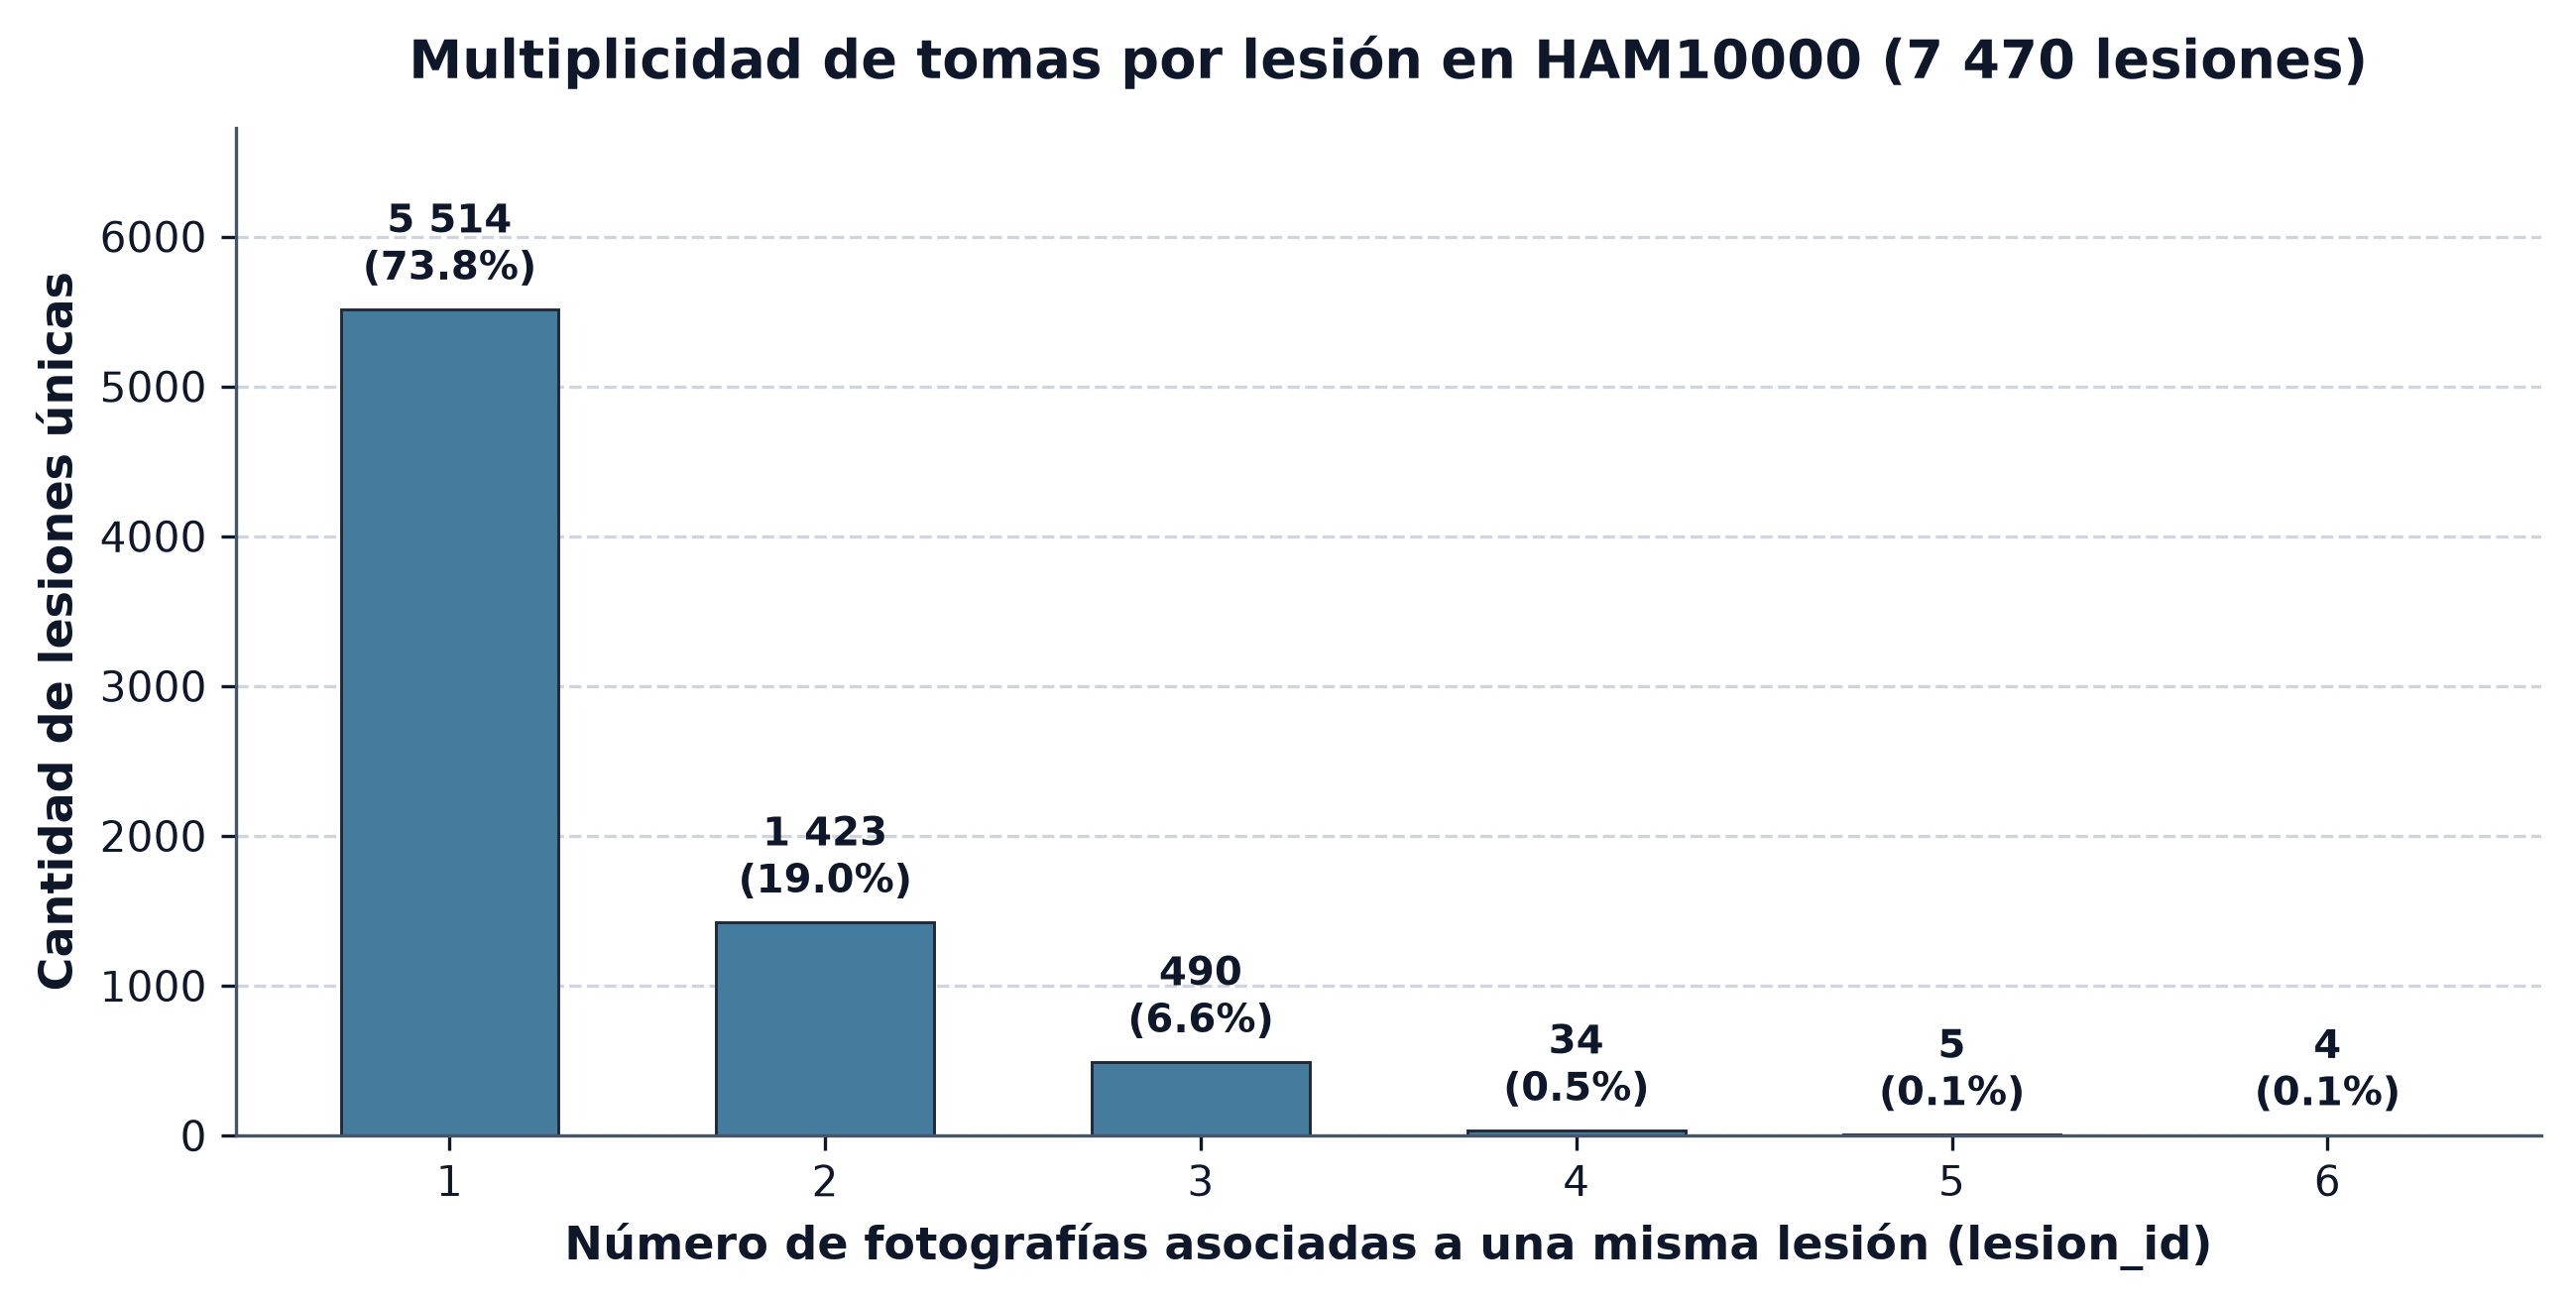
\includegraphics[width=0.92\textwidth]{05_multiplicidad.png}
\caption{Número de imágenes por lesión única (\texttt{lesion\_id}) en HAM10000 (26.2\% de las lesiones presentan múltiples tomas).}
\label{fig:multiplicidad}
\end{figure}

\begin{figure}[htbp]
\centering
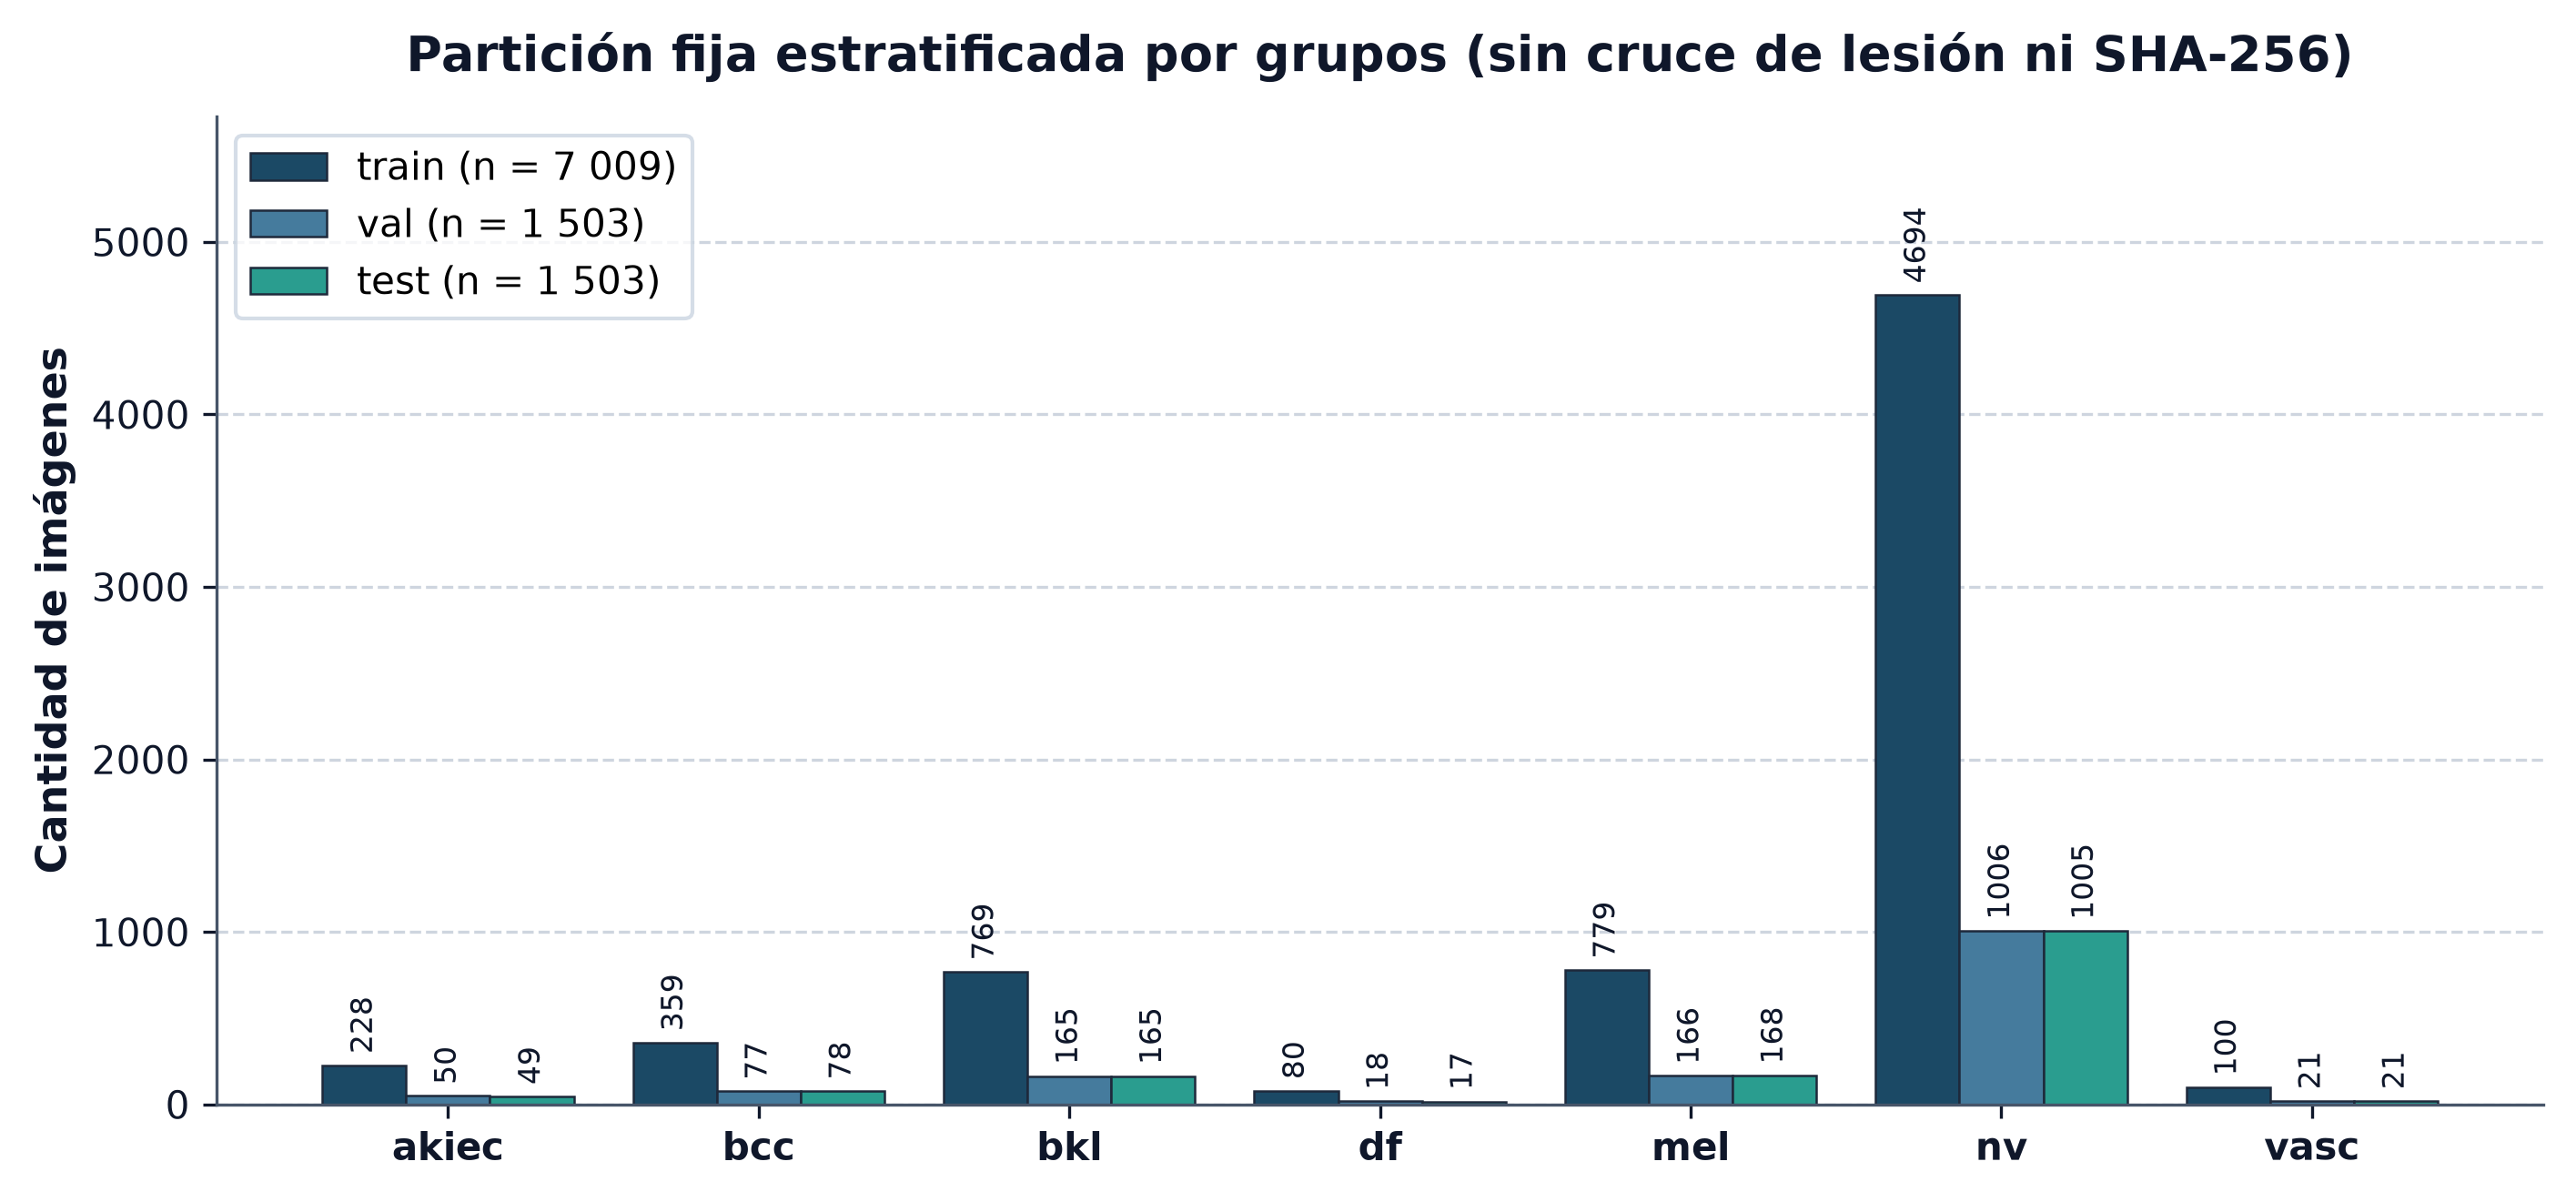
\includegraphics[width=0.92\textwidth]{04_split.png}
\caption{Conteos reales del split fijo por categoría diagnóstica en \texttt{train}, \texttt{val} y \texttt{test} tras agrupar por lesión y SHA-256 sin fugas.}
\label{fig:split}
\end{figure}
\FloatBarrier

\subsection{Pruebas automáticas de integridad y control criptográfico}
El programa verifica ausencia de cruce de \texttt{lesion\_id}, \texttt{group\_id} y SHA-256 entre particiones, exige presencia de todas las clases y conserva la huella del CSV completo. Los checkpoints guardan esa huella y rechazan una reanudación o evaluación con otro manifiesto. Al trasladar el proyecto a Colab se validan los 10\,015 archivos frente al mismo manifiesto sin volver a sortear el split.

\begin{table}[htbp]\centering\small
\caption{Resumen de verificaciones de integridad y control antifuga ejecutadas sobre \texttt{split.csv}.}
\begin{tabularx}{\textwidth}{@{}>{\bfseries\raggedright\arraybackslash}p{4.6cm}>{\raggedright\arraybackslash}p{4.6cm}>{\raggedright\arraybackslash}X@{}}
\toprule
\textbf{Comprobación} & \textbf{Resultado verificado} & \textbf{Mecanismo en \texttt{prepare.py} / \texttt{io.py}} \\ \midrule
Integridad archivo--metadata & 10\,015 / 10\,015 JPEG válidos & Verificación de lectura, dimensiones $600\times450$ y SHA-256. \\
Duplicados binarios exactos & 2 pares en \texttt{nv} confinados & Agrupación \textit{Union-Find} por \texttt{lesion\_id} + SHA-256 (7\,470 grupos). \\
Casi-duplicados entre lesiones & 0 pares con $\mathrm{RMSE} < 4.5$ (sesión) & Comprobación puntual de sesión en RGB $16\times12$ (sin reporte independiente; limitación perceptual vigente en \texttt{auditoria.json}). \\
Cruce entre subconjuntos & 0 intersecciones en 3 ejes & Aserciones de disjunción por lesión, grupo y SHA-256. \\
Inmutabilidad del manifiesto & \texttt{583779fb75f28758...} & Comprobación estricta de \texttt{split\_sha256} al reanudar o evaluar. \\
\bottomrule
\end{tabularx}
\end{table}
\FloatBarrier

\FloatBarrier\section{Preprocesamiento y aumento de datos}

\subsection{Un pipeline compartido}
El preprocesamiento establece cómo una fotografía se convierte en el tensor de entrada de la red. La misma función base se reutiliza en entrenamiento, validación y prueba para evitar discrepancias entre fases. El aumento aleatorio se añade exclusivamente a \texttt{train}. No se exportan imágenes aumentadas antes de separar las muestras: hacerlo podría introducir versiones de una misma imagen en conjuntos distintos.

La implementación utiliza Pillow para lectura y conversión a RGB. Se atiende la orientación EXIF si está disponible y se mantienen tres canales. El orden de canales debe ser explícito; cargar una imagen BGR y tratarla como RGB alteraría los colores sin necesariamente producir un error de ejecución.

\subsection{Geometría sin deformar la lesión}
La entrada común es de $224\times224$ píxeles. Se redimensiona conservando la proporción (\textit{letterbox} bilineal) y se centra la imagen sobre un lienzo cuadrado. Esta operación evita estirar de forma distinta los ejes y, a diferencia de un recorte central, no elimina deliberadamente la periferia para obtener el cuadrado. El relleno usa un color asociado a la media de normalización de ImageNet.

\figura{08_preprocesamiento.png}{1.0}{Ejemplo real de \texttt{train}: original ($600\times450$), adaptación geométrica (\textit{letterbox} $224\times224$) y aumento determinista. La normalización se deshace únicamente para visualizar el tercer panel.}

\subsection{Escalado y normalización}
Los valores se transforman a un tensor flotante y se escalan al rango $[0,1]$. Después se normalizan por canal:
\begin{equation}
x'_c=\frac{x_c-\mu_c}{\sigma_c},\qquad
\mu=(0.485,0.456,0.406),\quad
\sigma=(0.229,0.224,0.225).
\end{equation}
Estos valores corresponden al esquema de normalización de los pesos ImageNet seleccionados. De manera complementaria, el archivo \texttt{estadisticas.json} registra las estadísticas empíricas calculadas estrictamente sobre los 7\,009 ejemplos de entrenamiento ($\mu_{\mathrm{train}}=[0.693823, 0.523161, 0.529890]$, $\sigma_{\mathrm{train}}=[0.170584, 0.136846, 0.162109]$) \cite{torchvisiondocs}.

\subsection{Aumento moderado y política reproducible}
Se permiten volteos horizontal y vertical ($p=0.5$), rotación de hasta $\pm 30^\circ$ y cambios moderados de brillo y contraste entre $0.9$ y $1.1$. El propósito es reducir dependencia de variaciones de adquisición sin borrar características clínicas relevantes. El estado aleatorio del aumento se deriva mediante SHA-256 de la semilla, la época y el identificador de imagen, asegurando que las arquitecturas compitan bajo exactamente la misma secuencia de aumentos.

\begin{table}[htbp]\centering\small
\caption{Especificación exacta de transformaciones por partición implementada en \texttt{data.py}.}
\begin{tabularx}{\textwidth}{@{}>{\bfseries\raggedright\arraybackslash}p{4.1cm}cc>{\raggedright\arraybackslash}X@{}}
\toprule
\textbf{Operación} & \textbf{\texttt{train}} & \textbf{\texttt{val / test}} & \textbf{Parámetros e implementación} \\ \midrule
Lectura y orientación & Sí & Sí & Apertura desde JPEG original vía \texttt{ImageOps.exif\_transpose} en RGB. \\
Adaptación geométrica & Sí & Sí & \textit{Letterbox} bilineal isotrópico a $224\times224$ con relleno media ImageNet. \\
Volteo horizontal / vertical & Sí & No & Probabilidad $p=0.5$ independiente por eje con generador determinista. \\
Rotación aleatoria & Sí & No & Ángulo uniforme en $[-30^\circ, +30^\circ]$, interpolación bilineal y relleno media. \\
Brillo y contraste & Sí & No & Factores independientes uniformes en $[0.9, 1.1]$. \\
Perturbación de robustez & No & Configurable & Solo en evaluación (\texttt{clean}, \texttt{noise\_002/005}, \texttt{blur\_1/2}). \\
Normalización de tensor & Sí & Sí & Conversión a $[0,1]$ y estandarización ImageNet ($\mu,\sigma$). \\
\bottomrule
\end{tabularx}
\end{table}

\subsection{Qué no se aplica por defecto}
La eliminación de vello, CLAHE y filtros de suavizado no se consideran mejoras universales: pueden reducir artefactos, pero también alterar bordes o pigmentación. Si se evalúa alguna variante, sus parámetros deberán seleccionarse en validación y aplicarse por igual a todos los modelos.
\FloatBarrier

\FloatBarrier\section{Entorno local, instalación y comprobación de GPU}

\subsection{Hardware disponible}
La laptop inspeccionada es una Acer Nitro AN515-45 con procesador AMD Ryzen 5 5600H, seis núcleos y doce hilos, aproximadamente 24~GB de memoria instalada y GPU NVIDIA GeForce GTX 1650 de cuatro GiB. También dispone de gráficos integrados AMD. La presencia de dos adaptadores no indica un fallo; en una laptop híbrida cumplen funciones distintas.

La RAM del sistema y la VRAM no son intercambiables a efectos de capacidad de un lote de entrenamiento. La memoria debe medirse en el dispositivo gráfico realmente utilizado. Por ese motivo se comienza con batch pequeño y resolución moderada, ejecutando un piloto antes de fijar los tiempos finales.

\subsection{Diagnóstico inicial y corrección}
La inspección inicial encontró PyTorch \texttt{2.15.0+cpu} en el Python global de Laragon. Esa distribución no incluía CUDA, aunque la GPU estaba reconocida y el controlador podía inicializarse. Se comprobó el instalador Notebook 621.01 en la página oficial de NVIDIA \cite{nvidiadriver,acerdrivers}, verificando firma e integridad frente al paquete oficial. Tras su instalación, el controlador confirmó versión 621.01 e inicialización CUDA correcta.

\subsection{Entorno aislado del proyecto}
Se creó un entorno virtual \texttt{.venv} independiente del Python global. Se instalaron las bibliotecas con CUDA: PyTorch versión \texttt{2.11.0+cu128} y torchvision versión \texttt{0.26.0+cu128}. El soporte compilado incluye la arquitectura \texttt{sm\_75} de la GTX 1650. La descarga inicial fue de aproximadamente 2.79~GB decimales e incluye bibliotecas de ejecución, sin requerir instalación separada del CUDA Toolkit completo.

El paquete portable conserva \texttt{python/requirements-cuda.txt}, \texttt{requirements-common.txt} y requisitos opcionales de notebook. El kernel local debe apuntar al intérprete del entorno correcto; el cuaderno imprime su ruta antes de importar dependencias. En Colab se conserva el PyTorch compatible del runtime y se registran sus versiones, sin instalar la wheel de Windows ni su controlador.

\begin{table}[htbp]\centering\small
\caption{Entorno de cómputo y verificaciones locales efectivamente observadas.}
\begin{tabularx}{\textwidth}{@{}>{\bfseries\raggedright\arraybackslash}p{4.8cm}>{\raggedright\arraybackslash}X@{}}
\toprule
\textbf{Elemento del entorno} & \textbf{Estado verificado localmente} \\ \midrule
Equipo y CPU & Laptop Acer Nitro AN515-45, AMD Ryzen 5 5600H (6 núcleos / 12 hilos), 24~GB RAM \\
Sistema operativo & Windows 11 Pro de 64 bits \\
Controlador NVIDIA & Versión 621.01 WHQL (firma e integridad verificadas) \\
GPU dedicada & NVIDIA GeForce GTX 1650, capacidad de cómputo 7.5 (\texttt{sm\_75}), 4\,096 MiB VRAM \\
Intérprete aislado & Python 3.12.8 en \texttt{.venv} (sin alterar el Python global de Laragon) \\
PyTorch / torchvision & \texttt{2.11.0+cu128} / \texttt{0.26.0+cu128} \\
Prueba matricial CUDA & Multiplicación tensorial ejecutada y verificada en \texttt{cuda:0} \\
Tres CNN, batch 2, 224 px & \textit{Forward/backward} sintético OK: 147 / 208 / 58 MiB de pico asignado \\
Integridad de paquetes & \texttt{pip check}: sin dependencias rotas ni conflictos \\
\bottomrule
\end{tabularx}
\end{table}

\subsection{Alcance de la prueba sintética y uso del intérprete}
La prueba sintética implementada en \texttt{verificar\_gpu.py} ejecutó las tres arquitecturas con siete salidas usando tensores aleatorios, sin leer HAM10000 ni descargar pesos ImageNet. Todos los comandos locales del proyecto deben ejecutarse mediante \texttt{.venv/Scripts/python.exe}. En Colab se emplea el entorno Linux asignado y se registran sus versiones reales por sesión dentro de \texttt{run.json}.

\FloatBarrier\section{Protocolo de entrenamiento y reanudación}

\subsection{Configuración base}
La configuración se conserva centralizada en \texttt{configs/base.json} para evitar hiperparámetros dispersos. El punto de partida común utiliza entrada $224\times224$, tamaño de lote 8 y un máximo de veinte épocas: dos para adaptar la cabeza clasificadora y hasta dieciocho de ajuste fino. La semilla inicial es 42.

\begin{table}[htbp]\centering\small
\caption{Configuración experimental compartida para las tres CNN (\texttt{configs/base.json}).}
\begin{tabularx}{\textwidth}{@{}>{\bfseries\raggedright\arraybackslash}p{4.4cm}>{\raggedright\arraybackslash}p{4.3cm}>{\raggedright\arraybackslash}X@{}}
\toprule
\textbf{Parámetro} & \textbf{Valor configurado} & \textbf{Propósito metodológico} \\ \midrule
Entrada & RGB, $224\times224$ (\textit{letterbox}) & Preservar relación de aspecto sin recortar periferia. \\
Tamaño de lote (\texttt{batch\_size}) & 8 (piloto local) & Viable en 4~GiB de VRAM con margen térmico seguro. \\
Trabajadores (\texttt{num\_workers}) & 4 (Windows, piloto puntual) & Acelera lectura casi $2\times$; equivalencia bit-exacta comprobada en sesión. \\
Épocas máximas & 20 (2 cabeza + hasta 18 ajuste) & Estabilizar la nueva cabeza antes del ajuste fino global. \\
Optimizador & AdamW (\texttt{weight\_decay} $10^{-4}$) & Regularización desacoplada homogénea entre redes. \\
Tasas de aprendizaje & Cabeza $10^{-4}$ / base $10^{-5}$ & Decaimiento coseno con menor tasa en pesos ImageNet. \\
Criterio de selección & Macro F1 en \texttt{val} & Priorizar desempeño equilibrado frente al desbalance. \\
Parada temprana & Paciencia de 5 épocas sin mejora & Evitar sobreajuste y cómputo innecesario. \\
Precisión y gradiente & FP32 (\texttt{amp: false}), clip $L_2\le 1.0$ & Estabilidad numérica comparable sin escalado mixto. \\
Semilla y determinismo & 42 + \texttt{CUBLAS\_WORKSPACE\_CONFIG} & Reproducibilidad de aumentos, lotes e inicialización. \\
\bottomrule
\end{tabularx}
\end{table}

\subsection{Adaptación de cabeza y ajuste fino}
En la primera etapa (épocas 1 y 2) se congelan los parámetros del extractor y se entrenan únicamente los de la cabeza de clasificación. Las estadísticas internas de \textit{BatchNorm} del extractor se fijan explícitamente en modo evaluación (\texttt{eval()}) mediante \texttt{congelar\_backbone}. Posteriormente, desde la época 3 se habilitan todos los parámetros y se aplican tasas diferenciadas con planificador de decaimiento coseno por época. La versión exacta de los pesos y del entorno quedan registradas en \texttt{run.json}.

\subsection{Desbalance y función objetivo}
La pérdida principal es entropía cruzada con pesos de clase calculados exclusivamente sobre \texttt{train}:
\begin{equation}
w_c=\frac{N_{\mathrm{train}}}{K\,n_c},\qquad K=7,\quad N_{\mathrm{train}}=7\,009.
\end{equation}
La ponderación aumenta la contribución de clases escasas (como \texttt{df} con $w_{\mathrm{df}}=12.5161$ y \texttt{vasc} con $w_{\mathrm{vasc}}=10.0129$) frente a \texttt{nv} ($w_{\mathrm{nv}}=0.2133$), sin añadir simultáneamente sobremuestreo sintético en disco. En \texttt{engine.py}, el criterio se instancia como \texttt{CrossEntropyLoss(weight=...)} con reducción \texttt{mean} por defecto de PyTorch; en consecuencia, para un lote de tamaño $B$, la pérdida normalizada por lote emplea como denominador la suma de pesos de sus muestras:
\begin{equation}
\mathcal{L}_{\mathrm{batch}} = \frac{\sum_{i=1}^{B} w_{y_i}\,\ell_{\mathrm{CE}}(z_i, y_i)}{\sum_{i=1}^{B} w_{y_i}},
\end{equation}
donde $\ell_{\mathrm{CE}}(z_i, y_i) = -\log p_{i,y_i}$. El campo \texttt{train\_loss} en \texttt{history.csv} registra el promedio por época de dichas medias por lote ($\frac{1}{M}\sum_{m=1}^{M}\mathcal{L}_{\mathrm{batch},m}$ sobre los $M$ lotes de entrenamiento). Por su parte, \texttt{val\_loss} corresponde a entropía cruzada sin ponderar sobre el conjunto completo de validación, mientras el criterio principal de selección permanece Macro F1 en \texttt{val}.

\subsection{Memoria, precisión, checkpoints y reanudación}
Se entrena una arquitectura a la vez utilizando \texttt{num\_workers=4} en Windows (\texttt{configs/base.json}) y \texttt{2} en Google Colab. En una comprobación puntual de sesión previa sobre Windows (sin script ni reporte independiente persistido en el repositorio) se verificó equivalencia bit-exacta entre \texttt{num\_workers=0} y \texttt{num\_workers=4} (idéntica semilla, secuencia de lotes, pérdidas y pesos finales), logrando reducir casi a la mitad el tiempo por época en la GTX~1650 al evitar cuellos de botella de lectura e iteración en disco. El último lote incompleto de \texttt{train} se descarta (\texttt{drop\_last=True}) para evitar lotes de tamaño 1 en \textit{BatchNorm}; \texttt{val} y \texttt{test} evalúan todas sus muestras íntegramente.

\begin{table}[htbp]\centering\small
\caption{Artefactos generados durante el entrenamiento y reglas de reanudación segura (\texttt{engine.py}).}
\begin{tabularx}{\textwidth}{@{}>{\bfseries\raggedright\arraybackslash}p{3.4cm}>{\raggedright\arraybackslash}X@{}}
\toprule
\textbf{Artefacto} & \textbf{Contenido y función de trazabilidad} \\ \midrule
\texttt{best.pt} & Pesos del modelo con mayor Macro F1 en \texttt{val}, configuración, \texttt{split\_sha256} e historial. \\
\texttt{last.pt} & Estado completo de la última época (modelo, AdamW, planificador LR, estados RNG CPU/CUDA). \\
\texttt{history.csv} & Registro por época con columnas reales: \texttt{epoch}, \texttt{stage}, \texttt{train\_loss}, \texttt{val\_loss}, \texttt{val\_macro\_f1}, \texttt{val\_accuracy}, \texttt{seconds} y \texttt{peak\_allocated\_mib}. \\
\texttt{run.json} & Metadatos de entorno (GPU, PyTorch, CUDA), semilla, parámetros totales y pesos \texttt{IMAGENET1K\_V1}. \\
\bottomrule
\end{tabularx}
\end{table}

Cada época completa escribe de forma atómica (archivo temporal + reemplazo) \texttt{best.pt} y \texttt{last.pt}. Si ocurre una interrupción, la bandera \texttt{-{}-resume} reanuda desde la última época completa, rechazando automáticamente cualquier checkpoint cuya configuración o huella \texttt{split\_sha256} no coincidan exactamente.

\FloatBarrier\section{Evaluación multimétrica y eficiencia}

\subsection{Por qué no basta Accuracy}
La exactitud global divide aciertos entre muestras y resulta intuitiva, pero oculta fallos sistemáticos en categorías minoritarias. En HAM10000 la clase mayoritaria \texttt{nv} (66.95\%) domina ese promedio. Por ello, \textit{Accuracy} se informa como complemento y no como único criterio de selección. Las métricas se acompañan de su soporte por clase y de la matriz de confusión \cite{sklearn2011}.

\begin{tcolorbox}[teoriaBox,title={Definición de métricas multiclase y balanceo por categoría}]
Para cada categoría diagnóstica $c \in \{1,\dots,7\}$ evaluada uno contra el resto:
\begin{align}
\mathrm{Precision}_c &= \frac{TP_c}{TP_c+FP_c}, &
\mathrm{Recall}_c &= \frac{TP_c}{TP_c+FN_c}, &
F1_c &= \frac{2\,\mathrm{Precision}_c\,\mathrm{Recall}_c}{\mathrm{Precision}_c+\mathrm{Recall}_c}.
\end{align}
Las métricas agregadas de comparación son el promedio macro de F1 y la exactitud balanceada:
\begin{equation}
F1_{\mathrm{macro}}=\frac{1}{7}\sum_{c=1}^{7}F1_c, \qquad
\mathrm{Bal.\ Acc.}=\frac{1}{7}\sum_{c=1}^{7}\mathrm{Recall}_c.
\end{equation}
\end{tcolorbox}

Se adopta una convención explícita para divisiones indefinidas (\texttt{zero\_division=0}) y se informa como \texttt{null} cualquier AUC indefinida por clase ausente en un subconjunto sintético, en lugar de sustituirla por un valor ficticio.

\subsection{Diagnóstico por clase, melanoma y curvas ROC}
La sensibilidad de melanoma (\texttt{Recall mel}) se informa de manera explícita junto a Macro F1 y \textit{Balanced Accuracy} debido al impacto clínico de falsos negativos en esa categoría. Las matrices de confusión $7\times 7$ revelarán qué pares concentran confusión (por ejemplo, \texttt{mel} frente a \texttt{bkl} o \texttt{nv}). La evaluación ROC utiliza las probabilidades predichas uno contra el resto ($\mathrm{AUC}_{\mathrm{OVR}}$), generando curvas ROC por modelo y comparativas (\texttt{roc\_*.png}, \texttt{roc\_comparativa\_*.png}) junto a gráficos resumen de desempeño y robustez (\texttt{comparacion\_metricas.png}, \texttt{comparacion\_robustez.png}) \cite{saito2015}.

\begin{table}[htbp]\centering\small
\caption{Marco multimétrico del estudio y justificación de aplicabilidad por tipo de tarea.}
\begin{tabularx}{\textwidth}{@{}>{\bfseries\raggedright\arraybackslash}p{3.9cm}>{\raggedright\arraybackslash}p{2.7cm}>{\raggedright\arraybackslash}X@{}}
\toprule
\textbf{Métrica / Indicador} & \textbf{Rol en estudio} & \textbf{Justificación técnica (\texttt{metrics.py} / \texttt{engine.py})} \\ \midrule
Macro F1 & Criterio primario & Pondera por igual las 7 clases frente al desbalance $58.3:1$. \\
Balanced Accuracy & Complementaria & Promedio de \textit{recall} por categoría sin sesgo hacia \texttt{nv}. \\
Recall de melanoma & Prioridad crítica & Cuantifica la tasa de detección en la clase maligna de mayor riesgo. \\
$\mathrm{AUC}_{\mathrm{OVR}}$ macro & Discriminación & Evalúa separabilidad probabilística global uno contra el resto. \\
Latencia y VRAM pico & Eficiencia GPU & Mediana/P95 de \texttt{forward()} en \texttt{batch=1} y memoria máxima asignada. \\
IoU, Dice, mAP & No aplicables & Corresponden a segmentación o detección con máscaras/cajas ausentes aquí. \\
\bottomrule
\end{tabularx}
\end{table}

\subsection{Medición de latencia, memoria y costo}
La latencia de inferencia se mide en modo evaluación, sin gradientes y con \texttt{batch=1}, ejecutando diez iteraciones de calentamiento y cincuenta mediciones sincronizadas mediante \texttt{torch.cuda.synchronize()}. Se reporta mediana y percentil 95 (en milisegundos), además de parámetros totales, VRAM máxima asignada y segundos por época. Es importante precisar que este temporizador mide únicamente el paso \texttt{forward()} en GPU sobre el tensor ya transferido, excluyendo lectura en disco, decodificación JPEG, \textit{letterbox}, normalización y cualquier filtrado espacial previo. Asimismo, entre las corridas repetidas del mismo modelo en la estación local se observó dispersión operativa entre ejecuciones ($6.86$--$9.46$~ms en ResNet-18, $22.49$--$34.82$~ms en EfficientNet-B0 y $15.26$--$22.40$~ms en MobileNetV3-Small), por lo que la latencia de \texttt{test\_clean} debe leerse junto a dicho rango observado.

\subsection{Separación estricta entre val y test}
El conjunto \texttt{val} ($n=1\,503$) guía la selección de checkpoint y decisiones metodológicas. El conjunto \texttt{test} ($n=1\,503$) permanece bloqueado mediante el parámetro obligatorio \texttt{-{}-confirmar-test}, evaluándose una única vez tras congelar los tres mejores checkpoints.

\FloatBarrier\section{Robustez, ruido y sensibilidad experimental}

\subsection{Qué significa robustez en este proyecto}
La robustez se entiende como estabilidad del desempeño frente a perturbaciones acotadas de calidad de imagen sin alterar la etiqueta real. No equivale a seguridad adversarial ni generalización garantizada a cualquier dispositivo fotográfico. La guía docente solicita estudiar sensibilidad ante degradaciones; en clasificación, esto se operacionaliza mediante ruido gaussiano y desenfoque aplicados de forma uniforme.

\subsection{Condiciones predefinidas}
Se establecen cinco condiciones deterministas aplicadas después de la adaptación geométrica $224\times224$ y antes de la normalización a tensores: referencia limpia, ruido gaussiano aditivo ($\sigma=0.02$ y $\sigma=0.05$ sobre intensidades en $[0,1]$ con recorte válido) y desenfoque gaussiano (radios 1 y 2 píxeles).

\begin{table}[htbp]\centering\small
\caption{Condiciones deterministas de robustez comunes a las tres arquitecturas (\texttt{data.py}).}
\begin{tabularx}{\textwidth}{@{}>{\ttfamily}p{2.4cm}p{4.3cm}p{2.9cm}>{\raggedright\arraybackslash}X@{}}
\toprule
\textbf{\textrm{Código}} & \textbf{Transformación} & \textbf{Intensidad} & \textbf{Control de reproducibilidad} \\ \midrule
clean & Ninguna perturbación adicional & Referencia base & Imagen \textit{letterbox} $224\times224$ intacta. \\
noise\_002 & Ruido gaussiano aditivo & $\sigma=0.02$ & Semilla SHA-256(\texttt{seed:image\_id:cond}); recorte $[0,1]$. \\
noise\_005 & Ruido gaussiano aditivo & $\sigma=0.05$ & Semilla SHA-256(\texttt{seed:image\_id:cond}); recorte $[0,1]$. \\
blur\_1 & Desenfoque gaussiano & Radio 1 píxel & Filtro \texttt{GaussianBlur} ($r=1$) en Pillow. \\
blur\_2 & Desenfoque gaussiano & Radio 2 píxeles & Filtro \texttt{GaussianBlur} ($r=2$) en Pillow. \\
\bottomrule
\end{tabularx}
\end{table}

La semilla de ruido se calcula con SHA-256 a partir de $(\text{semilla}, \texttt{image\_id}, \text{condición})$, asegurando que ResNet-18, EfficientNet-B0 y MobileNetV3-Small reciban exactamente la misma perturbación en cada muestra.

\figura{09_robustez.png}{1.0}{Ilustración de las cinco condiciones deterministas de robustez sobre una imagen de \texttt{train}. Describe el protocolo; no representa desempeño predictivo.}

\subsection{Cuantificación de la degradación y límites}
Para cada condición se miden las mismas métricas del test limpio y se cuantifica la caída mediante:
\begin{equation}
\Delta F1 = F1_{\mathrm{macro,limpio}} - F1_{\mathrm{macro,perturbado}}, \qquad
\Delta \mathrm{Recall}_{\mathrm{mel}} = \mathrm{Recall}_{\mathrm{mel,limpio}} - \mathrm{Recall}_{\mathrm{mel,perturbado}}.
\end{equation}
Una caída pequeña debe interpretarse junto al desempeño inicial limpio: un modelo con baja precisión base no es superior únicamente por degradarse menos. Las clases minoritarias en test (\texttt{df} con 17 casos y \texttt{vasc} con 21) presentan sensibilidad discreta ante variaciones de pocas predicciones.

\subsection{Mitigación previa mediante filtrado espacial}
Como extensión determinista del análisis sobre ruido aditivo, \texttt{ejecutar.py evaluar} incorpora el parámetro \texttt{-{}-mitigacion \{none, median\_3, gaussian\_1\}}. Cuando se evalúa una condición ruidosa (en particular \texttt{noise\_005}), la mitigación aplica un filtro espacial sobre la imagen perturbada justo antes de la conversión a tensor y normalización ImageNet: \texttt{median\_3} emplea un filtro de mediana $3\times 3$ (\texttt{ImageFilter.MedianFilter(3)}) para atenuar picos impulsivos de alta frecuencia conservando transiciones de borde, mientras que \texttt{gaussian\_1} aplica suavizado gaussiano con radio $r=1.0$ (\texttt{ImageFilter.GaussianBlur(1.0)}) para reducir varianza aditiva a costa de un ligero alisado de textura. Con \texttt{none} (valor por defecto) se preservan intactas las cinco condiciones base en \texttt{\{split\}\_\{condicion\}}, mientras que las corridas mitigadas se almacenan por separado en \texttt{\{split\}\_\{condicion\}\_\{mitigacion\}} (por ejemplo, \texttt{test\_noise\_005\_median\_3} y \texttt{test\_noise\_005\_gaussian\_1}) sin colisión de directorios. Finalmente, \texttt{ejecutar.py comparar} consolida la trayectoria de sensibilidad y recuperación en \texttt{comparacion\_robustez.png}.
\FloatBarrier

\FloatBarrier\section{Cuaderno integrado local y Google Colab}

\subsection{Identidad del estudio y código compartido}
El cuaderno \texttt{HAM10000\_Grupo09.ipynb} adopta el mismo título que este informe: \textit{Evaluación Comparativa de Tres Arquitecturas CNN para Clasificación de Lesiones Cutáneas Pigmentadas mediante Dermatoscopia (HAM10000)}. HAM10000 identifica el conjunto de imágenes, no una ubicación del estudio ni una herramienta clínica. Se conserva el alcance académico, sin despliegue.

El notebook integra el flujo completo mediante el paquete común \texttt{python/ham10000}, la CLI \texttt{ejecutar.py}, \texttt{configs/base.json} y el manifiesto fijo. No mantiene otra implementación del entrenamiento. Sus 22 celdas cubren controles, inicialización, dependencias, inventario del código, integridad de datos, protocolo, corridas existentes, entrenamiento/reanudación, evaluación, métricas, figuras, discusión, exportación y diagnóstico. \texttt{generar\_notebook.py} permite mantener su fuente revisable; las utilidades de \texttt{runtime.py} se integran en el propio cuaderno.

\subsection{Detección de entorno y resolución del error local}
La importación incondicional de \texttt{google.colab} produce \texttt{ModuleNotFoundError} al ejecutar un cuaderno de nube desde VS Code o Jupyter ordinario. Instalar ese paquete no habilita el montaje de Drive fuera del backend compatible. La versión corregida detecta el runtime alojado mediante sus variables de entorno y solo importa/monta Drive dentro de esa rama \cite{colabfaq}. Localmente descubre la raíz del proyecto y los originales, o permite indicar rutas explícitas, e imprime \texttt{sys.executable}, rutas y versiones reales. La inspección no exige CUDA; el entrenamiento base sí queda bloqueado si no hay GPU disponible.

\subsection{Paquete portable, extracción e integridad}
El script \texttt{empaquetar.py} genera \texttt{proyecto\_ham10000\_colab.zip}; informa su tamaño y comprueba CRC. Incluye el paquete Python completo, requisitos CUDA/comunes/Jupyter, configuración, manifiestos, fuentes LaTeX, tablas, figuras, PDF y presentación. También incluye \texttt{resultados/comparacion.csv} como \textbf{referencia del experimento local publicado}; no es evidencia de una ejecución nueva. Excluye imágenes, carpetas exportadas, entorno virtual, checkpoints, \texttt{runs/} y resultados pesados.

En Colab el usuario sube manualmente ese ZIP y \texttt{HAM10000.zip} a \texttt{Mi unidad/Grupo09HAM/}. El cuaderno autoriza Drive, copia y extrae en \texttt{/content/ham10000\_sesion/} para evitar miles de lecturas remotas. Comprueba SHA-256 de las copias y CRC al leer, rechaza rutas inseguras, enlaces, colisiones incompatibles y espacio insuficiente; publica el directorio solo al terminar. Una extracción no acreditada no se sobrescribe. Después verifica el digest canónico de \texttt{split.csv}, los conteos, clases y fugas por lesión/grupo/hash; por defecto también rehashea los 10\,015 originales, sin volver a sortear particiones.

\subsection{Persistencia y controles seguros}
\texttt{ENTRENAR}, \texttt{EVALUAR}, \texttt{CONFIRMAR\_TEST}, instalación, regeneración de figuras y exportación comienzan desactivados. La configuración de entrenamiento se conserva íntegra, incluido \texttt{num\_workers=4}; ya no se genera automáticamente una variante con dos workers. Reanudar exige arquitectura, configuración completa y split idénticos. Se continúa desde la última época completa de \texttt{last.pt}; una corrida terminada no se reescribe. Para otro protocolo se requiere otro JSON y raíz de runs explícitos, sin mezclarlo con el experimento publicado.

En Colab los checkpoints, historiales y métricas se escriben en Drive; los originales se leen desde el almacenamiento temporal. Al reiniciar se reconstruye \texttt{/content} y se utiliza el mismo protocolo. No se garantizan GPU gratuita, duración de sesión, identidad bit a bit entre dispositivos ni persistencia ante fallos del montaje o almacenamiento.

\begin{table}[htbp]\centering\small
\caption{Equivalencia del flujo y diferencias operativas entre ejecución local y Colab.}
\begin{tabularx}{\textwidth}{@{}>{\bfseries}p{3.5cm}>{\raggedright\arraybackslash}X>{\raggedright\arraybackslash}X@{}}
\toprule
\textbf{Aspecto} & \textbf{Local (VS Code/Jupyter)} & \textbf{Google Colab alojado} \\ \midrule
Código y protocolo & Paquete común; JSON original & Mismo paquete y JSON desde ZIP \\
Drive & No se importa ni monta & Montaje autorizado solo en backend compatible \\
Originales & Disco local, rutas explícitas o descubiertas & Extracción temporal en \texttt{/content} \\
Partición y workers & Split \texttt{583779fb...}; workers 4 & Mismo split y workers 4 \\
Persistencia & \texttt{runs/} local & \texttt{Grupo09HAM/runs} en Drive \\
Resultados nuevos & \texttt{resultados\_notebook/} & Misma carpeta bajo Drive \\
Evidencia acreditada & Entrenamientos reales y cuaderno en inspección & Rama simulada; no ejecución real acreditada \\
\bottomrule
\end{tabularx}
\end{table}

\subsection{Evaluación, resultados e integración documental}
Con evaluación activada se ejecuta primero \texttt{val\_clean}; solo tras confirmar explícitamente el protocolo se realizan las 21 evaluaciones finales de test (cinco condiciones y dos mitigaciones por CNN). Antes de reutilizar una carpeta, \texttt{artifacts.py} comprueba ambos archivos, procedencia, todas las muestras, etiquetas y probabilidades. Una carpeta incompleta detiene el flujo; no se omite silenciosamente. Las salidas nuevas se publican desde un directorio temporal al completar CSV y JSON. \texttt{-{}-device cpu} y \texttt{-{}-num-workers 0} permiten evaluar un checkpoint CUDA sin editarlo; las mediciones CPU se conservan separadas.

El cuaderno distingue métricas verificadas en los runs de la tabla de referencia local y no fabrica resultados. Expone Macro Precision/F1, exactitud balanceada, Recall de melanoma, AUC, reportes por clase, matrices, robustez, mitigación y eficiencia. Las figuras opcionales se generan a color y 300 DPI en \texttt{resultados\_notebook/}, sin sustituir cifras ni gráficos publicados. La consolidación permite seleccionar subcarpeta y rechaza duplicados o entornos de inferencia mezclados; tiempo y VRAM de entrenamiento requieren revisar además las sesiones registradas.

La exportación opcional conserva CSV/JSON, configuración, split y figuras con un manifiesto de procedencia y SHA-256; no incluye imágenes ni checkpoints. Actualizar informe, artículo y exposición con un estudio nuevo exige revisar deliberadamente evidencias y textos, compilar y solo después empaquetar. Se verificaron esquema nbformat, sintaxis, regresiones y ejecución local del cuaderno en modo de inspección, con artefactos experimentales sin cambios. La rama Colab se simuló sin autenticación externa: \textbf{no se acredita ejecución en una cuenta real de Google Colab}. Todas las métricas publicadas siguen correspondiendo a la GTX~1650 local.

\FloatBarrier\section{Resultados verificados y matrices de comparación}
\label{sec:resultados}

\subsection{Resumen de evidencias verificadas y entrenamiento en GPU}
Esta sección presenta las mediciones experimentales reales obtenidas tras completar íntegramente el protocolo sobre HAM10000 en la estación local con GPU NVIDIA GeForce GTX~1650 (4~GiB VRAM, controlador 621.01), PyTorch~\texttt{2.11.0+cu128} y torchvision~\texttt{0.26.0+cu128} en precisión FP32, con tamaño de lote 8, semilla 42 y \texttt{num\_workers=4} en Windows (comprobado como bit-exacto respecto a \texttt{num\_workers=0} en sesión piloto puntual previa). Ninguna celda contiene valores estimados ni proyectados.

\begin{table}[htbp]\centering\small
\caption{Resultados técnicos, de auditoría y ejecución experimental efectivamente verificados.}
\begin{tabularx}{\textwidth}{@{}>{\bfseries}p{4.6cm}>{\raggedright\arraybackslash}p{6.5cm}>{\raggedright\arraybackslash}X@{}}
\toprule
\textbf{Dimensión verificada} & \textbf{Resultado observado} & \textbf{Evidencia reproducible} \\ \midrule
Integridad HAM10000 & 10\,015 imágenes, 7\,470 lesiones, 0 faltantes & \texttt{auditoria.json} \\
Fugas por lesión / grupo / SHA-256 & 0 cruces entre \texttt{train/val/test} & \texttt{split.csv} (\texttt{583779fb...}) \\
Casi-duplicados entre lesiones & 0 pares con $\mathrm{RMSE}<4.5$ en $16\times 12$ & Comprobación puntual de sesión \\
Exportación física procesada & 7\,009 \texttt{train} / 1\,503 \texttt{val} / 1\,503 \texttt{test} & \texttt{dataset\_procesado.csv} \\
Estadísticas estrictas de \texttt{train} & $\mu=[0.694,0.523,0.530]$, pesos $w_c$ & \texttt{estadisticas.json} \\
GPU GTX 1650 y CUDA & Driver 621.01, PyTorch 2.11.0+cu128, \texttt{num\_workers=4} & \texttt{verificar\_gpu.py} / piloto de sesión \\
Pruebas automáticas y cuaderno & 22/22 pipeline/cuaderno + 4/4 descarga; inspección local, sin ejecución real en Colab & \texttt{unittest} / verificación del notebook \\
Entrenamiento real 3 CNN & ResNet-18 (16 ép.), EffNet-B0 (20), MobileNetV3 (19) & \texttt{best.pt}, \texttt{history.csv}, \texttt{run.json} \\
Evaluación y consolidación & 3 corridas \texttt{val}, 21 \texttt{test} (incl.\ mitigación) & \texttt{comparacion.csv}, 12 figuras \\
\bottomrule
\end{tabularx}
\end{table}

\begin{table}[htbp]\centering\footnotesize
\setlength{\tabcolsep}{2.5pt}
\caption{Resumen del entrenamiento completo y selección en \texttt{val} ($n=1\,503$, \texttt{seed=42}, GTX~1650, FP32).}
\label{tab:res_train}
\begin{tabularx}{\textwidth}{@{}>{\bfseries}lr*{7}{>{\centering\arraybackslash}X}@{}}
\toprule
\textbf{Arquitectura} & \makecell[r]{\textbf{Parám.}\\\textbf{totales}} & \makecell{\textbf{Ép.}\\\textbf{ej.}} & \makecell{\textbf{Mejor}\\\textbf{época}} & \makecell{\textbf{Val}\\\textbf{Macro F1}} & \makecell{\textbf{Val}\\\textbf{Acc.}} & \makecell{\textbf{Tiempo}\\\textbf{total (s)}} & \makecell{\textbf{s /}\\\textbf{época}} & \makecell{\textbf{VRAM}\\\textbf{(MiB)}} \\ \midrule
ResNet-18 & 11\,180\,103 & 16* & 11 & 0.6927 & \textbf{0.8157} & \textbf{2\,040.7} & \textbf{127.5} & 434.2 \\
EfficientNet-B0 & 4\,016\,515 & 20 & 19 & \textbf{0.7059} & 0.8057 & 3\,771.2 & 188.6 & 805.7 \\
MobileNetV3-Small & 1\,525\,031 & 19* & 14 & 0.6213 & 0.7991 & 2\,970.4 & 156.3 & \textbf{211.8} \\
\bottomrule
\end{tabularx}
\par\smallskip{\scriptsize\raggedright Nota: el asterisco (*) indica parada temprana activada por paciencia de cinco épocas sin mejora en \texttt{val\_macro\_f1}. En negrita se destaca el mejor valor por columna (menor costo en tiempo y VRAM).\par}
\end{table}

La Tabla~\ref{tab:res_train} y las curvas de aprendizaje (Figuras~\ref{fig:curvas_resnet}, \ref{fig:curvas_effnet} y~\ref{fig:curvas_mobilenet}) evidencian un comportamiento estable del esquema en dos fases bajo \texttt{configs/base.json}. Durante las dos primeras épocas de adaptación exclusiva de cabeza, las pérdidas de entrenamiento y validación descienden de forma moderada mientras el Macro~F1 se mantiene acotado (alrededor de 0.22--0.38); al desbloquear los pesos preentrenados en la época~3 con decaimiento coseno (\texttt{backbone\_lr}=$10^{-5}$), las tres redes experimentan un salto pronunciado en discriminación multiclase sin divergencia de \texttt{val\_loss}. ResNet-18 converge con mayor rapidez (mejor época~11, parada temprana en~16 tras \texttt{val\_macro\_f1}=0.6927), EfficientNet-B0 alcanza el mayor Macro~F1 de validación en la época~19 (0.7059) consumiendo todo el presupuesto de 20 épocas, y MobileNetV3-Small se estanca antes en torno a 0.6213 (mejor época~14, parada temprana en~19).

\begin{figure}[htbp]
\centering
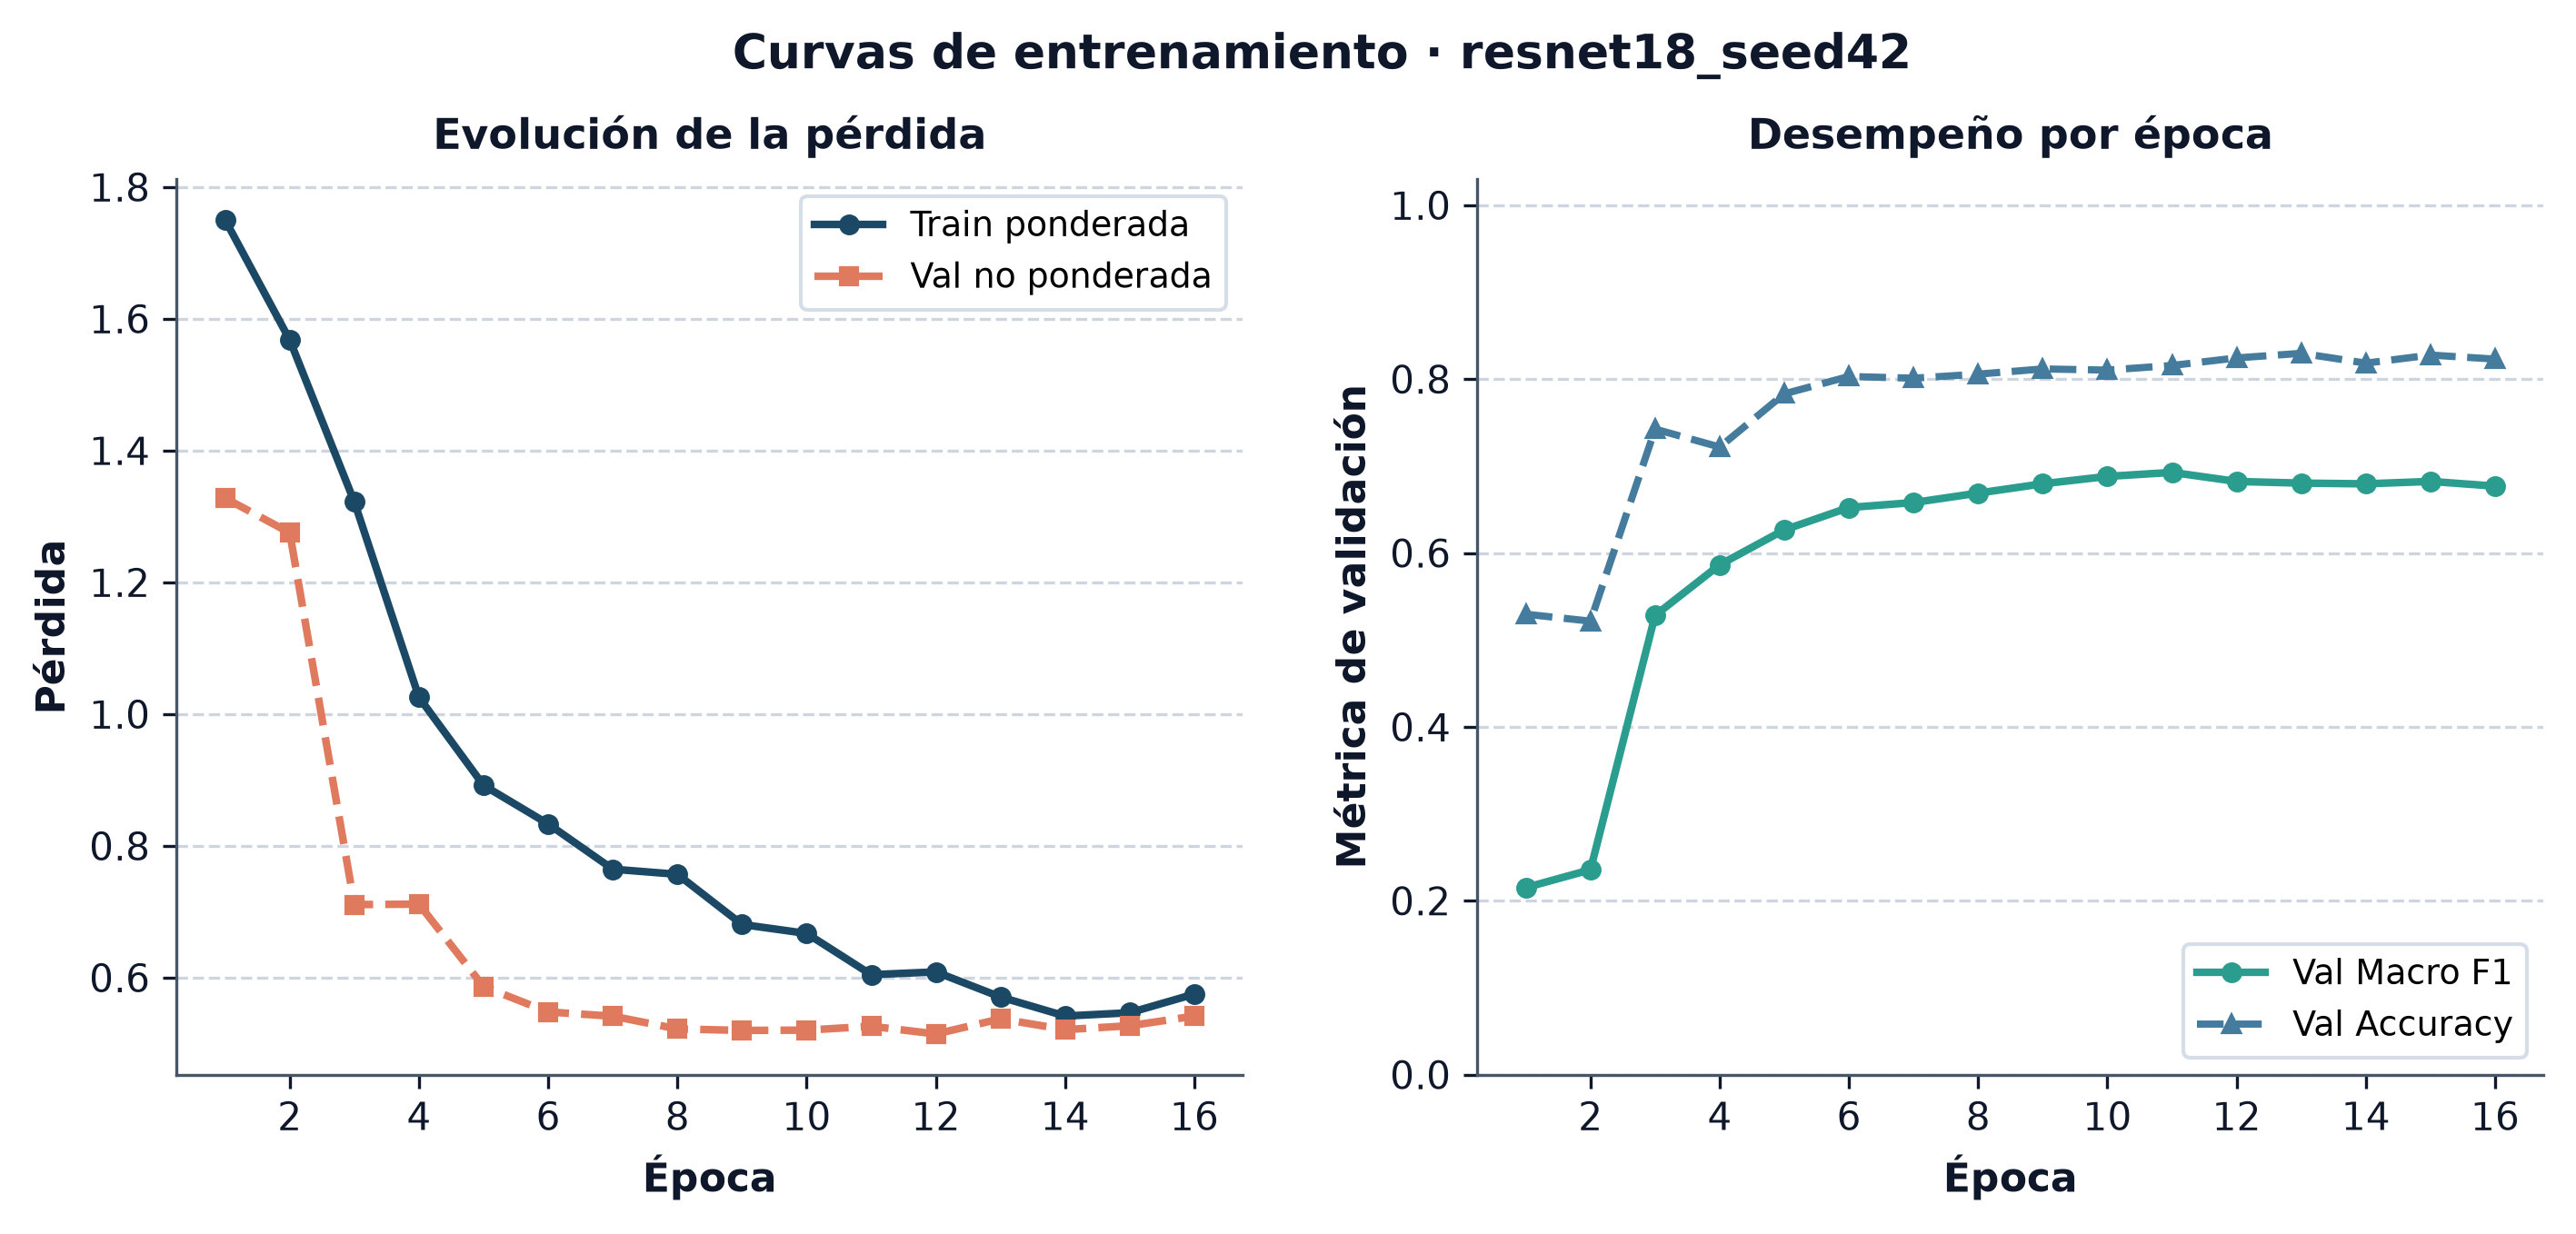
\includegraphics[width=0.92\textwidth]{curvas_resnet18_seed42.png}
\caption{Curvas reales de pérdida y métricas en validación por época para ResNet-18 (16 épocas, parada temprana; \texttt{seed=42}, \texttt{history.csv}).}
\label{fig:curvas_resnet}
\end{figure}

\begin{figure}[htbp]
\centering
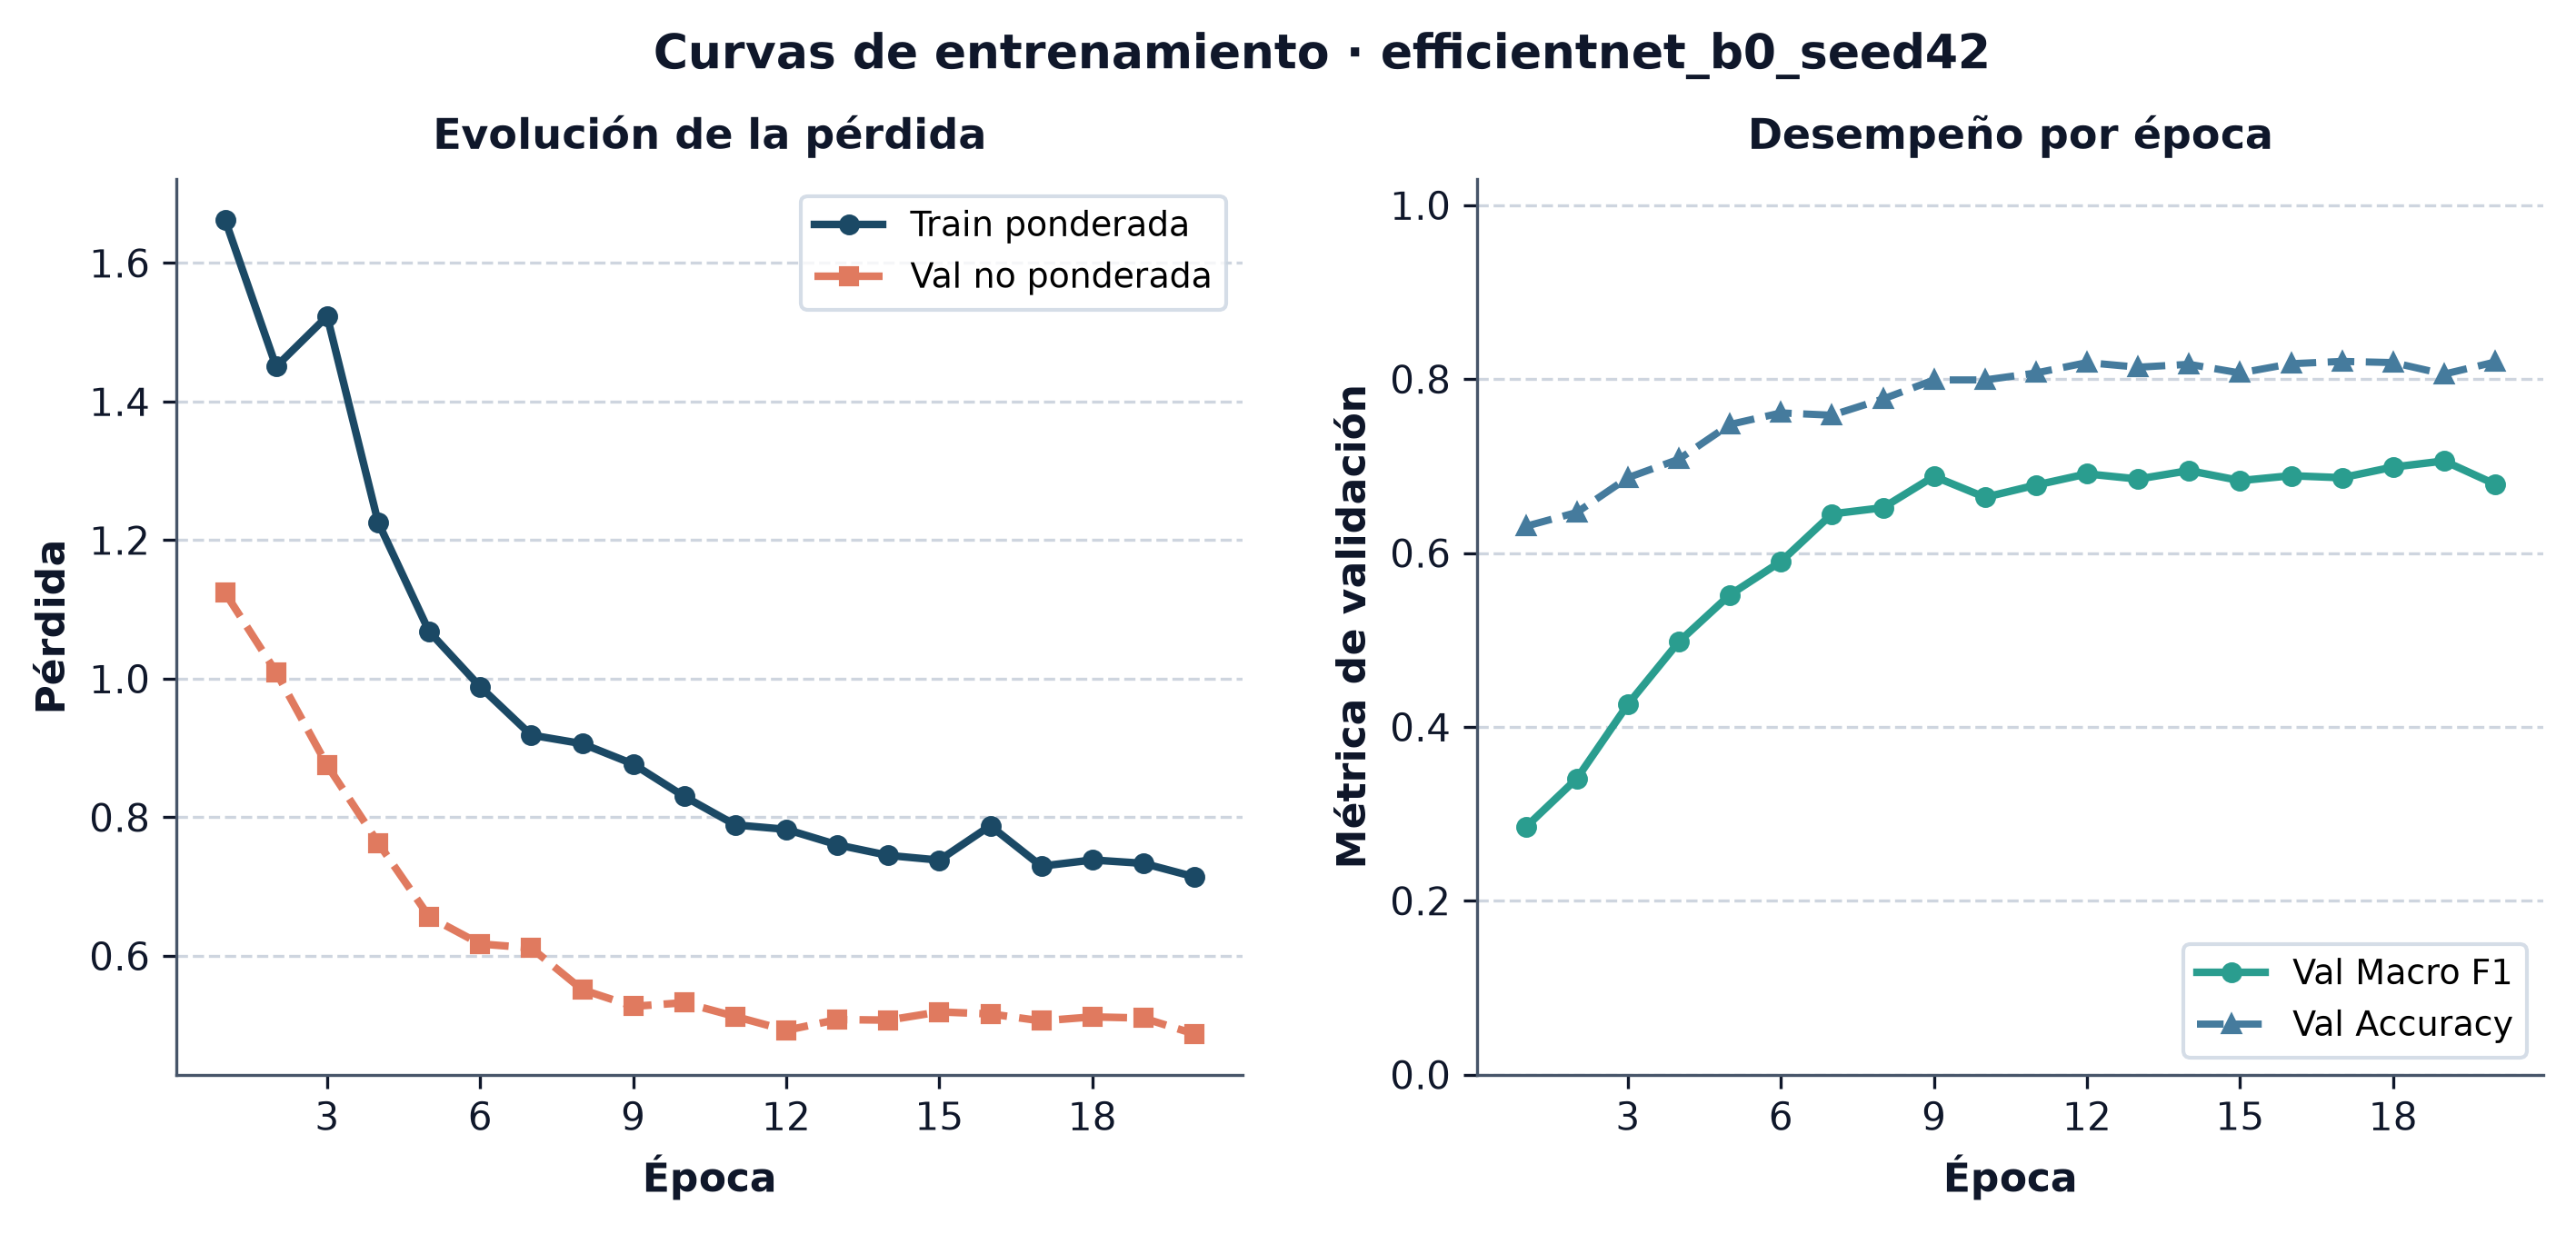
\includegraphics[width=0.92\textwidth]{curvas_efficientnet_b0_seed42.png}
\caption{Curvas reales de pérdida y métricas en validación por época para EfficientNet-B0 (20 épocas completas; \texttt{seed=42}, \texttt{history.csv}).}
\label{fig:curvas_effnet}
\end{figure}

\begin{figure}[htbp]
\centering
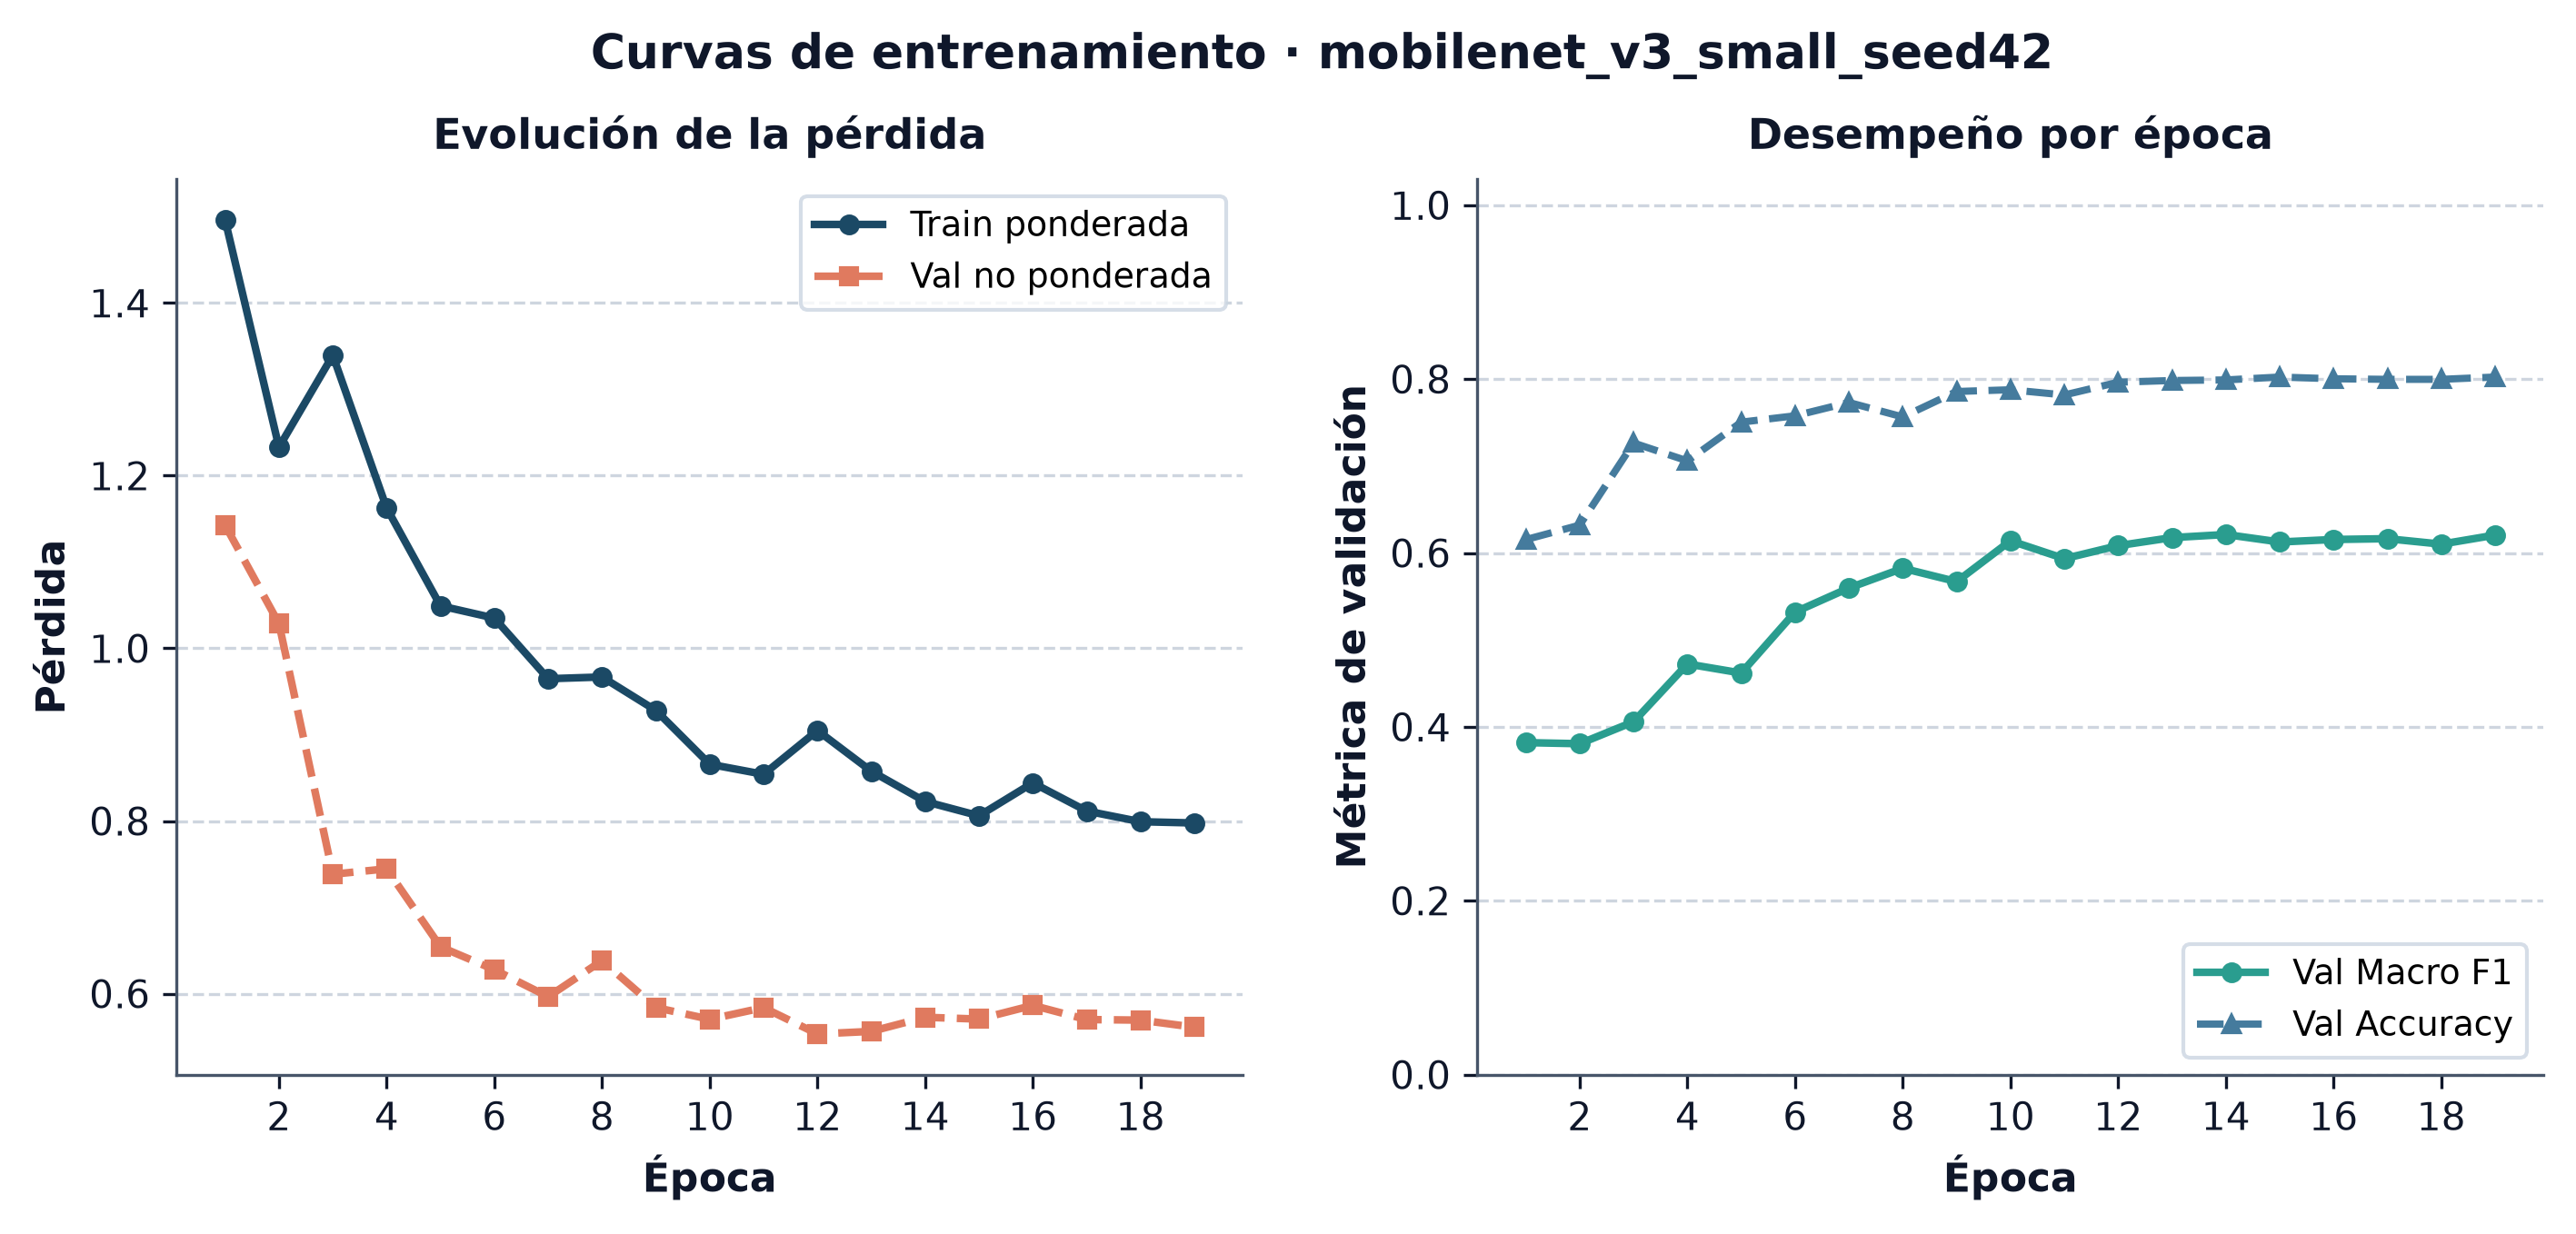
\includegraphics[width=0.92\textwidth]{curvas_mobilenet_v3_small_seed42.png}
\caption{Curvas reales de pérdida y métricas en validación por época para MobileNetV3-Small (19 épocas, parada temprana; \texttt{seed=42}, \texttt{history.csv}).}
\label{fig:curvas_mobilenet}
\end{figure}

\FloatBarrier
\subsection{Comparación global y eficiencia de los tres algoritmos}
Tras congelar los mejores checkpoints de validación (\texttt{best.pt}), se evaluó una única vez la partición \texttt{test} ($n=1\,503$) mediante \texttt{-{}-confirmar-test}. La Tabla~\ref{tab:res_global} y la Figura~\ref{fig:comp_metricas} consolidan la calidad predictiva en \texttt{test} limpio junto con el costo real medido sobre la GTX~1650.

\begin{table}[htbp]\centering\scriptsize
\setlength{\tabcolsep}{1.8pt}
\caption{Comparación global de desempeño en \texttt{test} limpio ($n=1\,503$) y eficiencia computacional entre los tres algoritmos.}
\label{tab:res_global}
\begin{tabularx}{\textwidth}{@{}>{\bfseries}l*{9}{>{\centering\arraybackslash}X}@{}}
\toprule
\textbf{Arquitectura} & \makecell{\textbf{Acc.}} & \makecell{\textbf{Macro}\\\textbf{Prec.}} & \makecell{\textbf{Macro}\\\textbf{F1}} & \makecell{\textbf{Bal.}\\\textbf{Acc.}} & \makecell{\textbf{Rec.}\\\textbf{\texttt{mel}}} & \makecell{\textbf{AUC}\\\textbf{OVR}} & \makecell{\textbf{s /}\\\textbf{época}} & \makecell{\textbf{Lat. med.}\\\textbf{(P95, ms)}} & \makecell{\textbf{VRAM}\\\textbf{(MiB)}} \\ \midrule
ResNet-18 & \textbf{0.8031} & 0.6591 & \textbf{0.6786} & \textbf{0.7174} & 0.6012 & \textbf{0.9596} & \textbf{127.5} & \makecell{\textbf{7.22}\\{\tiny (8.09)}} & 434.2 \\
EfficientNet-B0 & 0.8004 & \textbf{0.6741} & 0.6778 & 0.7025 & \textbf{0.6607} & 0.9587 & 188.6 & \makecell{24.60\\{\tiny (25.97)}} & 805.7 \\
MobileNetV3-Small & 0.7625 & 0.6474 & 0.5700 & 0.5604 & 0.4167 & 0.9407 & 156.3 & \makecell{22.40\\{\tiny (23.97)}} & \textbf{211.8} \\
\bottomrule
\end{tabularx}
\par\smallskip{\scriptsize\raggedright Nota: la latencia corresponde exclusivamente a \texttt{forward()} en GPU con \texttt{batch=1} (sin E/S ni preprocesamiento). Entre las corridas repetidas del mismo modelo en la GTX~1650 se observó dispersión operativa de $6.86$--$9.46$~ms (ResNet-18), $22.49$--$34.82$~ms (EfficientNet-B0) y $15.26$--$22.40$~ms (MobileNetV3-Small).\par}
\end{table}

\begin{figure}[htbp]
\centering
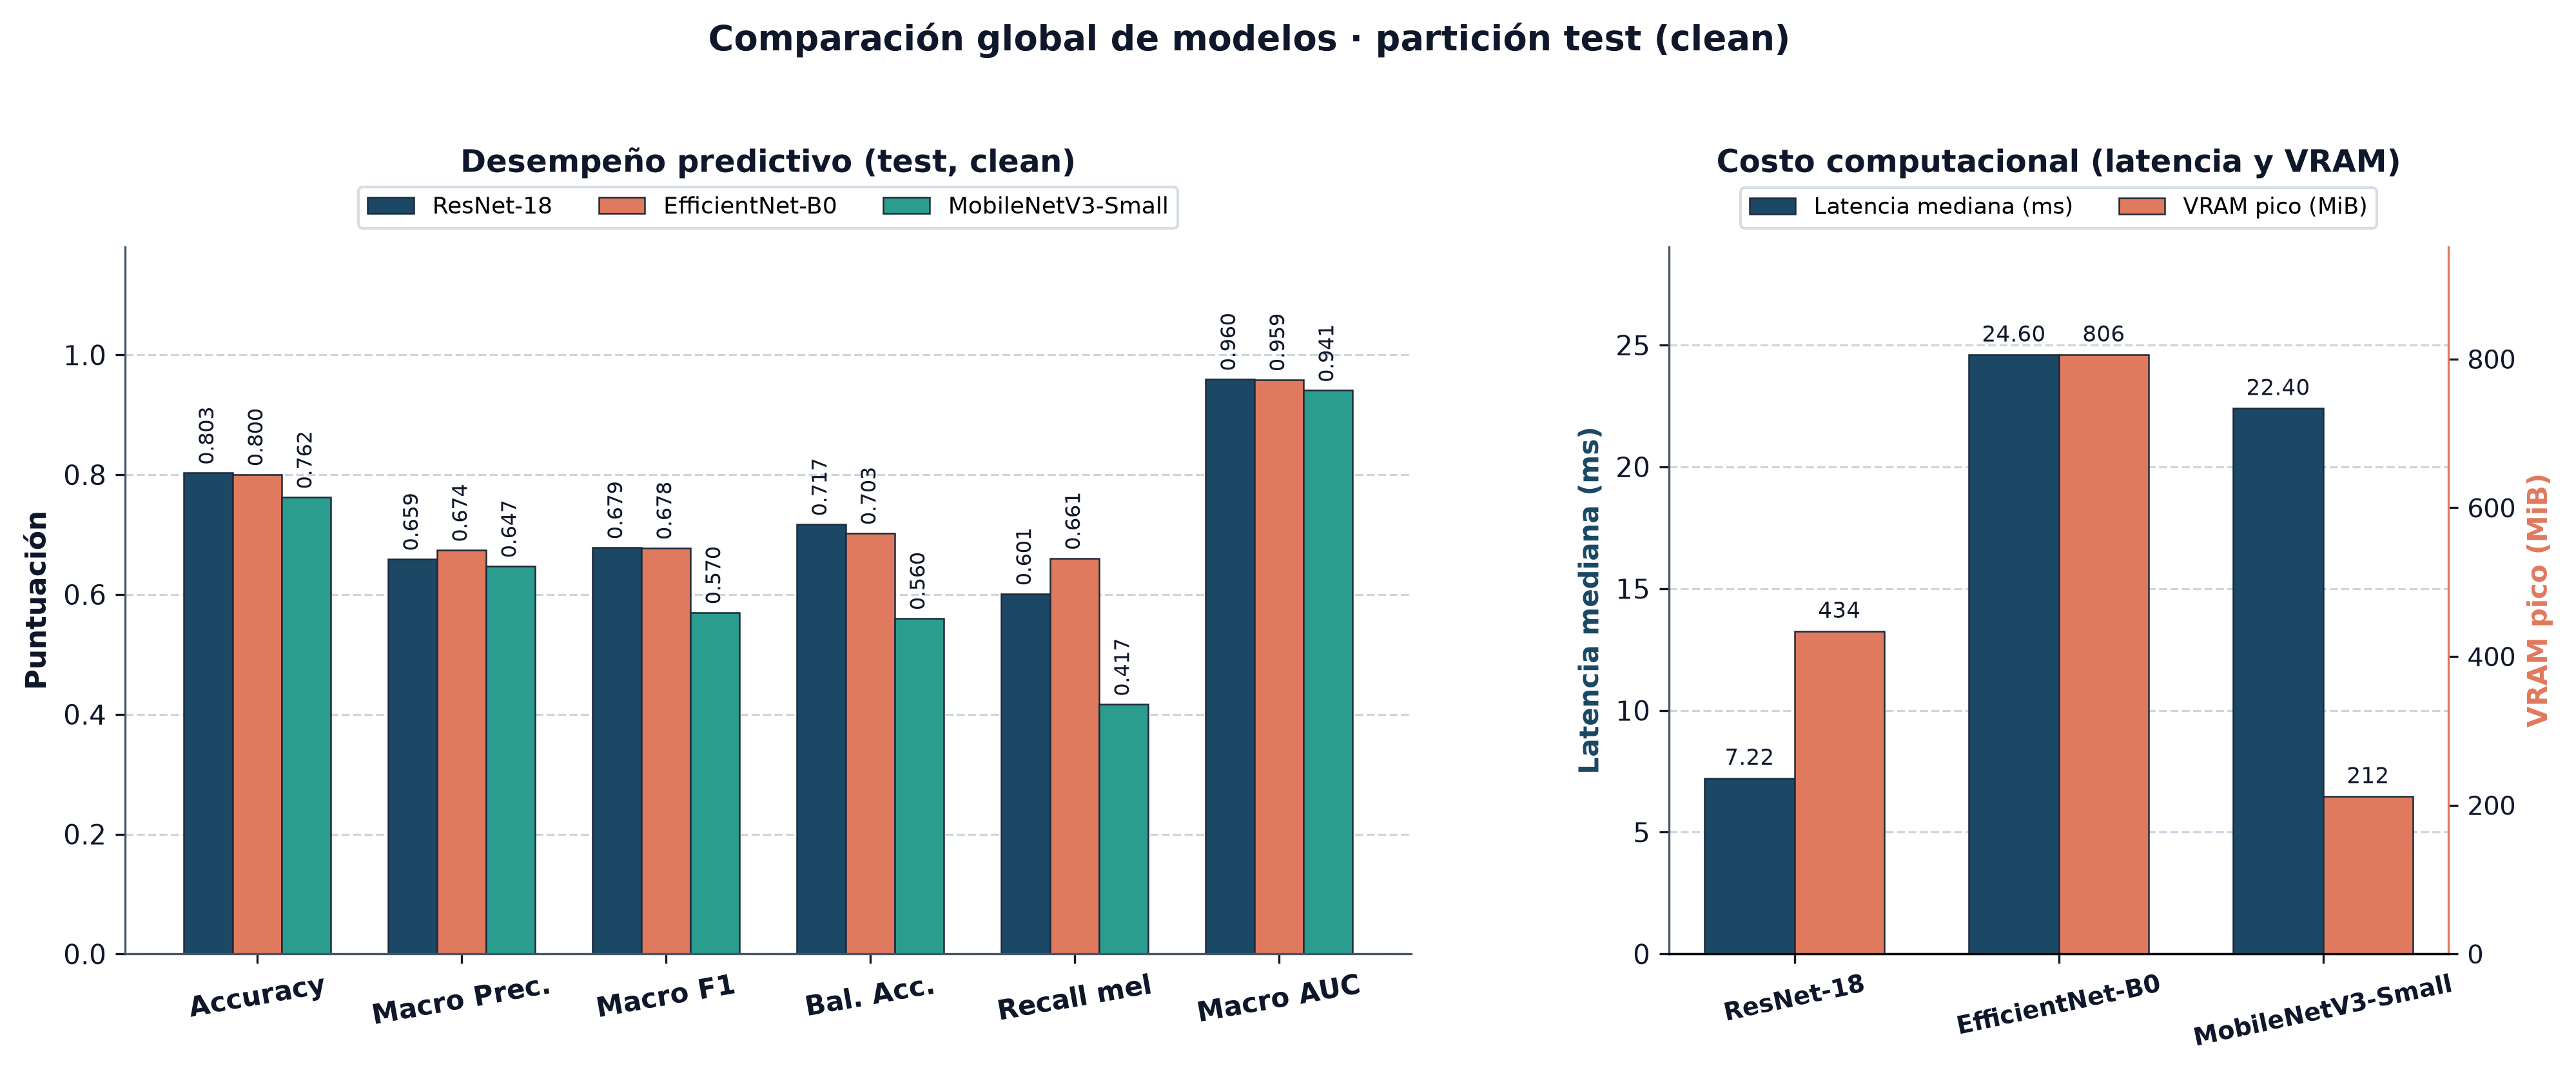
\includegraphics[width=0.96\textwidth]{comparacion_metricas.png}
\caption{Comparación visual del desempeño predictivo en \texttt{test} limpio (izquierda) y del costo computacional en GTX~1650 (derecha).}
\label{fig:comp_metricas}
\end{figure}

Los resultados globales muestran dos hallazgos relevantes. En primer lugar, bajo este protocolo común y hardware, \textbf{ResNet-18} ofrece el mejor compromiso observado desempeño--latencia (Macro~F1 = 0.6786, Macro~Prec.\ = 0.6591, \textit{Balanced Accuracy} = 0.7174, $\mathrm{AUC}_{\mathrm{OVR}}$ = 0.9596, \texttt{forward()} = 7.22~ms), frente a \textbf{EfficientNet-B0} (Macro~F1 = 0.6778, Macro~Prec.\ = 0.6741, mayor sensibilidad limpia en melanoma con 0.6607 vs.\ 0.6012). Sin embargo, la diferencia puntual de $0.00084$ en Macro~F1 entre ambas arquitecturas \textbf{no demuestra superioridad estadística ni equivalencia}: un análisis complementario por \textit{bootstrap} pareado sobre los $1\,118$ grupos independientes (\texttt{group\_id}) de \texttt{test} arroja un intervalo de confianza al 95\% de $[-0.0429, +0.0464]$. En cambio, \textbf{MobileNetV3-Small} pierde más de 10.8 puntos porcentuales en Macro~F1 (0.5700) y 15.7 puntos en \textit{Balanced Accuracy} (0.5604), aunque su \textit{Accuracy} aparente (0.7625) luzca elevada por el peso de la clase mayoritaria \texttt{nv}.

En segundo lugar, en eficiencia real sobre GPU GTX~1650 en FP32, \textbf{ResNet-18} entrena en 127.5~s/época y registra una latencia mediana de \texttt{forward()} (\texttt{batch=1}, excluyendo lectura en disco y preprocesamiento) de \textbf{7.22~ms} (P95 = 8.09~ms; rango entre corridas repetidas: $6.86$--$9.46$~ms), frente a $22.40$~ms en MobileNetV3-Small (rango $15.26$--$22.40$~ms) y $24.60$~ms en EfficientNet-B0 (rango $22.49$--$34.82$~ms). Aunque MobileNetV3-Small minimiza el pico de VRAM (211.8~MiB frente a 434.2~MiB en ResNet-18 y 805.7~MiB en EfficientNet-B0), una hipótesis interpretativa plausible (no verificada mediante perfilado de núcleos ni estudios de ablación) es que la secuencia profunda de capas separables, bloques SE y activaciones \textit{h-swish} genere mayor sobrecarga de lanzamiento de núcleos y fragmentación de accesos en CUDA que las convoluciones residuales estándar $3\times 3$ de ResNet-18 en \texttt{batch=1}.

\FloatBarrier
\subsection{Comparación detallada por categoría diagnóstica}
Debido al desbalance de $58.3:1$, la Tabla~\ref{tab:res_clases} desglosa \textit{Precision}, \textit{Recall}, F1 y $\mathrm{AUC}_{\mathrm{OVR}}$ sobre las siete categorías diagnósticas de \texttt{test} ($n=1\,503$), complementada con las matrices de confusión (Figuras~\ref{fig:conf_resnet}--\ref{fig:conf_mobilenet}) y las curvas ROC OVR comparativas e individuales (Figuras~\ref{fig:roc_comp} y~\ref{fig:roc_resnet}--\ref{fig:roc_mobilenet}).

\begin{table}[htbp]\centering\scriptsize
\setlength{\tabcolsep}{1.3pt}
\caption{Desglose comparativo de Precision (P), Recall (R), F1 y AUC OVR por clase en el conjunto fijo \texttt{test} ($n=1\,503$).}
\label{tab:res_clases}
\begin{tabular*}{\textwidth}{@{\extracolsep{\fill}}>{\ttfamily}lrr*{12}{r}@{}}
\toprule
\textrm{\textbf{Clase}} & \makecell[r]{\textbf{Sop.}\\\textbf{\texttt{test}}} & \makecell[r]{\textbf{$w_c$}\\\textbf{\texttt{train}}} & \multicolumn{4}{c}{\textbf{ResNet-18}} & \multicolumn{4}{c}{\textbf{EfficientNet-B0}} & \multicolumn{4}{c}{\textbf{MobileNetV3-Small}} \\
\cmidrule(lr){4-7}\cmidrule(lr){8-11}\cmidrule(lr){12-15}
 & & & \textbf{P} & \textbf{R} & \textbf{F1} & \textbf{AUC} & \textbf{P} & \textbf{R} & \textbf{F1} & \textbf{AUC} & \textbf{P} & \textbf{R} & \textbf{F1} & \textbf{AUC} \\ \midrule
akiec & 49 & 4.3916 & 0.6889 & \textbf{0.6327} & 0.6596 & 0.9791 & \textbf{0.8571} & 0.6122 & \textbf{0.7143} & \textbf{0.9878} & 0.7273 & 0.1633 & 0.2667 & 0.9743 \\
bcc & 78 & 2.7891 & \textbf{0.7812} & 0.6410 & \textbf{0.7042} & \textbf{0.9798} & 0.7500 & 0.6154 & 0.6761 & 0.9743 & 0.6118 & \textbf{0.6667} & 0.6380 & 0.9720 \\
bkl & 165 & 1.3021 & 0.5967 & 0.6545 & 0.6243 & \textbf{0.9320} & \textbf{0.6054} & \textbf{0.6788} & \textbf{0.6400} & 0.9261 & 0.4589 & 0.6424 & 0.5354 & 0.8881 \\
df & 17 & 12.5161 & 0.4000 & \textbf{0.7059} & \textbf{0.5106} & \textbf{0.9882} & 0.3750 & 0.5294 & 0.4390 & 0.9708 & \textbf{0.5556} & 0.2941 & 0.3846 & 0.9692 \\
mel & 168 & 1.2853 & \textbf{0.5233} & 0.6012 & 0.5596 & 0.8947 & 0.4868 & \textbf{0.6607} & \textbf{0.5606} & \textbf{0.9113} & 0.4698 & 0.4167 & 0.4416 & 0.8594 \\
nv & 1\,005 & 0.2133 & 0.9200 & 0.8816 & \textbf{0.9004} & 0.9458 & \textbf{0.9297} & 0.8687 & 0.8981 & \textbf{0.9488} & 0.8906 & \textbf{0.8826} & 0.8866 & 0.9281 \\
vasc & 21 & 10.0129 & 0.7037 & 0.9048 & 0.7917 & \textbf{0.9976} & 0.7143 & \textbf{0.9524} & 0.8163 & 0.9921 & \textbf{0.8182} & 0.8571 & \textbf{0.8372} & 0.9938 \\ \midrule
\textrm{\textbf{Macro}} & \textbf{1\,503} & --- & 0.6591 & \textbf{0.7174} & \textbf{0.6786} & \textbf{0.9596} & \textbf{0.6741} & 0.7025 & 0.6778 & 0.9587 & 0.6474 & 0.5604 & 0.5700 & 0.9407 \\
\bottomrule
\end{tabular*}
\end{table}

\begin{figure}[htbp]
\centering
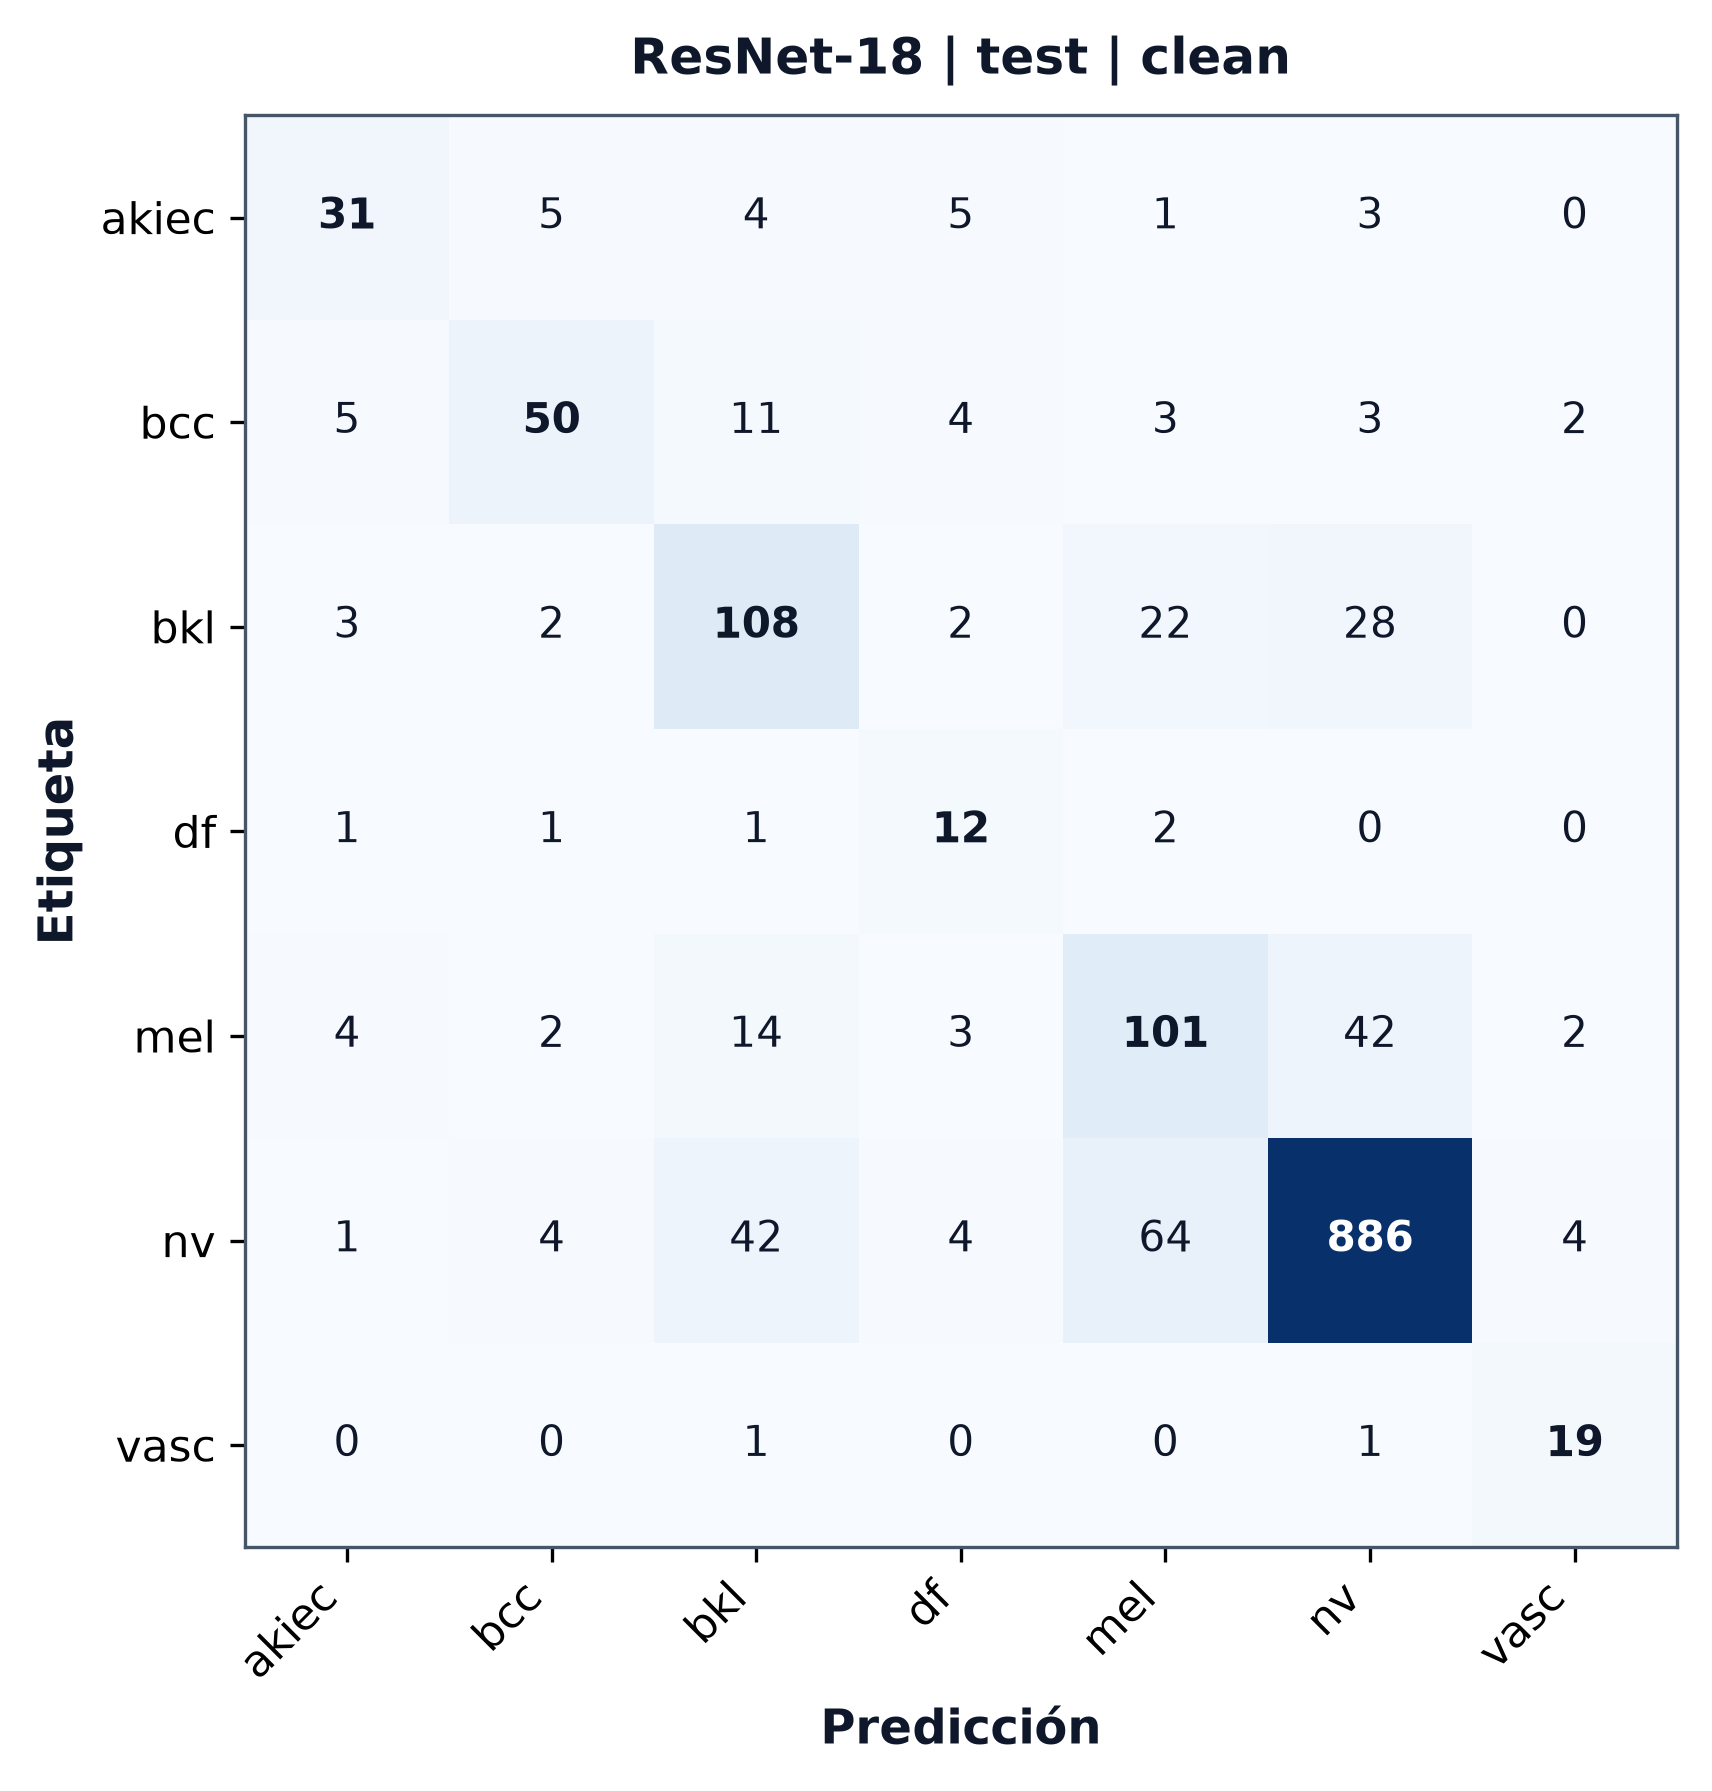
\includegraphics[width=0.68\textwidth]{confusion_resnet18_42_test_clean.png}
\caption{Matriz de confusión $7\times 7$ de ResNet-18 en \texttt{test} limpio ($n=1\,503$, \texttt{seed=42}).}
\label{fig:conf_resnet}
\end{figure}

\begin{figure}[htbp]
\centering
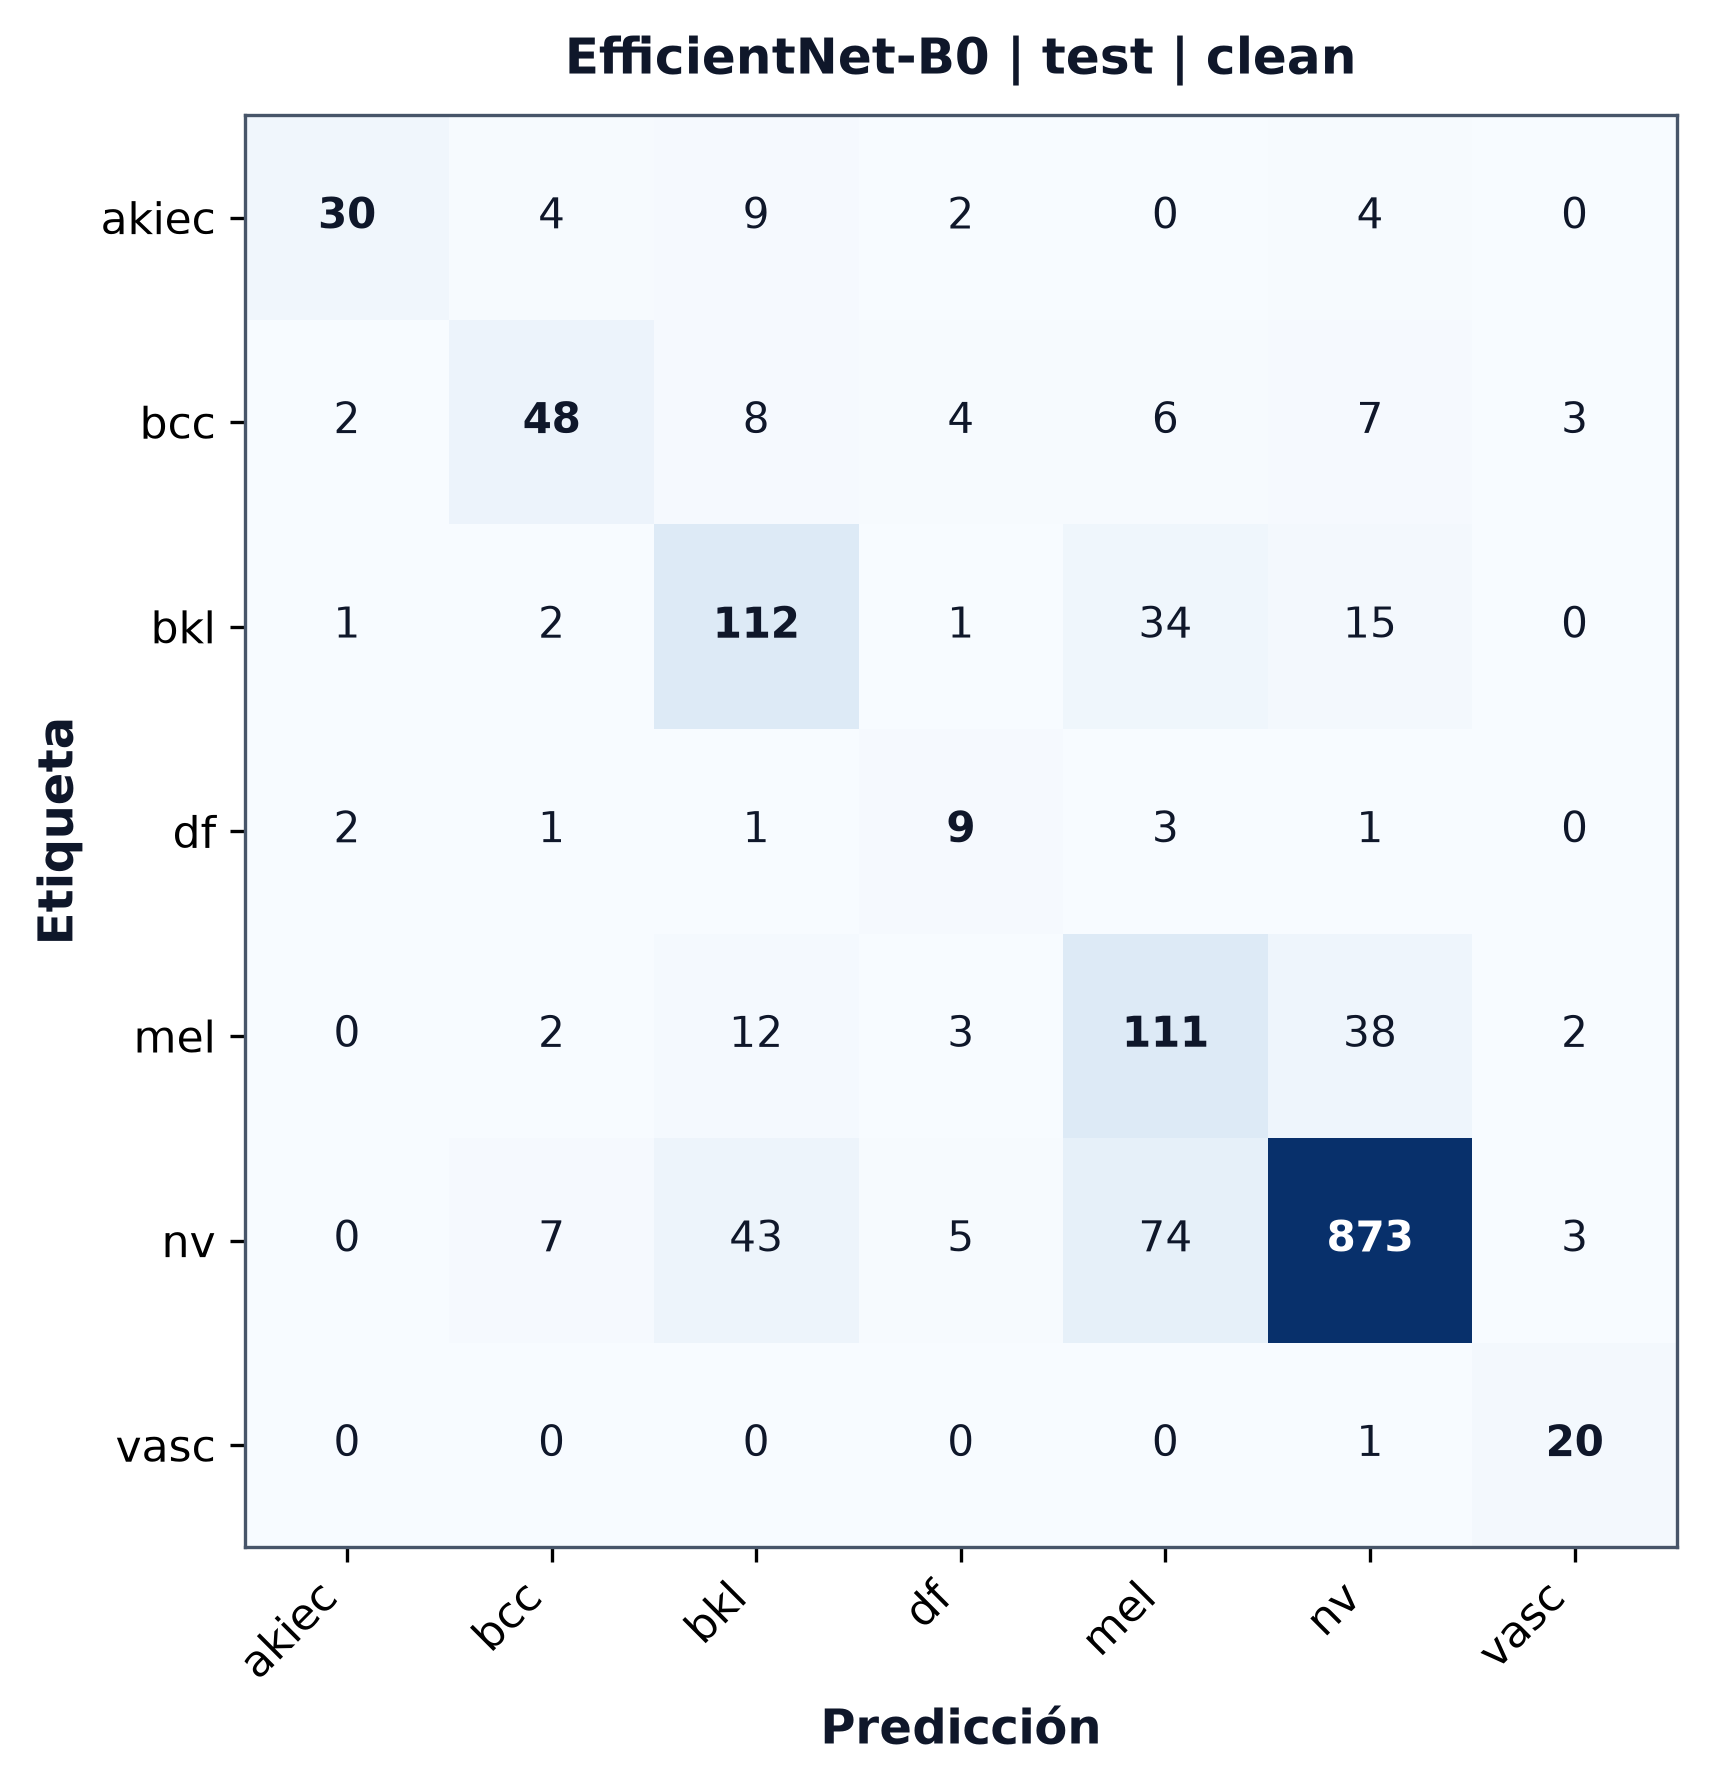
\includegraphics[width=0.68\textwidth]{confusion_efficientnet_b0_42_test_clean.png}
\caption{Matriz de confusión $7\times 7$ de EfficientNet-B0 en \texttt{test} limpio ($n=1\,503$, \texttt{seed=42}).}
\label{fig:conf_effnet}
\end{figure}

\begin{figure}[htbp]
\centering
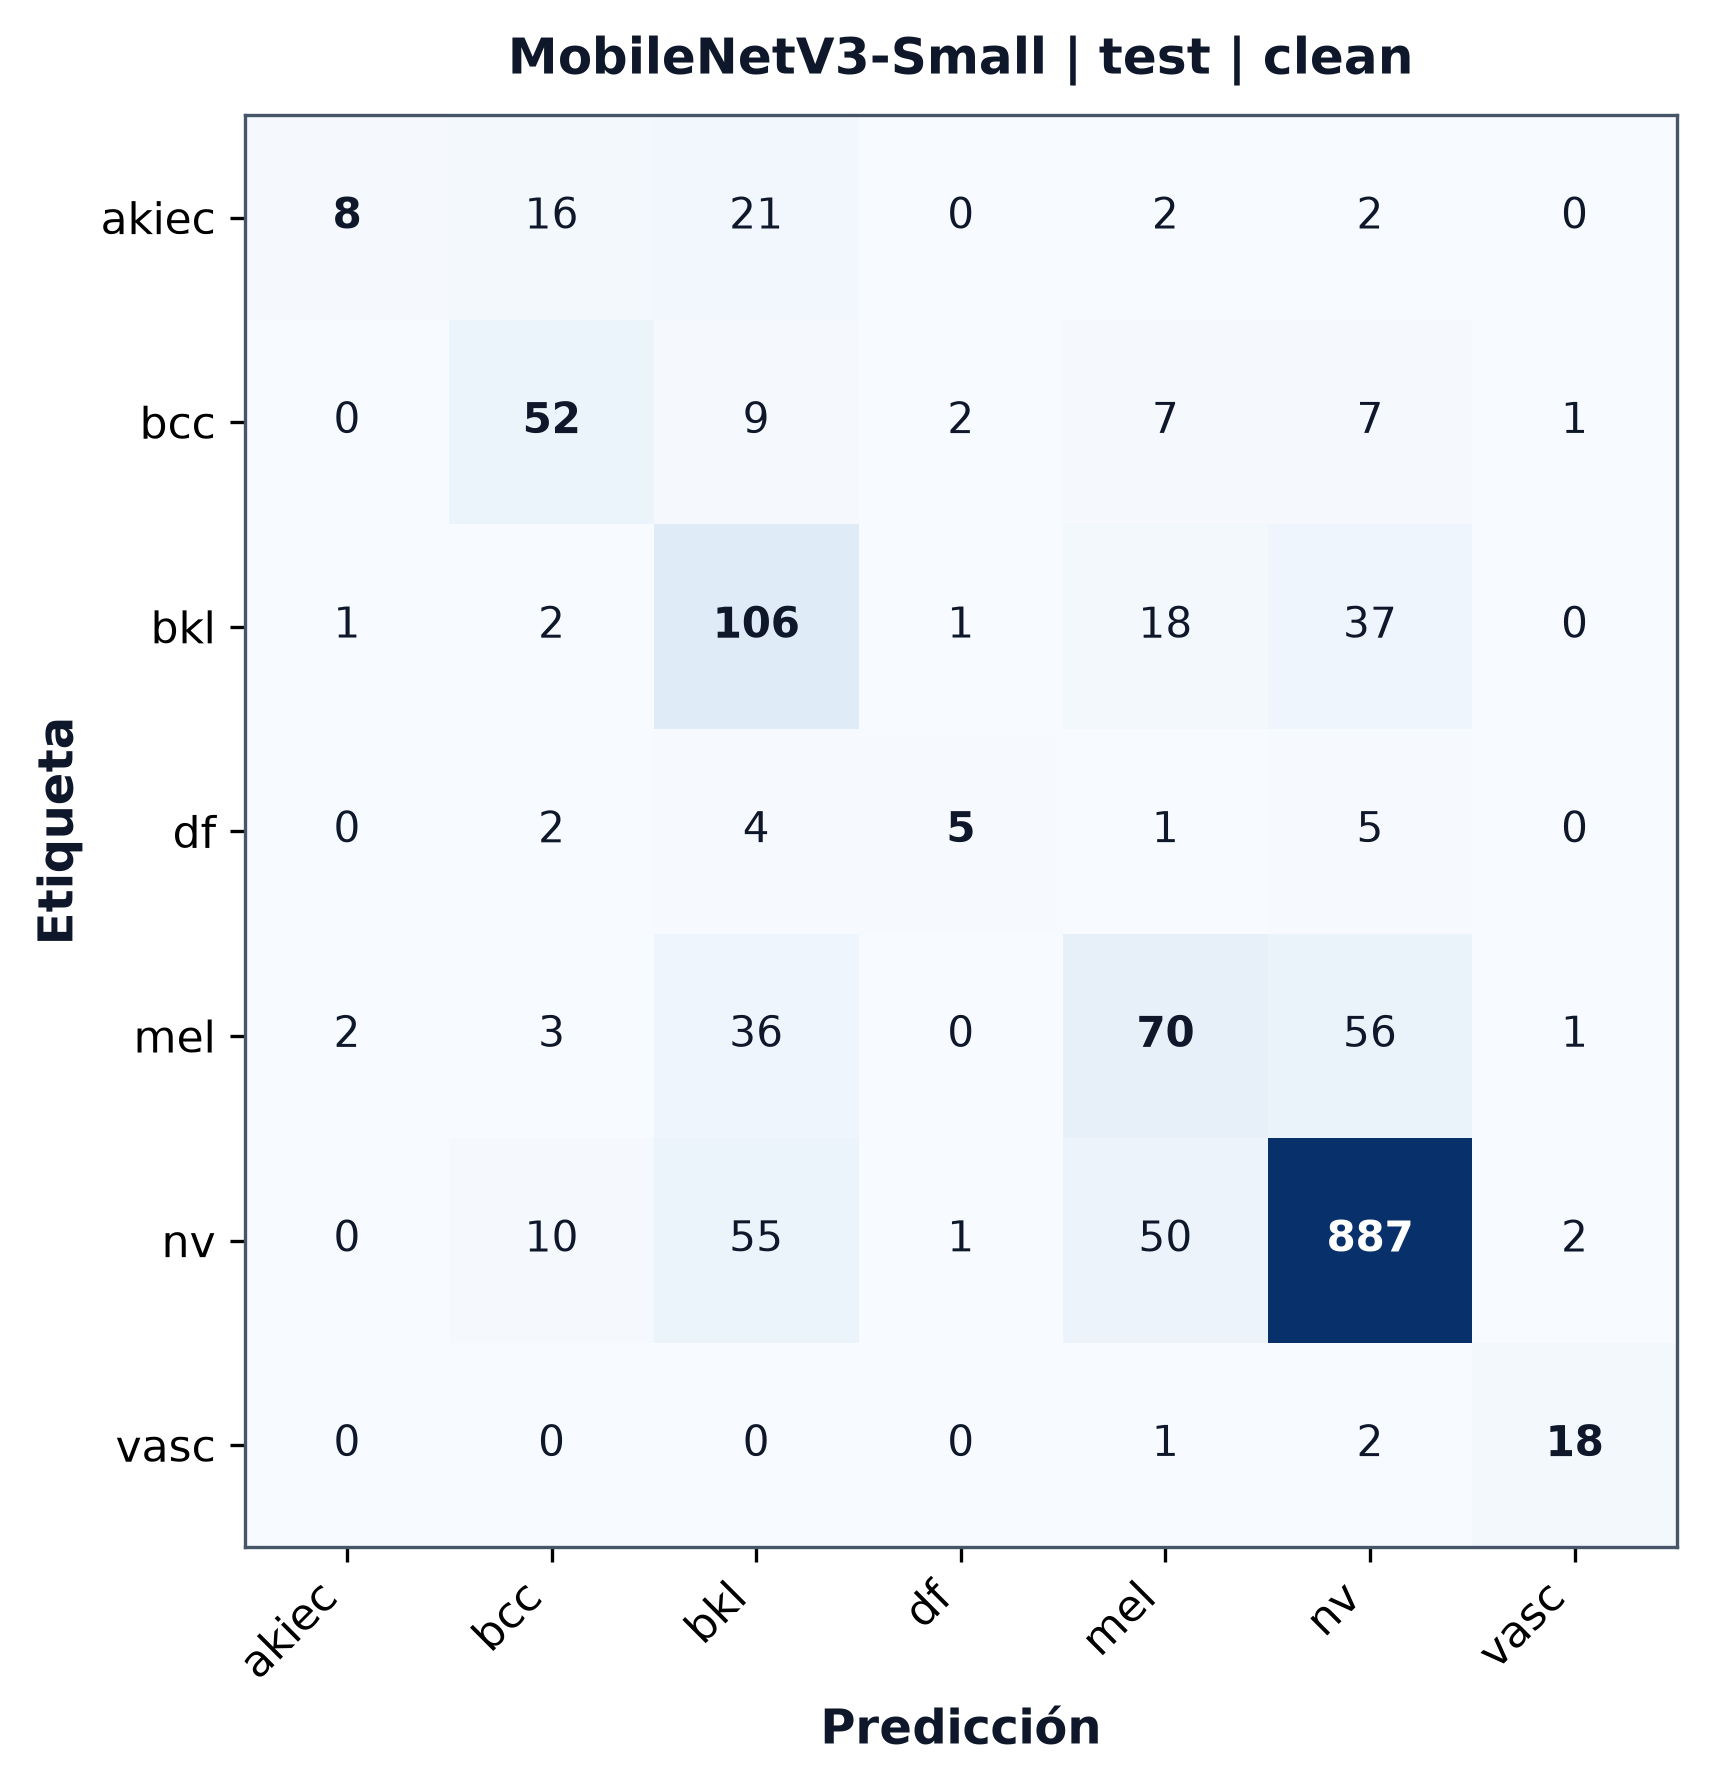
\includegraphics[width=0.68\textwidth]{confusion_mobilenet_v3_small_42_test_clean.png}
\caption{Matriz de confusión $7\times 7$ de MobileNetV3-Small en \texttt{test} limpio ($n=1\,503$, \texttt{seed=42}).}
\label{fig:conf_mobilenet}
\end{figure}
\FloatBarrier

El análisis por categoría revela dónde se origina la brecha entre modelos:
\begin{itemize}[leftmargin=1.4em,itemsep=3pt]
\item \textbf{Melanoma (\texttt{mel}, $n=168$):} es la categoría más crítica y difícil de separar. EfficientNet-B0 alcanza la mayor sensibilidad (0.6607; 111/168 aciertos) y F1 (0.5606) con \textit{Precision} de 0.4868, mientras ResNet-18 logra mayor \textit{Precision} (0.5233), \textit{Recall} de 0.6012 (101/168 aciertos; 92 falsos positivos, 67 falsos negativos) y F1 muy cercano (0.5596) gracias a menor tasa de confusión desde \texttt{nv} (64 casos frente a 74 en EfficientNet-B0) y \texttt{bkl} (22 frente a 34). MobileNetV3-Small cae a 0.4167 de sensibilidad (solo 70/168, \textit{Precision} = 0.4698), confundiendo 56 melanomas con \texttt{nv} y 36 con \texttt{bkl}.
\item \textbf{Clases minoritarias (\texttt{akiec}, \texttt{df}, \texttt{vasc}):} en \texttt{vasc} ($n=21$), las tres redes logran alta separabilidad (F1 entre 0.7917 y 0.8372; 18--20 aciertos). En cambio, en \texttt{akiec} ($n=49$) y \texttt{df} ($n=17$) MobileNetV3-Small colapsa en cobertura: aunque mantiene \textit{Precision} moderada (0.7273 en \texttt{akiec}, 0.5556 en \texttt{df}), solo acierta 8/49 en \texttt{akiec} (\textit{Recall} = 0.1633, F1 = 0.2667, derivando 21 casos a \texttt{bkl} y 16 a \texttt{bcc}) y 5/17 en \texttt{df} (\textit{Recall} = 0.2941, F1 = 0.3846). ResNet-18 lidera en \texttt{df} (F1 = 0.5106, \textit{Recall} = 0.7059; 12/17) y \texttt{bcc} (F1 = 0.7042, \textit{Precision} = 0.7812), mientras EfficientNet-B0 lidera en \texttt{akiec} (P = 0.8571, F1 = 0.7143) y \texttt{bkl} (P = 0.6054, F1 = 0.6400).
\item \textbf{Clase mayoritaria (\texttt{nv}, $n=1\,005$):} las tres arquitecturas muestran comportamiento homogéneo (\textit{Precision} entre 0.8906 y 0.9297; F1 entre 0.8866 y 0.9004), confirmando que el uso de pesos $w_c$ evita el colapso hacia \texttt{nv}, aunque persiste una confusión bidireccional moderada en la frontera pigmentada \texttt{nv}--\texttt{mel}--\texttt{bkl}.
\end{itemize}

\begin{figure}[htbp]
\centering
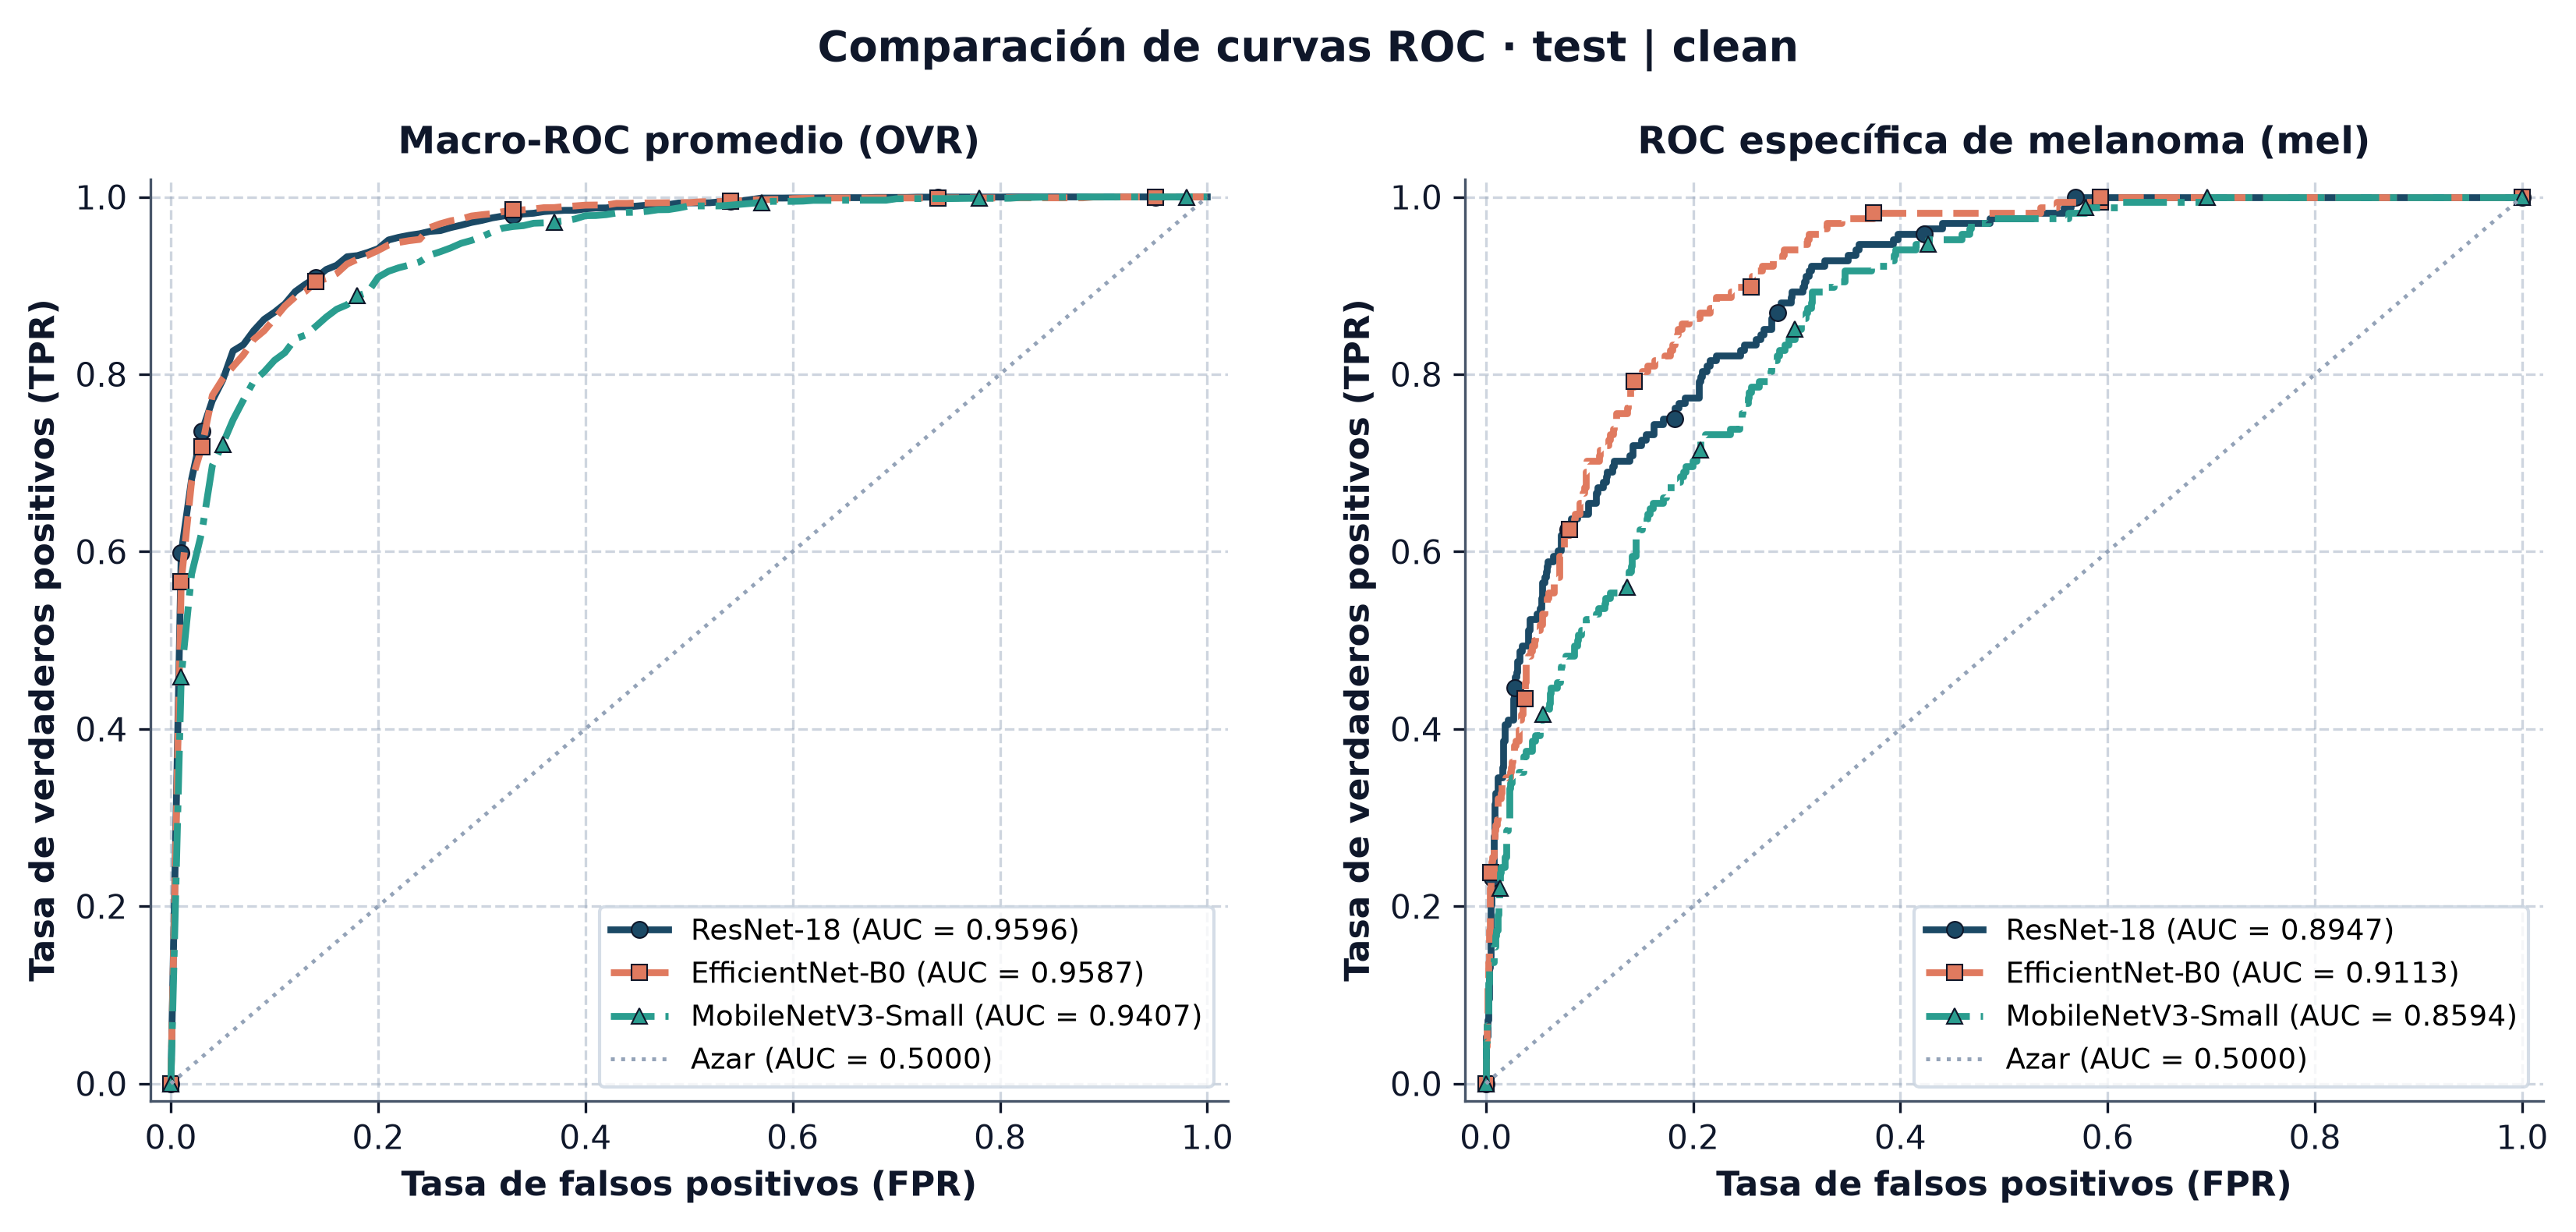
\includegraphics[width=0.96\textwidth]{roc_comparativa_test_clean.png}
\caption{Comparación de curvas ROC OVR macro-promedio (izquierda) y específica para melanoma (derecha) en \texttt{test} limpio.}
\label{fig:roc_comp}
\end{figure}

\begin{figure}[htbp]
\centering
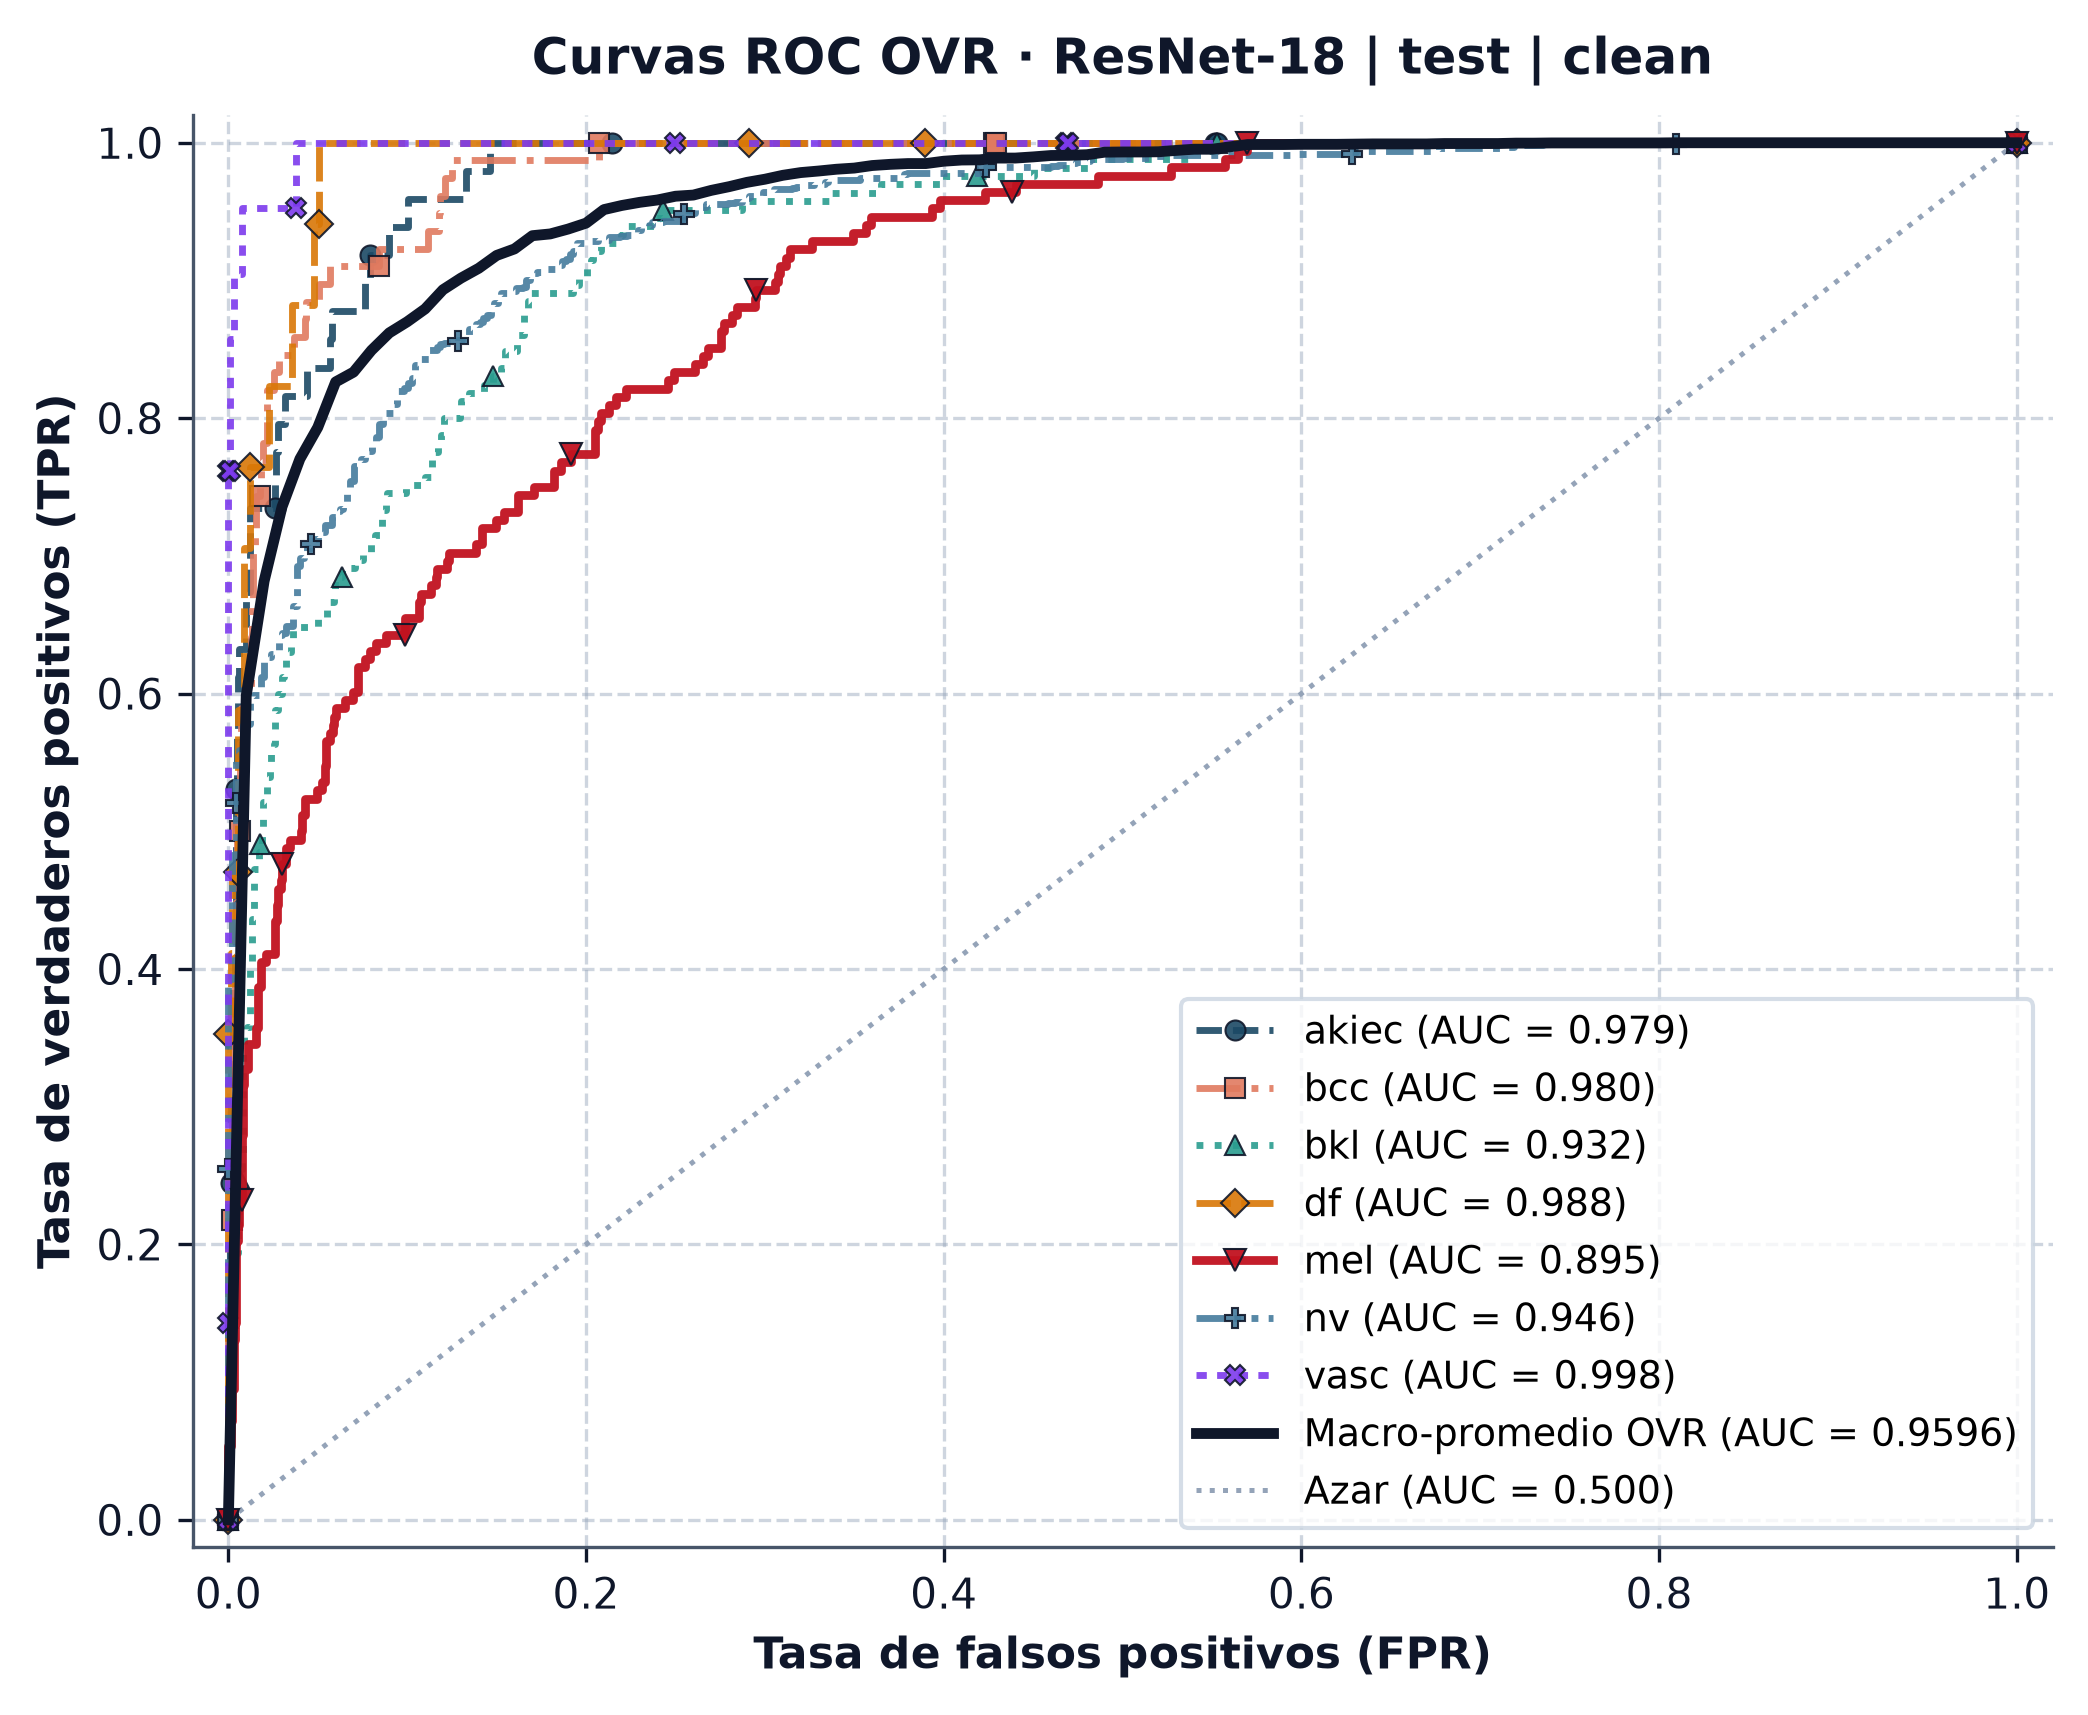
\includegraphics[width=0.78\textwidth]{roc_resnet18_42_test_clean.png}
\caption{Curvas ROC uno contra el resto (OVR) por clase en \texttt{test} limpio para ResNet-18 (\texttt{seed=42}).}
\label{fig:roc_resnet}
\end{figure}

\begin{figure}[htbp]
\centering
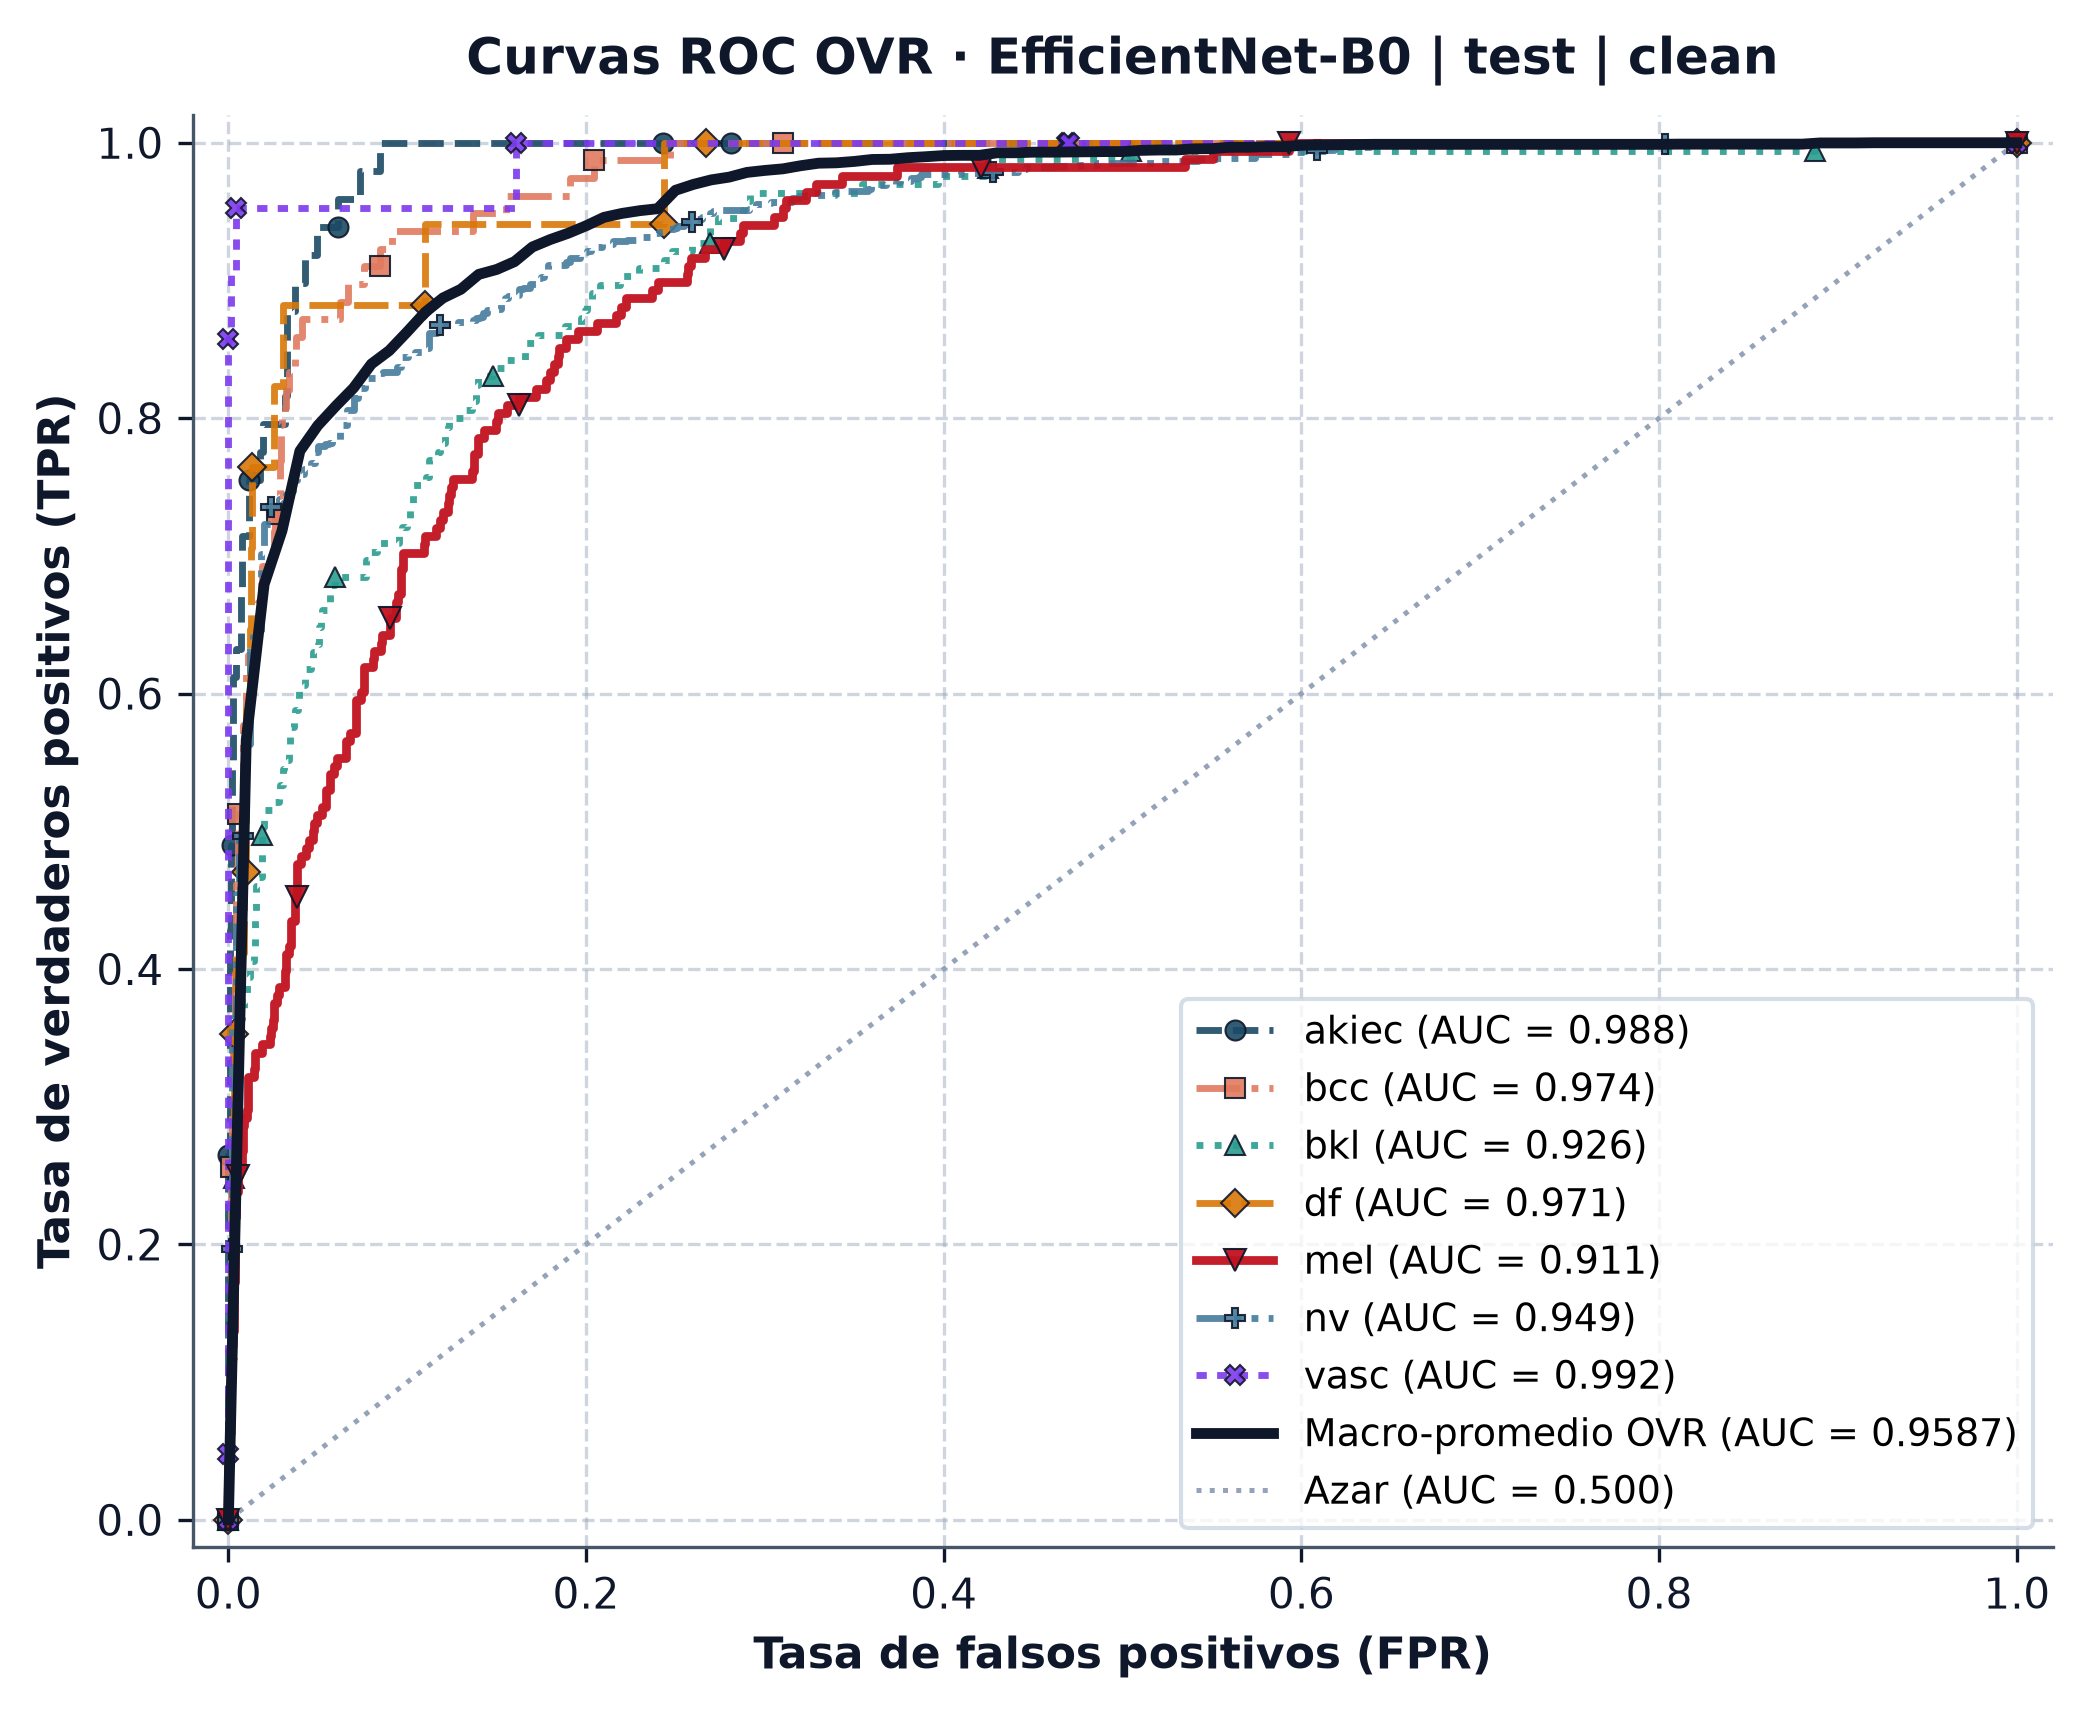
\includegraphics[width=0.78\textwidth]{roc_efficientnet_b0_42_test_clean.png}
\caption{Curvas ROC uno contra el resto (OVR) por clase en \texttt{test} limpio para EfficientNet-B0 (\texttt{seed=42}).}
\label{fig:roc_effnet}
\end{figure}

\begin{figure}[htbp]
\centering
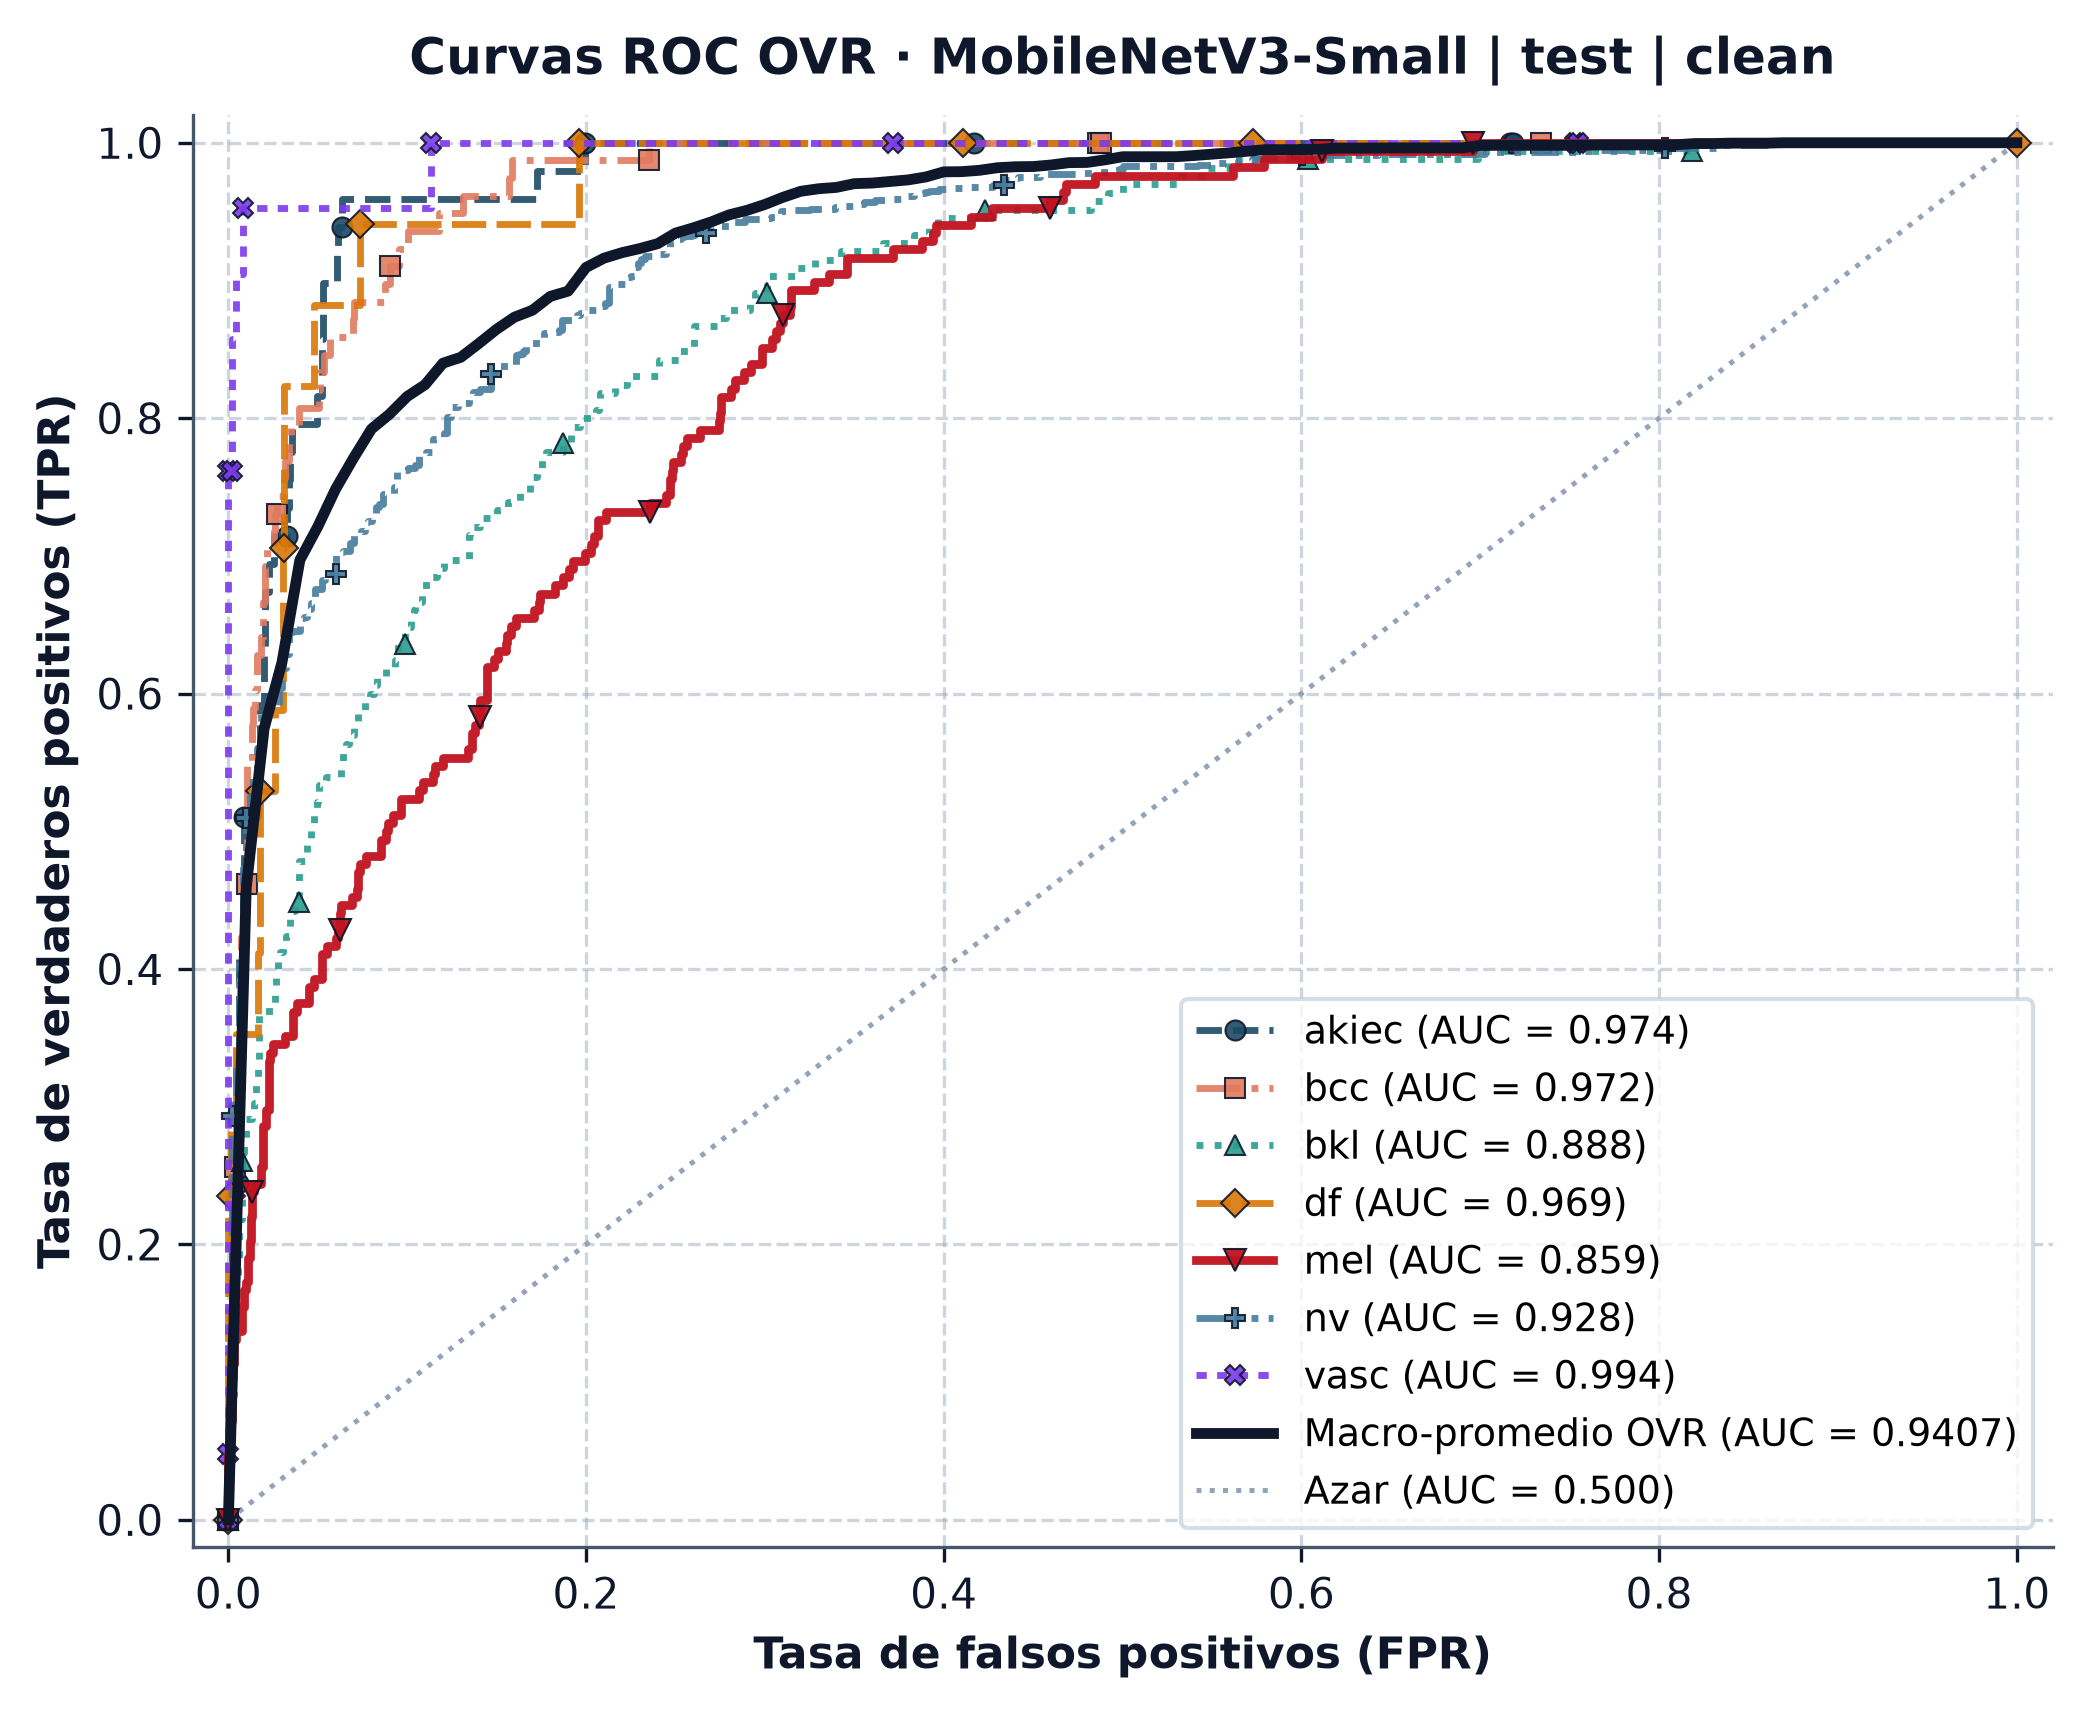
\includegraphics[width=0.78\textwidth]{roc_mobilenet_v3_small_42_test_clean.png}
\caption{Curvas ROC uno contra el resto (OVR) por clase en \texttt{test} limpio para MobileNetV3-Small (\texttt{seed=42}).}
\label{fig:roc_mobilenet}
\end{figure}
\FloatBarrier

Las curvas ROC OVR (Figuras~\ref{fig:roc_comp} y~\ref{fig:roc_resnet}--\ref{fig:roc_mobilenet}) corroboran un alto poder de ordenamiento probabilístico global ($\mathrm{AUC}_{\mathrm{OVR}}$ macro de 0.9596 en ResNet-18, 0.9587 en EfficientNet-B0 y 0.9407 en MobileNetV3-Small). En el análisis individual por clase, \texttt{mel} registra sistemáticamente el AUC más bajo de las siete categorías (0.8947 en ResNet-18, 0.9113 en EfficientNet-B0 y 0.8594 en MobileNetV3-Small), frente a valores superiores a 0.97 en \texttt{vasc}, \texttt{bcc} y \texttt{akiec}, y $\mathrm{AUC}_{\mathrm{OVR}} \ge 0.969$ en \texttt{df} (0.9692 en MobileNetV3-Small, 0.9708 en EfficientNet-B0 y 0.9882 en ResNet-18), lo cual confirma que el solapamiento morfológico de \texttt{mel} con \texttt{nv} y \texttt{bkl} constituye la principal barrera del problema.

\FloatBarrier
\subsection{Comparación de sensibilidad ante ruido, desenfoque y mitigación espacial}
La Tabla~\ref{tab:res_rob} reporta la estabilidad de Macro~F1 y las caídas máximas ($\Delta F1$ y $\Delta\mathrm{Rec.\ mel}$) frente a las cinco condiciones deterministas en \texttt{test}, mientras las Tablas~\ref{tab:res_mit} y~\ref{tab:res_mel_tradeoff} junto con la Figura~\ref{fig:comp_rob} cuantifican tanto la recuperación agregada como el intercambio entre \textit{Precision}, \textit{Recall} y falsos positivos en melanoma sobre \texttt{noise\_005}.

\begin{table}[htbp]\centering\footnotesize
\setlength{\tabcolsep}{2.5pt}
\caption{Comparación de robustez en Macro F1 bajo ruido gaussiano y desenfoque en \texttt{test} ($n=1\,503$).}
\label{tab:res_rob}
\begin{tabularx}{\textwidth}{@{}>{\bfseries}l*{7}{>{\centering\arraybackslash}X}@{}}
\toprule
\textbf{Arquitectura} & \textbf{\texttt{clean}} & \textbf{\texttt{noise\_002}} & \textbf{\texttt{noise\_005}} & \textbf{\texttt{blur\_1}} & \textbf{\texttt{blur\_2}} & \makecell{\textbf{$\Delta F1$}\\\textbf{máx.}} & \makecell{\textbf{$\Delta\mathrm{Rec.}$}\\\textbf{\texttt{mel} máx.}} \\ \midrule
ResNet-18 & \textbf{0.6786} & \textbf{0.4561} & 0.2710 & \textbf{0.5769} & \textbf{0.4895} & +0.4076 & +0.4762 \\
EfficientNet-B0 & 0.6778 & 0.2745 & 0.1201 & 0.5167 & 0.2815 & +0.5577 & +0.6607 \\
MobileNetV3-Small & 0.5700 & 0.3580 & \textbf{0.3079} & 0.5398 & 0.3949 & +0.2621 & +0.3333 \\
\bottomrule
\end{tabularx}
\end{table}

\begin{table}[htbp]\centering\footnotesize
\setlength{\tabcolsep}{2pt}
\caption{Efecto agregado de la mitigación espacial determinista sobre \texttt{noise\_005} en \texttt{test} ($n=1\,503$).}
\label{tab:res_mit}
\begin{tabularx}{\textwidth}{@{}>{\bfseries}l*{9}{>{\centering\arraybackslash}X}@{}}
\toprule
\textbf{Arquitectura} & \multicolumn{3}{c}{\textbf{\texttt{noise\_005} (sin filtro)}} & \multicolumn{3}{c}{\textbf{\texttt{+median\_3}}} & \multicolumn{3}{c}{\textbf{\texttt{+gaussian\_1}}} \\
\cmidrule(lr){2-4}\cmidrule(lr){5-7}\cmidrule(lr){8-10}
 & \textbf{F1} & \makecell{\textbf{Rec.}\\\textbf{\texttt{mel}}} & \textbf{AUC} & \textbf{F1} & \makecell{\textbf{Rec.}\\\textbf{\texttt{mel}}} & \textbf{AUC} & \textbf{F1} & \makecell{\textbf{Rec.}\\\textbf{\texttt{mel}}} & \textbf{AUC} \\ \midrule
ResNet-18 & 0.2710 & 0.1250 & 0.8655 & 0.4624 & 0.6190 & 0.9268 & \textbf{0.5104} & \textbf{0.6905} & \textbf{0.9342} \\
EfficientNet-B0 & 0.1201 & 0.0000 & 0.4839 & 0.4383 & 0.3095 & 0.9090 & 0.4518 & 0.1250 & 0.9187 \\
MobileNetV3-Small & 0.3079 & 0.0833 & 0.8966 & 0.3804 & 0.1964 & 0.9137 & 0.4505 & 0.2381 & 0.9202 \\
\bottomrule
\end{tabularx}
\end{table}

\begin{table}[htbp]\centering\scriptsize
\setlength{\tabcolsep}{3pt}
\caption{Intercambio explícito entre Precision, Recall y falsos positivos en melanoma (\texttt{mel}, $n=168$) bajo \texttt{clean}, \texttt{noise\_005} y mitigación espacial.}
\label{tab:res_mel_tradeoff}
\begin{tabularx}{\textwidth}{@{}>{\bfseries}l>{\ttfamily}l*{5}{>{\centering\arraybackslash}X}c@{}}
\toprule
\textbf{Arquitectura} & \textrm{\textbf{Condición}} & \makecell{\textbf{Macro}\\\textbf{Prec.}} & \makecell{\textbf{Macro}\\\textbf{F1}} & \makecell{\textbf{\texttt{mel}}\\\textbf{Prec.}} & \makecell{\textbf{\texttt{mel}}\\\textbf{Recall}} & \makecell{\textbf{\texttt{mel}}\\\textbf{F1}} & \textbf{TP / FP / FN (\texttt{mel})} \\ \midrule
ResNet-18 & clean & 0.6591 & 0.6786 & 0.5233 & 0.6012 & 0.5596 & 101 / 92 / 67 \\
ResNet-18 & noise\_005 & 0.4003 & 0.2710 & 0.6562 & 0.1250 & 0.2100 & 21 / 11 / 147 \\
ResNet-18 & +median\_3 & 0.6233 & 0.4624 & 0.3675 & 0.6190 & 0.4612 & 104 / 179 / 64 \\
ResNet-18 & +gaussian\_1 & 0.6084 & 0.5104 & 0.3648 & 0.6905 & 0.4774 & 116 / 202 / 52 \\ \midrule
EfficientNet-B0 & clean & 0.6741 & 0.6778 & 0.4868 & 0.6607 & 0.5606 & 111 / 117 / 57 \\
EfficientNet-B0 & noise\_005 & --- & 0.1201 & 0.0000 & 0.0000 & 0.0000 & 0 / 0 / 168 \\
EfficientNet-B0 & +median\_3 & --- & 0.4383 & 0.4906 & 0.3095 & 0.3796 & 52 / 54 / 116 \\
EfficientNet-B0 & +gaussian\_1 & --- & 0.4518 & 0.6364 & 0.1250 & 0.2090 & 21 / 12 / 147 \\ \midrule
MobileNetV3-Small & clean & 0.6474 & 0.5700 & 0.4698 & 0.4167 & 0.4416 & 70 / 79 / 98 \\
MobileNetV3-Small & noise\_005 & --- & 0.3079 & 0.7778 & 0.0833 & 0.1505 & 14 / 4 / 154 \\
MobileNetV3-Small & +median\_3 & --- & 0.3804 & 0.7174 & 0.1964 & 0.3084 & 33 / 13 / 135 \\
MobileNetV3-Small & +gaussian\_1 & --- & 0.4505 & 0.6780 & 0.2381 & 0.3524 & 40 / 19 / 128 \\
\bottomrule
\end{tabularx}
\par\smallskip{\scriptsize\raggedright Nota: los conteos TP/FP/FN de melanoma se calculan directamente sobre el soporte $n_{\mathrm{mel}}=168$ en \texttt{test} a partir de $\mathrm{TP}=n_{\mathrm{mel}}\cdot\mathrm{Recall}$ y $\mathrm{FP}=\mathrm{TP}/\mathrm{Prec.}-\mathrm{TP}$.\par}
\end{table}

\begin{figure}[htbp]
\centering
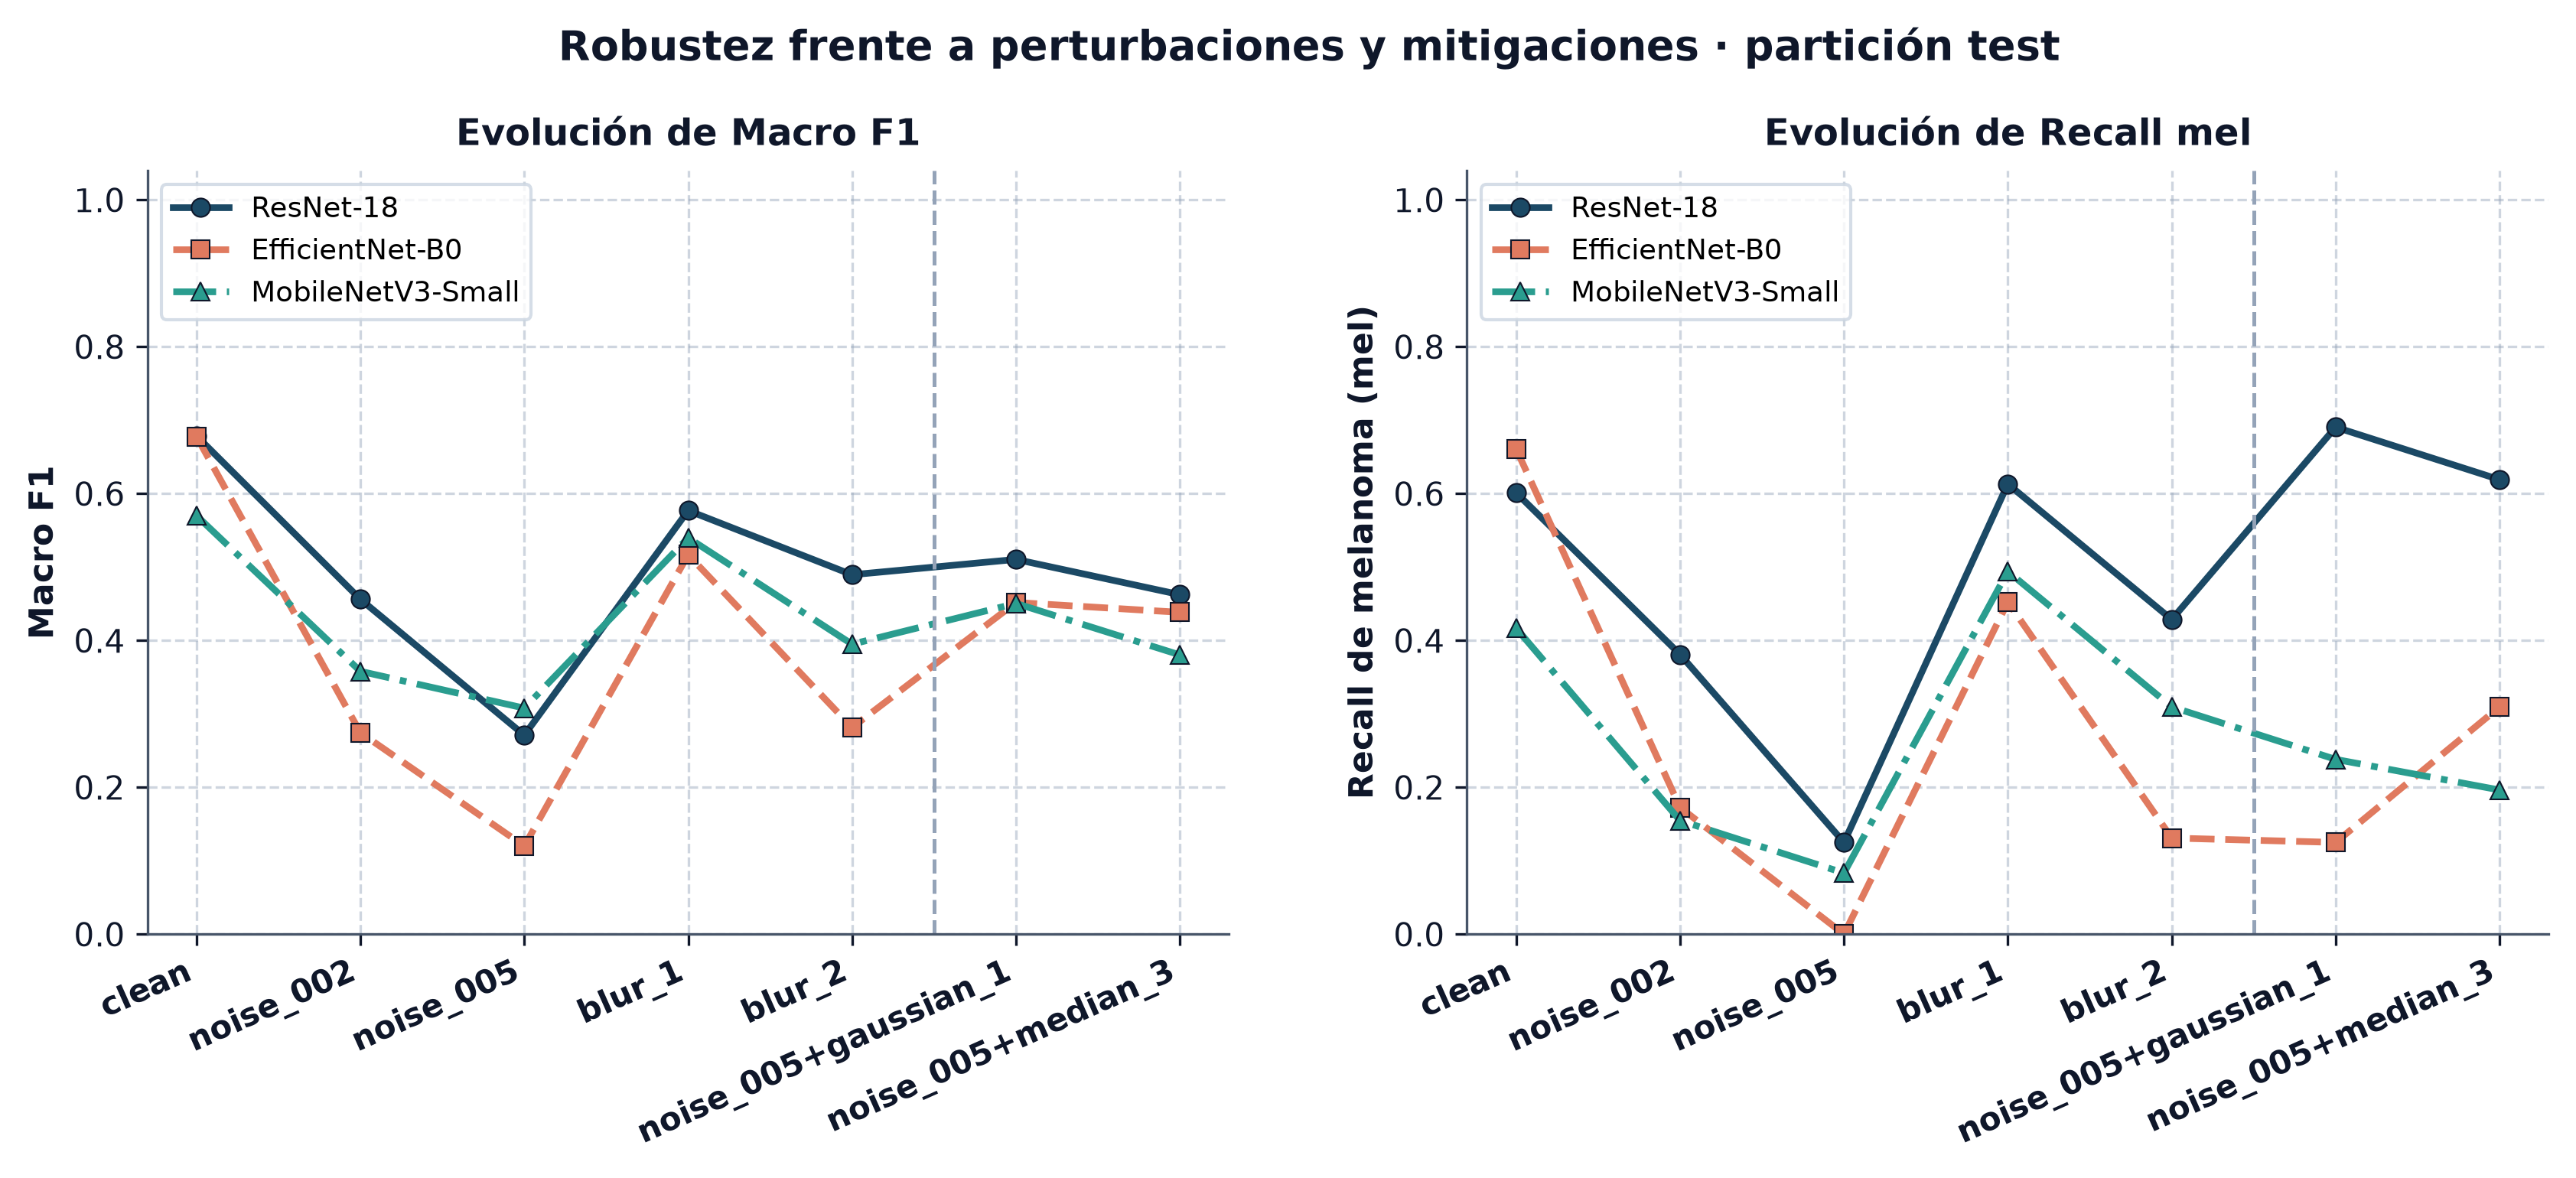
\includegraphics[width=0.96\textwidth]{comparacion_robustez.png}
\caption{Evolución de Macro~F1 (izquierda) y sensibilidad de melanoma (derecha) frente a las cinco condiciones base y las dos variantes de mitigación espacial sobre \texttt{noise\_005}.}
\label{fig:comp_rob}
\end{figure}
\FloatBarrier

La degradación frente a perturbaciones revela contrastes marcados entre arquitecturas:
\begin{itemize}[leftmargin=1.4em,itemsep=3pt]
\item \textbf{Fragilidad severa ante ruido gaussiano:} todas las redes sufren más ante ruido aditivo de alta frecuencia que ante desenfoque moderado. \textbf{EfficientNet-B0} resulta la más vulnerable: cae de 0.6778 a 0.2745 en \texttt{noise\_002} y colapsa hasta 0.1201 en \texttt{noise\_005} ($\Delta F1_{\max}=+0.5577$), anulando por completo la detección de melanoma (\textit{Precision} = 0.0000, \textit{Recall} = 0.0000; $\Delta\mathrm{Rec.\ mel}=+0.6607$; $\mathrm{AUC}_{\mathrm{OVR}}=0.4839$). Como hipótesis interpretativa plausible (pendiente de comprobar mediante ablación), esta caída puede asociarse a una mayor sensibilidad de sus bloques iniciales y módulos de atención de canales SE a texturas de alta frecuencia. MobileNetV3-Small presenta menor caída absoluta ($\Delta F1_{\max}=+0.2621$) y conserva 0.3079 en \texttt{noise\_005}, pero parte de una línea base limpia muy inferior (0.5700), por lo que no constituye una alternativa más capaz.
\item \textbf{Estabilidad relativa ante desenfoque:} \textbf{ResNet-18} mantiene los valores absolutos más altos en \texttt{noise\_002} (0.4561), \texttt{blur\_1} (0.5769) y \texttt{blur\_2} (0.4895), mientras EfficientNet-B0 cae bruscamente ante desenfoque intenso (\texttt{blur\_2}: 0.2815). Como hipótesis interpretativa plausible, las conexiones residuales y filtros iniciales más amplios de ResNet-18 podrían tolerar mejor la atenuación de detalle fino sin perder estabilidad en \textit{logits}.
\item \textbf{Mitigación parcial e intercambio Precision/Recall mediante filtrado espacial (Tablas~\ref{tab:res_mit} y~\ref{tab:res_mel_tradeoff}):} el prefiltrado determinista sin reentrenamiento aporta una ganancia en Macro~F1 sobre \texttt{noise\_005} de \textbf{$+0.14$ a $+0.33$} puntos con \texttt{+gaussian\_1} ($+0.1426$ en MobileNetV3-Small, $+0.2394$ en ResNet-18 y $+0.3317$ en EfficientNet-B0). No obstante, los resultados demuestran que \texttt{+gaussian\_1} constituye una \textbf{mitigación parcial} sujeta a un marcado compromiso operativo: en \textbf{ResNet-18}, \texttt{+gaussian\_1} eleva Macro~F1 de 0.2710 a \textbf{0.5104} (Macro~Prec.\ de 0.4003 a 0.6084), $\mathrm{AUC}_{\mathrm{OVR}}$ de 0.8655 a \textbf{0.9342} y el \textit{Recall} de melanoma de 0.1250 a \textbf{0.6905} (TP sube de 21 a 116), pero a costa de duplicar con creces los falsos positivos respecto a \texttt{clean} (de \textbf{92} a \textbf{202}), reduciendo la \textit{Precision} de melanoma de \textbf{0.5233} a \textbf{0.3648} (F1 \texttt{mel} = 0.4774 vs.\ 0.5596 limpio). De forma análoga, \texttt{+median\_3} eleva el \textit{Recall} de melanoma en ResNet-18 a 0.6190 (TP = 104) con 179 falsos positivos (Precision = 0.3675). En \textbf{EfficientNet-B0}, ambos filtros recuperan el ordenamiento probabilístico global ($\mathrm{AUC}$ sube de 0.4839 a 0.9090 con \texttt{+median\_3} y 0.9187 con \texttt{+gaussian\_1}), pero la cobertura de melanoma sigue deprimida (\textit{Recall} = 0.3095 con \texttt{+median\_3} y 0.1250 con \texttt{+gaussian\_1}). En \textbf{MobileNetV3-Small}, \texttt{+gaussian\_1} alcanza 0.4505 en Macro~F1 y 0.2381 en \textit{Recall} de melanoma (\textit{Precision} = 0.6780). El déficit residual frente a \texttt{clean} obedece al alisado de estructuras dermatoscópicas finas y al desplazamiento de frontera de decisión.
\end{itemize}

\FloatBarrier
\subsection{Síntesis comparativa condicionada al protocolo y hardware}
\begin{tcolorbox}[resBox,title={Recomendación académica condicionada sobre GTX~1650 (\texttt{seed=42}, $n=1\,503$)}]
Bajo la receta compartida (\texttt{configs/base.json}), precisión FP32 y presupuesto de 4~GiB de VRAM en GTX~1650, \textbf{ResNet-18} ofrece el mejor compromiso observado desempeño--latencia en HAM10000: registra Macro~F1 = \textbf{0.6786} (Macro~Prec.\ = 0.6591), \textit{Balanced Accuracy} = \textbf{0.7174}, \textit{Accuracy} = \textbf{0.8031} y $\mathrm{AUC}_{\mathrm{OVR}}$ = \textbf{0.9596}, entrena en menor tiempo (\textbf{127.5~s/época}), infiere con mediana \texttt{forward()} de \textbf{7.22~ms} (P95 = 8.09~ms; rango entre corridas $6.86$--$9.46$~ms) con 434.2~MiB de VRAM, conserva mejores métricas bajo desenfoque y ruido moderado, y alcanza la mayor recuperación tras mitigación parcial (\textbf{0.5104} Macro~F1 con \texttt{+gaussian\_1}, con el compromiso de elevar falsos positivos en melanoma de 92 a 202).\\[4pt]
Sin embargo, la diferencia de 0.00084 en Macro~F1 frente a \textbf{EfficientNet-B0} (0.6778; Macro~Prec.\ = \textbf{0.6741}) \textbf{no demuestra superioridad estadística ni equivalencia} (IC95\% \textit{bootstrap} pareado por $1\,118$ \texttt{group\_id}: $[-0.0429, +0.0464]$). EfficientNet-B0 obtiene la mayor sensibilidad limpia en melanoma (\textbf{0.6607}) y F1 en \texttt{akiec} (0.7143), pero requiere mayor latencia (24.60~ms; rango $22.49$--$34.82$~ms), mayor VRAM (805.7~MiB) y exhibe extrema fragilidad frente a ruido aditivo. \textbf{MobileNetV3-Small} minimiza memoria (211.8~MiB), pero penaliza las categorías minoritarias (Macro~F1 = 0.5700; \texttt{mel} recall = 0.4167; \texttt{akiec} F1 = 0.2667) sin ofrecer ventaja de velocidad en esta GPU (22.40~ms; rango $15.26$--$22.40$~ms). Esta recomendación queda condicionada al protocolo, semilla única y hardware evaluado, y \textbf{no constituye validez ni indicación clínica}.
\end{tcolorbox}
\FloatBarrier

\FloatBarrier\section{Discusión y limitaciones del estudio}

\subsection{Validez interna}
El diseño reduce fuentes conocidas de optimismo metodológico: separación por lesión, agrupamiento de duplicados binarios, comprobación de casi-duplicados entre lesiones distintas, aumento restringido a entrenamiento y selección mediante validación. La configuración común (\texttt{configs/base.json}, \texttt{num\_workers=4} comprobado bit-exacto en sesión piloto puntual, \texttt{seed=42}) controla diferencias ajenas a la arquitectura y el registro completo de versiones y semillas en \texttt{run.json} garantiza trazabilidad tras completar los 3 entrenamientos, las 3 validaciones y las 21 pruebas en \texttt{test}.

Estas protecciones no eliminan todos los sesgos. Una receta compartida puede favorecer más a una arquitectura que a otra y no representa necesariamente su óptimo particular tras una búsqueda extensiva de hiperparámetros. Asimismo, los experimentos se ejecutaron con una sola semilla (\texttt{seed=42}) por restricciones de tiempo de cómputo local en FP32, por lo que no se reporta desviación estándar entre múltiples inicializaciones; adicionalmente, la pequeña diferencia observada en Macro~F1 entre ResNet-18 y EfficientNet-B0 ($0.00084$) presenta un intervalo de confianza amplio en \textit{bootstrap} pareado por grupo ($[-0.0429, +0.0464]$). Además, las implementaciones de operadores pueden variar entre entornos de ejecución.

\subsection{Validez externa y uso clínico}
Un test interno procede de la misma colección general y no demuestra rendimiento en otro centro o cámara. La ausencia de \texttt{patient\_id} impide garantizar independencia estricta entre pacientes distintos y la falta de anotaciones completas de fototipo limita análisis de equidad. El sistema desarrollado es estrictamente académico y no reemplaza dermatoscopia clínica, biopsia ni criterio médico profesional.

\begin{table}[htbp]\centering\small
\caption{Síntesis de amenazas a la validez experimental y medidas de mitigación aplicadas.}
\begin{tabularx}{\textwidth}{@{}>{\bfseries\raggedright\arraybackslash}p{3.0cm}>{\raggedright\arraybackslash}p{5.8cm}>{\raggedright\arraybackslash}X@{}}
\toprule
\textbf{Dimensión} & \textbf{Limitación persistente} & \textbf{Mitigación aplicada en el protocolo} \\ \midrule
Validez interna & Ausencia de \texttt{patient\_id}; dos lesiones de un mismo paciente podrían separarse. & Agrupamiento estricto por \texttt{lesion\_id} + SHA-256 y comprobación de casi-duplicados. \\
Validez externa & Colección austríaca/australiana con sesgo hacia piel clara y pocos dispositivos. & Declaración explícita de alcance académico; prohibición de uso clínico. \\
Validez de constructo & Receta única (\texttt{base.json}, \texttt{seed=42}) frente a ajuste fino exhaustivo por arquitectura y multisenilla. & Presupuesto, partición y semilla idénticos; \texttt{test} congelado tras seleccionar en \texttt{val}. \\
Varianza discreta & Clases escasas en \texttt{test} (\texttt{df}: 17, \texttt{vasc}: 21 muestras) y diferencia no concluyente entre dos modelos. & Reporte de Precision, Recall, F1, AUC, matrices de confusión y \textit{bootstrap} pareado por \texttt{group\_id}. \\
\bottomrule
\end{tabularx}
\end{table}

\subsection{Reproducibilidad y alcance excluido}
El grupo conserva los CSV de partición, configuraciones, historiales, checkpoints, predicciones y gráficos reales generados en \texttt{runs/} y \texttt{resultados/}, citando todas las fuentes primarias. El despliegue interactivo (web o móvil) quedó explícitamente excluido del alcance del proyecto por indicación docente, de modo que no forma parte de los entregables finales; las diapositivas de exposición de diez minutos residen en \texttt{presentacion/}.

\FloatBarrier\section{Conclusiones}
\label{sec:conclusiones}

Tras ejecutar íntegramente el protocolo experimental reproducible sobre HAM10000 (10\,015 imágenes correspondientes a 7\,470 lesiones únicas) bajo una receta común (\texttt{configs/base.json}, precisión FP32, \texttt{batch=8}, \texttt{seed=42}) en GPU NVIDIA GTX~1650 (4~GiB VRAM), completando 3 entrenamientos, 3 validaciones y 21 pruebas deterministas sobre la partición \texttt{test} congelada ($n=1\,503$), se establecen cinco conclusiones científicas principales:

\begin{enumerate}[leftmargin=1.5em,itemsep=4pt]
\item \textbf{Protocolo antifuga, integridad y verificación reproducible:} la auditoría integral descartó archivos faltantes y agrupó correctamente las imágenes por \texttt{lesion\_id} y pares idénticos SHA-256 mediante \texttt{StratifiedGroupKFold} ($K=20$), verificando cero fugas entre \texttt{train} (7\,009), \texttt{val} (1\,503) y \texttt{test} (1\,503) bajo la huella fija \texttt{split\_sha256: 583779fb...}. La revisión de casi-duplicados y el piloto de workers fueron comprobaciones puntuales de sesión, con sus limitaciones declaradas. Las \textbf{22/22} pruebas actuales del pipeline/cuaderno (más 4 de descarga), el test protegido y la inspección local del notebook sin modificar artefactos refuerzan la trazabilidad; no constituyen validación clínica ni acreditan ejecución real en Colab.

\item \textbf{Compromiso observado desempeño--latencia en GTX~1650:} bajo el presupuesto de 4~GiB de VRAM y precisión FP32, \textbf{ResNet-18} ofrece el mejor equilibrio operativo observado entre capacidad discriminativa, costo de entrenamiento y velocidad de inferencia. Alcanza \textbf{Macro~F1 = 0.6786}, Macro~Prec.\ = 0.6591, \textit{Balanced Accuracy} = \textbf{0.7174}, \textit{Accuracy} = \textbf{0.8031} y $\mathrm{AUC}_{\mathrm{OVR}}$ = \textbf{0.9596}, entrenando en \textbf{127.5~s/época} (434.2~MiB de VRAM) e infiriendo en \texttt{batch=1} con una latencia mediana \texttt{forward()} de \textbf{7.22~ms} (P95 = 8.09~ms; rango entre corridas $6.86$--$9.46$~ms), más de $3\times$ más rápida que EfficientNet-B0 y MobileNetV3-Small en esta GPU.

\item \textbf{Ausencia de superioridad estadística ni equivalencia entre ResNet-18 y EfficientNet-B0:} \textbf{EfficientNet-B0} obtiene un desempeño global prácticamente indistinguible en Macro~F1 (\textbf{0.6778}, Macro~Prec.\ = \textbf{0.6741}, \textit{Balanced Accuracy} = 0.7025, $\mathrm{AUC}_{\mathrm{OVR}}$ = 0.9587), con una diferencia puntual de apenas $\Delta = 0.00084$ respecto a ResNet-18. El análisis por \textit{bootstrap} pareado sobre los $1\,118$ grupos independientes (\texttt{group\_id}) de \texttt{test} arroja un intervalo de confianza al 95\% de \textbf{$[-0.0429, +0.0464]$}, lo que impide afirmar superioridad estadística o equivalencia entre ambas arquitecturas bajo una única semilla.

\item \textbf{Sensibilidad limpia en melanoma frente a compacidad paramétrica:} \textbf{EfficientNet-B0} registra la mayor sensibilidad limpia en melanoma (\textbf{0.6607}; 111/168 aciertos, $\mathrm{AUC}_{\mathrm{OVR}}=0.9113$ en \texttt{mel}) y el mejor F1 en \texttt{akiec} (0.7143), a costa de duplicar prácticamente el uso de VRAM (805.7~MiB), el tiempo por época (188.6~s) y triplicar la latencia de inferencia (24.60~ms; rango $22.49$--$34.82$~ms). Por su parte, \textbf{MobileNetV3-Small} minimiza parámetros (1\,525\,031) y VRAM (\textbf{211.8~MiB}), pero sufre una severa pérdida de cobertura en categorías minoritarias y críticas (Macro~F1 = \textbf{0.5700}, \textit{Balanced Accuracy} = 0.5604, \texttt{mel} recall = 0.4167 con 70/168 aciertos, \texttt{akiec} F1 = 0.2667 y \texttt{df} F1 = 0.3846) sin ventaja de latencia GPU en \texttt{batch=1} (22.40~ms; rango $15.26$--$22.40$~ms), confirmando que menos parámetros no garantizan menor latencia ni desempeño balanceado.

\item \textbf{Vulnerabilidad ante ruido gaussiano y mitigación parcial con intercambio Precision/FP:} todas las redes muestran mayor fragilidad ante ruido aditivo de alta frecuencia que frente a desenfoque moderado; en \texttt{noise\_005}, EfficientNet-B0 colapsa a \textbf{0.1201} de Macro~F1 y \textbf{0.0000} de sensibilidad en melanoma ($\mathrm{AUC}_{\mathrm{OVR}}=0.4839$), mientras ResNet-18 preserva los mayores valores relativos en \texttt{noise\_002} (0.4561), \texttt{blur\_1} (0.5769) y \texttt{blur\_2} (0.4895). El prefiltrado determinista con \texttt{+gaussian\_1} sobre \texttt{noise\_005} aporta ganancias de $+0.14$ a $+0.33$ puntos en Macro~F1 sin reentrenamiento (elevando a ResNet-18 de 0.2710 a \textbf{0.5104} en Macro~F1, \textbf{0.9342} en $\mathrm{AUC}_{\mathrm{OVR}}$ y \textbf{0.6905} en \texttt{mel} recall), pero constituye una mitigación parcial que desplaza el umbral operativo y más que duplica los falsos positivos de melanoma en ResNet-18 (de \textbf{92} en \texttt{clean} a \textbf{202} en \texttt{+gaussian\_1}, reduciendo la \textit{Precision} de \texttt{mel} de \textbf{0.5233} a \textbf{0.3648}).
\end{enumerate}

\FloatBarrier\clearpage\section{Recomendaciones y trabajo futuro}
\label{sec:recomendaciones}

A partir de los resultados verificados y de las limitaciones metodológicas identificadas en la discusión, se formulan recomendaciones operativas para la selección de modelos, el manejo del pipeline experimental y las líneas de continuación científica del proyecto.

\subsection{Recomendaciones de selección de arquitectura por escenario}
\begin{itemize}[leftmargin=1.4em,itemsep=4pt]
\item \textbf{Escenario predeterminado de equilibrio y baja latencia (elegir ResNet-18):} se recomienda \textbf{ResNet-18} cuando el despliegue experimental opere en GPU de gama media o recursos restringidos (4~GiB VRAM, FP32), se requiera baja latencia por imagen en \texttt{batch=1} (mediana de \textbf{7.22~ms}), tiempos cortos de entrenamiento (\textbf{127.5~s/época}) o mayor resiliencia relativa frente a desenfoque (\texttt{blur\_1}, \texttt{blur\_2}), ruido moderado (\texttt{noise\_002}) y recuperación parcial tras prefiltrado espacial (\texttt{+gaussian\_1}).
\item \textbf{Escenario de datos limpios con prioridad en sensibilidad de melanoma (considerar EfficientNet-B0):} puede considerarse \textbf{EfficientNet-B0} únicamente cuando las capturas dermatoscópicas estén limpias y libres de ruido aditivo de alta frecuencia, exista holgura de memoria (805.7~MiB de VRAM) y de latencia (24.60~ms en \texttt{batch=1}), y el criterio prioritario sea maximizar la sensibilidad limpia de melanoma (\textbf{0.6607}) o el desempeño en \texttt{akiec} (Precision = 0.8571, F1 = 0.7143). Su uso no es recomendable en presencia de ruido sin reentrenamiento específico.
\item \textbf{Escenario de restricción extrema de memoria frente a cobertura minoritaria (evitar MobileNetV3-Small):} debe evitarse \textbf{MobileNetV3-Small} siempre que importe la detección de categorías minoritarias o de alto riesgo (\texttt{mel} recall = 0.4167, \texttt{akiec} recall = 0.1633, \texttt{df} recall = 0.2941) o cuando se busque acelerar la inferencia GPU en \texttt{batch=1} (22.40~ms frente a 7.22~ms en ResNet-18). Su ventaja se restringe exclusivamente al menor consumo de VRAM (211.8~MiB) y tamaño de parámetros (1.53~M).
\end{itemize}

\subsection{Recomendaciones sobre preprocesamiento, filtrado y evaluación}
\begin{itemize}[leftmargin=1.4em,itemsep=4pt]
\item \textbf{Advertencia operativa sobre \texttt{+gaussian\_1} y el compromiso Recall/Precision/FP:} el prefiltrado determinista mediante \texttt{+gaussian\_1} (o \texttt{+median\_3}) sobre imágenes afectadas por \texttt{noise\_005} no debe interpretarse como una recuperación equivalente al dato limpio. Aunque en ResNet-18 eleva el \textit{Recall} de melanoma a \textbf{0.6905} (116/168), simultáneamente reduce la \textit{Precision} de melanoma de \textbf{0.5233} a \textbf{0.3648} y eleva los falsos positivos de \textbf{92} (\texttt{clean}) a \textbf{202}; además, en EfficientNet-B0 la cobertura de \texttt{mel} permanece deprimida (0.1250 con \texttt{+gaussian\_1}). Cualquier aplicación de filtrado en inferencia debe acompañarse del reporte conjunto de \textit{Precision}, \textit{Recall} y conteo TP/FP/FN.
\item \textbf{Preservación estricta de \texttt{split.csv} y control antifuga:} en extensiones o reentrenamientos futuros sobre HAM10000, debe conservarse inalterado el manifiesto fijo \texttt{data/processed/split.csv} (\texttt{split\_sha256: 583779fb...}), manteniendo la agrupación por \texttt{lesion\_id} y duplicados binarios, el cálculo exclusivo de estadísticas ($\mu$, $\sigma$) y pesos de clase $w_c$ sobre \texttt{train}, y la restricción de aumento de datos únicamente a entrenamiento, resguardando la partición \texttt{test} tras la confirmación explícita \texttt{-{}-confirmar-test}.
\item \textbf{Medición empírica de latencia en el hardware objetivo:} no debe inferirse la velocidad real de inferencia a partir del conteo de parámetros o FLOPs teóricos. Es indispensable medir la latencia mediana y P95 de \texttt{forward()} en el mismo hardware, precisión y tamaño de lote objetivo (\texttt{batch=1}), aplicando calentamiento previo y sincronización explícita de CUDA, y reportando el rango de dispersión entre corridas.
\end{itemize}

\subsection{Líneas de trabajo futuro}
\begin{enumerate}[leftmargin=1.5em,itemsep=4pt]
\item \textbf{Evaluación con múltiples semillas y ajuste por arquitectura:} repetir los entrenamientos y pruebas con múltiples semillas independientes (p.\ ej., 3--5 semillas) y explorar recetas de regularización diferenciadas por familia arquitectónica para cuantificar la varianza inter-semilla y estrechar la incertidumbre estadística observada entre ResNet-18 y EfficientNet-B0.
\item \textbf{Entrenamiento robusto mediante aumento con ruido y desenfoque:} incorporar perturbaciones gaussianas y desenfoque controlado dentro de la política de aumento en \texttt{train} para evaluar si las redes adquieren invarianza frente a degradaciones de alta frecuencia sin inducir el incremento severo de falsos positivos observado con \texttt{+gaussian\_1} post-hoc.
\item \textbf{Calibración probabilística y optimización de umbrales clínicos:} estudiar métodos de calibración (como escalado de temperatura en \texttt{val}) y ajuste de umbrales de decisión específicos para \texttt{mel}, analizando curvas de costo clínico entre falsos negativos críticos y sobrecarga por falsos positivos.
\item \textbf{Validación externa multicéntrica y auditoría de equidad:} evaluar los modelos entrenados sobre cohortes dermatoscópicas externas de distintos centros y dispositivos, incorporando identificadores de paciente (\texttt{patient\_id}) y metadatos de fototipo cutáneo para verificar la generalización real fuera del dominio HAM10000.
\end{enumerate}


\FloatBarrier
\clearpage
\renewcommand{\refname}{Referencias bibliográficas}
\phantomsection
\addcontentsline{toc}{section}{Referencias bibliográficas}
\bibliographystyle{IEEEtran}
\bibliography{referencias}

\clearpage
\appendix
\addtocontents{toc}{\protect\addvspace{6pt}\protect\renewcommand{\protect\cftsecpresnum}{Apéndice~}\protect\setlength{\protect\cftsecnumwidth}{6.4em}}
\FloatBarrier\section{Guía operativa de reproducción y contratos de código}

\subsection{Comandos locales principales}
Desde el directorio \texttt{proyecto\_ham10000}, utilizando el entorno GPU aislado \texttt{..\textbackslash.venv}:

\begin{lstlisting}[language=bash,caption={Validación, exportación de carpetas y entrenamiento base.}]
..\.venv\Scripts\python.exe python\ejecutar.py validar --datos ..\descargaDataSet\HAM10000 --split data\processed\split.csv
..\.venv\Scripts\python.exe python\ejecutar.py exportar --datos ..\descargaDataSet\HAM10000 --split data\processed\split.csv --salida data\processed
..\.venv\Scripts\python.exe python\ejecutar.py entrenar --modelo resnet18 --datos ..\descargaDataSet\HAM10000 --split data\processed\split.csv --config configs\base.json --salida runs
\end{lstlisting}

Repetir el comando de entrenamiento con \texttt{efficientnet\_b0} y \texttt{mobilenet\_v3\_small}, añadiendo \texttt{-{}-resume} en caso de reanudación tras una interrupción.

\subsection{Evaluación protegida y consolidación}
\begin{lstlisting}[language=bash,caption={Evaluación en test congelado, mitigación espacial, comparación y compilación.}]
..\.venv\Scripts\python.exe python\ejecutar.py evaluar --checkpoint runs\resnet18_seed42\best.pt --datos ..\descargaDataSet\HAM10000 --split data\processed\split.csv --salida runs\resnet18_seed42\evaluacion --particion test --confirmar-test --condicion clean
..\.venv\Scripts\python.exe python\ejecutar.py evaluar --checkpoint runs\resnet18_seed42\best.pt --datos ..\descargaDataSet\HAM10000 --split data\processed\split.csv --salida runs\resnet18_seed42\evaluacion --particion test --confirmar-test --condicion noise_005 --mitigacion median_3
..\.venv\Scripts\python.exe python\ejecutar.py comparar --runs runs --salida resultados
..\.venv\Scripts\python.exe latex\compilar.py
\end{lstlisting}

Las cinco condiciones base usan \texttt{-{}-mitigacion none} (guardando en \texttt{\{split\}\_\allowbreak\{condicion\}}), mientras que \texttt{median\_3} y \texttt{gaussian\_1} guardan en \texttt{\{split\}\_\allowbreak\{condicion\}\_\allowbreak\{mitigacion\}} sin sobrescribir las corridas base. Al ejecutar \texttt{comparar}, se consolidan \texttt{comparacion.csv}, \texttt{curvas\_*.png}, \texttt{confusion\_*.png}, curvas ROC OVR (\texttt{roc\_*.png}, \texttt{roc\_\allowbreak comparativa\_*.png}), \texttt{comparacion\_\allowbreak metricas.png} y \texttt{comparacion\_\allowbreak robustez.png}.

Para evaluar en CPU un checkpoint CUDA sin editarlo se añaden \texttt{-{}-device cpu -{}-num-workers 0} y una salida independiente. La consolidación admite \texttt{-{}-subcarpeta-evaluacion evaluacion} para no mezclar mediciones alternativas; rechaza duplicados y entornos de inferencia incompatibles. El notebook deja entrenamiento, evaluación, figuras y exportación desactivados por defecto, y escribe salidas nuevas en \texttt{resultados\_notebook/}. No sustituye automáticamente cifras ni figuras del informe.

\subsection{Arquitectura modular del paquete \texttt{python/ham10000}}
Para evitar divergencias entre ejecución local y nube, toda la lógica de datos, modelos, entrenamiento, métricas y gráficos reside en un único paquete modular invocado desde \texttt{ejecutar.py} (Tabla~\ref{tab:modulos}).

\begin{table}[htbp]\centering\small
\caption{Organización modular y responsabilidad de cada archivo en \texttt{python/}.}
\label{tab:modulos}
\begin{tabularx}{\textwidth}{@{}>{\ttfamily}p{4.3cm}>{\raggedright\arraybackslash}X@{}}
\toprule
\textbf{\textrm{Módulo}} & \textbf{Responsabilidad técnica verificada} \\ \midrule
ejecutar.py & Interfaz CLI unificada (\texttt{preparar}, \texttt{validar}, \texttt{exportar}, \texttt{entrenar}, \texttt{evaluar}, \texttt{figuras}, \texttt{comparar}). \\
ham10000/\_\_init\_\_.py & Define constantes canónicas de 7 clases (\texttt{CLASES}) y 3 arquitecturas (\texttt{MODELOS}). \\
ham10000/io.py & Lectura UTF-8 BOM-safe, escritura atómica de CSV/JSON y cálculo de \texttt{sha256}. \\
ham10000/prepare.py & Auditoría, agrupación \textit{Union-Find}, \texttt{StratifiedGroupKFold(20)}, exportación y verificación de fugas. \\
ham10000/data.py & \textit{Letterbox} $224\times224$, aumento determinista en \texttt{train}, normalización ImageNet, perturbaciones y mitigación espacial. \\
ham10000/models.py & Carga de pesos \texttt{IMAGENET1K\_V1}, reemplazo de cabeza a 7 clases y congelado seguro de \textit{BatchNorm}. \\
ham10000/metrics.py & Macro Precision/F1, Balanced Accuracy, \texttt{Recall mel}, $\mathrm{AUC}_{\mathrm{OVR}}$, reporte por clase y matriz $7\times7$. \\
ham10000/engine.py & Entrenamiento en 2 fases, checkpoints/reanudación protegidos, test confirmado, mitigación y evaluación CUDA/CPU sin editar el checkpoint. \\
ham10000/artifacts.py & Verifica procedencia, muestras y probabilidades antes de reutilizar evaluaciones; detecta archivos incompletos. \\
ham10000/plots.py & Generación de las 11 figuras descriptivas, consolidación (\texttt{comparacion.csv}), curvas ROC y gráficos comparativos. \\
../colab/runtime.py & Inicialización local/Colab y extracción segura, integradas en el notebook desde su generador. \\
\bottomrule
\end{tabularx}
\end{table}

\FloatBarrier
\subsection{Contratos esenciales de implementación}
Los módulos centrales desacoplan la ingestión de datos, la construcción de arquitecturas y el cálculo de métricas para compartir exactamente la misma lógica entre Windows y Google Colab:

\begin{lstlisting}[language=Python,caption={Adaptación homogénea de las tres arquitecturas y congelamiento seguro de BatchNorm (\texttt{models.py}).}]
def construir(name, pretrained=True):
    weights = {
        "resnet18": models.ResNet18_Weights.IMAGENET1K_V1,
        "efficientnet_b0": models.EfficientNet_B0_Weights.IMAGENET1K_V1,
        "mobilenet_v3_small": models.MobileNet_V3_Small_Weights.IMAGENET1K_V1,
    }
    model = getattr(models, name)(weights=weights[name] if pretrained else None)
    if name == "resnet18":
        model.fc = nn.Linear(model.fc.in_features, len(CLASES))
    else:
        model.classifier[-1] = nn.Linear(model.classifier[-1].in_features, len(CLASES))
    return model, str(weights[name]) if pretrained else "sin_preentrenamiento"
\end{lstlisting}

\begin{lstlisting}[language=Python,caption={Adaptación geométrica isotrópica y perturbación determinista por imagen (\texttt{data.py}).}]
def letterbox(image, size=224):
    image = ImageOps.exif_transpose(image).convert("RGB")
    image = ImageOps.contain(image, (size, size), method=Image.Resampling.BILINEAR)
    canvas = Image.new("RGB", (size, size), tuple(round(x * 255) for x in MEAN))
    canvas.paste(image, ((size - image.width) // 2, (size - image.height) // 2))
    return canvas
\end{lstlisting}

\subsection{Secuencia sugerida para la exposición de diez minutos}
\begin{enumerate}[leftmargin=1.6em,itemsep=3pt]
\item \textbf{Minuto 0--1:} planteamiento de clasificación dermatoscópica en HAM10000 y alcance académico.
\item \textbf{Minuto 1--3:} desbalance 58.3:1, auditoría SHA-256 y partición fija agrupada por \texttt{lesion\_id}.
\item \textbf{Minuto 3--5:} diferencias estructurales entre ResNet-18, EfficientNet-B0 y MobileNetV3-Small.
\item \textbf{Minuto 5--8:} resultados comparativos reales, matrices de confusión, sensibilidad de melanoma, robustez y eficiencia.
\item \textbf{Minuto 8--10:} limitaciones, conclusiones y preguntas.
\end{enumerate}

\clearpage
\FloatBarrier\section{Trazabilidad, criterios de aceptación y glosario}

\subsection{Correspondencia entre requerimientos y artefactos}
{\small\setlength{\tabcolsep}{6pt}\renewcommand{\arraystretch}{1.1}
\begin{longtable}{@{}>{\bfseries\raggedright\arraybackslash}p{4.2cm}>{\raggedright\arraybackslash}p{8.0cm}>{\raggedright\arraybackslash}p{3.4cm}@{}}
\caption{Matriz de trazabilidad entre requisitos docentes y artefactos del proyecto.}\\
\toprule
\textbf{Requerimiento} & \textbf{Artefacto verificable} & \textbf{Estado} \\ \midrule\endfirsthead
\toprule
\textbf{Requerimiento} & \textbf{Artefacto verificable} & \textbf{Estado} \\ \midrule\endhead
Tres arquitecturas CNN & Módulo \texttt{models.py} y \texttt{configs/base.json} (\texttt{num\_workers=4}) & Completado \\
Ingesta y auditoría & \texttt{auditoria.json}, SHA-256 y barrido $\mathrm{RMSE}$ (comprobación puntual de sesión; limitación perceptual vigente) & Ejecutado \\
Partición sin fuga & \texttt{split.csv} (\texttt{583779fb...}) y carpetas \texttt{train/val/test} & Ejecutado \\
Preprocesamiento & \texttt{data.py}, \texttt{estadisticas.json} y mosaicos & Ejecutado \\
Piloto y pruebas unitarias & Comprobación puntual de sesión (\texttt{num\_workers=0/4}) sin reporte independiente; 22/22 pruebas del pipeline/cuaderno + 4 de descarga & Ejecutado \\
Entrenamiento comparativo & 3 corridas completas (\texttt{best.pt}/\texttt{last.pt}, \texttt{history.csv}, \texttt{curvas\_*.png}) & Completado \\
Evaluación multimétrica & 3 \texttt{val} + 3 \texttt{test\_clean}, \texttt{comparacion.csv}, matrices, curvas ROC (\texttt{roc\_*.png}, \texttt{roc\_comparativa\_test\_clean.png}) y \texttt{comparacion\_metricas.png} & Ejecutado \\
Robustez al ruido & 18 corridas perturbadas en \texttt{test} (4 perturbaciones base + \texttt{median\_3}/\texttt{gaussian\_1} por modelo) y \texttt{comparacion\_robustez.png} & Ejecutado \\
Eficiencia GPU & Latencia \texttt{forward()} \texttt{batch=1} (mediana/P95), VRAM pico y s/época en GTX~1650 & Ejecutado \\
Artículo científico IEEE & \texttt{latex/paper\_ieee.pdf} (8 págs.\ \texttt{IEEEtran}) & Completado \\
Informe ampliado & \texttt{latex/main.pdf} (resultados reales, Precision por clase y discusión integrados) & Completado \\
Exposición 10 min & Diapositivas en carpeta \texttt{presentacion/} & Completado \\
Cuaderno integrado & Mismo título, paquete y split; ejecución local de inspección, rama Colab simulada; nube real no acreditada & Verificado localmente \\
Despliegue funcional & Excluido del alcance por indicación docente & Excluido (no requerido) \\
\bottomrule
\end{longtable}
}

\subsection{Listas de comprobación y glosario}
{\small\setlength{\parskip}{3pt}
Lista de comprobación verificada: intérprete \texttt{.venv}, GPU GTX~1650 (driver 621.01, PyTorch \texttt{2.11.0+cu128}), piloto puntual de equivalencia bit-exacta de workers 4 frente a 0 (sin reporte independiente), manifiesto fijo y esquema/sintaxis del notebook. La revisión del cuaderno ejecutó sus 11 celdas de código localmente, verificó los hashes de 10\,015 originales y conservó sin cambios 61 artefactos experimentales; probó además la rama Colab mediante simulación, no una cuenta externa. Antes del test experimental se congelaron los tres checkpoints seleccionados en \texttt{val} y las cinco condiciones más mitigaciones (21 evaluaciones test). No se relanzaron entrenamientos HAM10000 al revisar el notebook.

\begin{description}[leftmargin=1.4em,itemsep=1pt,topsep=3pt]
\item[Split:] asignación de muestras a \texttt{train}, \texttt{val} y \texttt{test} agrupada por \texttt{lesion\_id} y SHA-256.
\item[Macro F1:] promedio no ponderado de $F1_c$ sobre las siete clases diagnósticas.
\item[Leakage:] filtración de información correlacionada entre entrenamiento y evaluación.
\item[Transfer learning:] adaptación de pesos preentrenados ImageNet mediante congelamiento inicial de extractor y ajuste fino diferencial.
\item[VRAM:] memoria gráfica dedicada de la GPU (4~GiB en GTX 1650), distinta de la RAM del sistema.
\end{description}

\subsection{Responsabilidad académica del Grupo N.\ 9}
Los integrantes consignados (Choquenaira Quispe, Noe Franklin -- 133962; Porroa Sivana, Yeni Ruth -- 120893; Colque Galindo, Jean Franco -- 193109) asumen la revisión conjunta de método, código, tablas comparativas, resultados experimentales reales y conclusiones tras completar íntegramente el protocolo experimental.
}


\end{document}
